% Arquivo LaTeX de exemplo de dissertação a ser apresentados ao PPGI do Centro de Ciências Exatas e Tecnologia (CCET) - UNIRIO
%
% Versão 1.0: Sábado, 14 de Setembro de 2013
%
% Criação: Wander dos Santos Vasconcellos
\documentclass[12pt, oneside, a4paper, final]{report}
\usepackage[a4paper,left=3.0cm,right=3.0cm,top=2.5cm,bottom=2.5cm]{geometry} % definição das margens
\usepackage{setspace} % habilitando o espaço entre linhas
\usepackage{titlesec}
\usepackage{dirtytalk}
\usepackage{csquotes}
\usepackage[normalem]{ulem} % habilitando palavras sublinhadas
\usepackage{amsthm, amssymb, amsmath, pxfonts} % permite símbolos matemáticos
\usepackage{mathrsfs} % permite uso de fontes para conjuntos
\usepackage{graphicx} % permite inserção de figuras
%\usepackage{algorithmic}	% pacote para uso na definição do ambiente para algoritmos
\usepackage{framed}
\usepackage{booktabs}
\usepackage{comment}
\usepackage{hyperref}
\usepackage{xr}
\usepackage{makeidx}
\usepackage{adjustbox}

\usepackage[mathcal]{euler}
\usepackage{fontspec}
\usepackage{polyglossia} 
\setdefaultlanguage{english}
\defaultfontfeatures{Ligatures=TeX}
\setmainfont[Extension=.ttf,
             BoldFont=timesbd,
             ItalicFont=timesi,
             BoldItalicFont=timesbi]{times} % habilitando a fonte do texto
\setromanfont[Extension=.ttf,
             BoldFont=timesbd,
             ItalicFont=timesi,
             BoldItalicFont=timesbi]{times}
\setsansfont[Extension=.ttf,
             BoldFont=arialbd,
             ItalicFont=ariali,
             BoldItalicFont=arialbi]{arial}
\setmonofont[Extension=.ttf,
             BoldFont=courbd,
             ItalicFont=couri,
             BoldItalicFont=courbi]{cour}


%\linespread{1.5} % espaço entre linhas de 1.5
\doublespacing
\setlength{\parskip}{10pt} % espaço entre parágrafos
\setcounter{secnumdepth}{3} % habilita a variável \thesubsubsection
\setcounter{tocdepth}{3} % Índice até subsubsection
\titleformat{\chapter}[hang]{\fontsize{16}{16}\normalfont\bfseries\filleft\selectfont}{\thechapter.}{0pt}{\normalfont\bfseries}
\titlespacing{\chapter}{0pt}{72pt}{60pt}
\titleformat{\section}[hang]{\fontsize{12}{12}\normalfont\bfseries\selectfont}{\thesection}{0pt}{\normalfont\bfseries}
\titlespacing{\section}{0pt}{24pt}{12pt}
\titleformat{\subsection}[hang]{\fontsize{12}{12}\normalfont\bfseries\selectfont}{\thesubsection}{0pt}{\normalfont\bfseries}
\titlespacing{\subsection}{0pt}{12pt}{6pt}
\titleformat{\subsubsection}[hang]{\fontsize{12}{12}\normalfont\bfseries\selectfont}{\thesubsubsection}{0pt}{\normalfont\bfseries}
\titlespacing{\subsubsection}{0pt}{6pt}{3pt}


\hypersetup{
		pdftitle={\@title}, 
		pdfauthor={\@author},
		colorlinks=true,       		% false: boxed links; true: colored links
    	linkcolor=black,          	% color of internal links
    	citecolor=black,        		% color of links to bibliography
    	filecolor=black,      		% color of file links
		urlcolor=black}

\graphicspath{ {imgs/} }		% Local onde as imagens serão procuradas

\usepackage[titletoc]{appendix}

\usepackage{lastpage}
\usepackage{float}

\usepackage{listings}
\lstset{language=SQL,morekeywords={PREFIX,java,rdf,rdfs,url}}


\usepackage[usenames,dvipsnames,svgnames,table]{xcolor}				% Controle das cores
\definecolor{orange}{rgb}{1,0.5,0}

\usepackage{enumerate}
\renewcommand{\labelitemi}{$-$}

%INICIO CONFIGURAÇÃO DO PACOTE DE ALGORITMO
\usepackage[chapter]{algorithm}
\usepackage{algorithmicx}
\usepackage{algpseudocode}
\usepackage{amsmath}

\makeatletter
\renewcommand{\ALG@name}{Algorithm}
\renewcommand{\listalgorithmname}{List of \ALG@name s}
\algrenewcommand\ALG@beginalgorithmic{\footnotesize}
\makeatother

\renewcommand{\algorithmicend}{\textbf{end}}
\renewcommand{\algorithmicif}{\textbf{if}}
\renewcommand{\algorithmicthen}{\textbf{then}}
\renewcommand{\algorithmicdo}{\textbf{do}}
\renewcommand{\algorithmicwhile}{\textbf{while}}
\renewcommand{\algorithmicfor}{\textbf{for}}
\renewcommand{\algorithmicrepeat}{\textbf{repeat}}
\renewcommand{\algorithmicreturn}{\textbf{return}}
\renewcommand{\algorithmicelse}{\textbf{else}}
\renewcommand{\algorithmicuntil}{\textbf{until}}
\renewcommand{\algorithmicforall}{\textbf{for each}}
%FIM CONFIGURAÇÃO DO PACOTE DE ALGORITMO

\newtheorem{theorem}{Teorema}

\usepackage{longtable} %tabelas com mais de uma pagina
\usepackage{ltcaption}
\renewcommand\CaptionLabelFont{\normalsize}
\renewcommand\CaptionTextFont{\normalsize}
\setlength{\LTcapwidth}{\linewidth}

\usepackage{lscape} %pacote para landscape

\usepackage{colortbl} %cor para as tabelas
\definecolor{tblH}{rgb}{1,1,1}
\definecolor{tblO}{rgb}{0.9,0.9,0.9}
\definecolor{tblE}{rgb}{0.6,0.6,0.6}
\usepackage{hhline} %cor para as tabelas
\usepackage{pdfpages}

\usepackage{graphicx}
\usepackage{subcaption}
\usepackage{glossaries}
\usepackage{rotating}
\usepackage{ltxtable}
\makeglossaries


\hyphenation{wiki-pe-dia} %¬¬¬¬¬¬¬¬¬¬¬¬¬¬¬¬¬¬0o9xdssssssss like en-cy-clo-pe-dia

\begin{document}
 	
    \pagestyle{empty}
    % Início da capa
\begin{figure}[!h]
    \centering
    
\includegraphics[scale=.25]{unirio}
\end{figure}
\begin{center}
    UNIVERSIDADE FEDERAL DO ESTADO DO RIO DE JANEIRO \\ CENTRO DE CIÊNCIAS EXATAS E TECNOLOGIA \\ PROGRAMA DE PÓS-GRADUAÇÃO EM INFORMÁTICA
    \vskip 7.0cm

   TagTheWeb: USING WIKIPEDIA CATEGORIES TO AUTOMATICALLY CATEGORIZE TEXTUAL-BASED RESOURCES ON THE WEB
    \vskip 1.0cm

    Jerry Fernandes Medeiros
    \vskip 2.0cm
\end{center}
\begin{flushright}
    \textbf{Orientadores}

    Bernardo Pereira Nunes

    Sean Wolfgand Matsui Siqueira
\end{flushright}
\vspace{\stretch{1}} % Posiciona o próximo texto no fim da página.
\begin{center}
    RIO DE JANEIRO, RJ - BRASIL \\ SETEMBRO DE 2018
\end{center}
% Fim da capa
    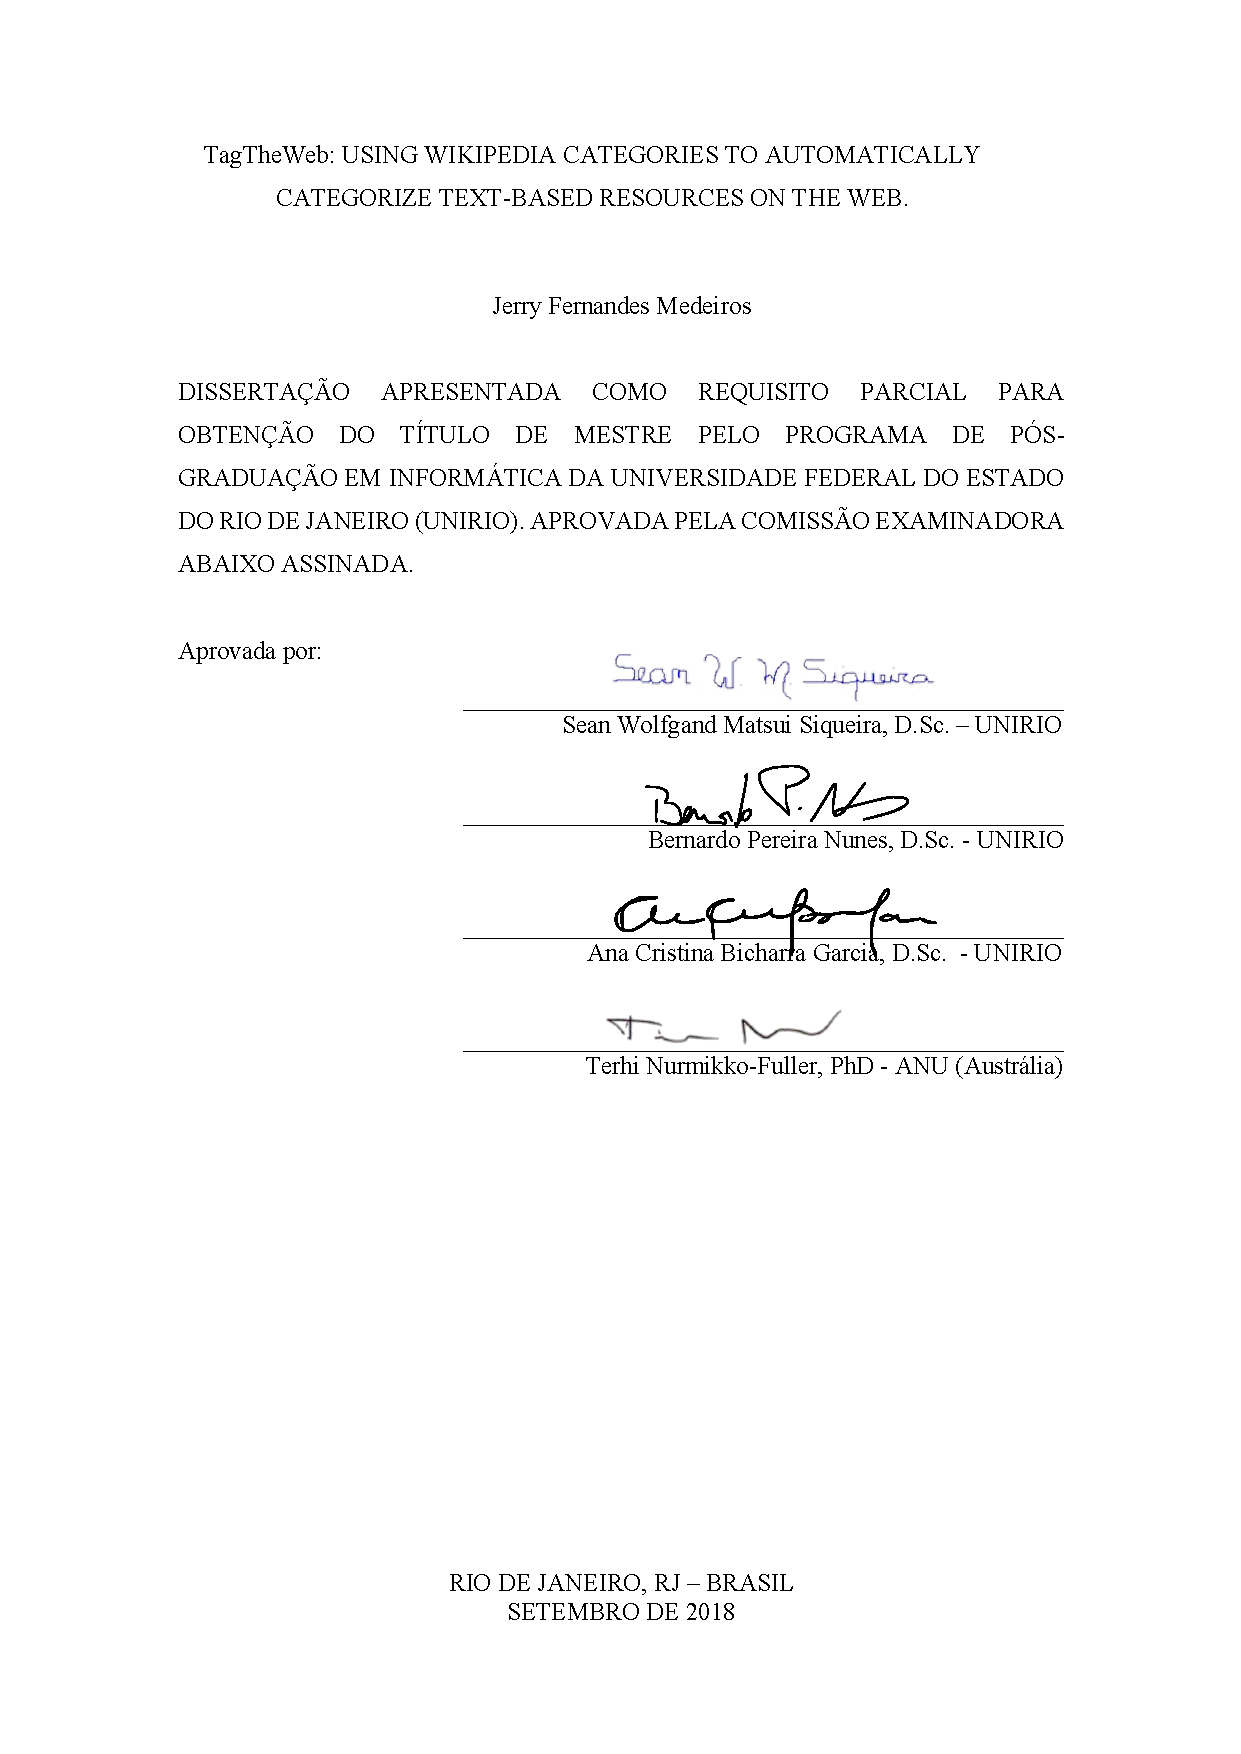
\includepdf[pages={1}]{folha_rosto_final.pdf}
    \nopagecolor
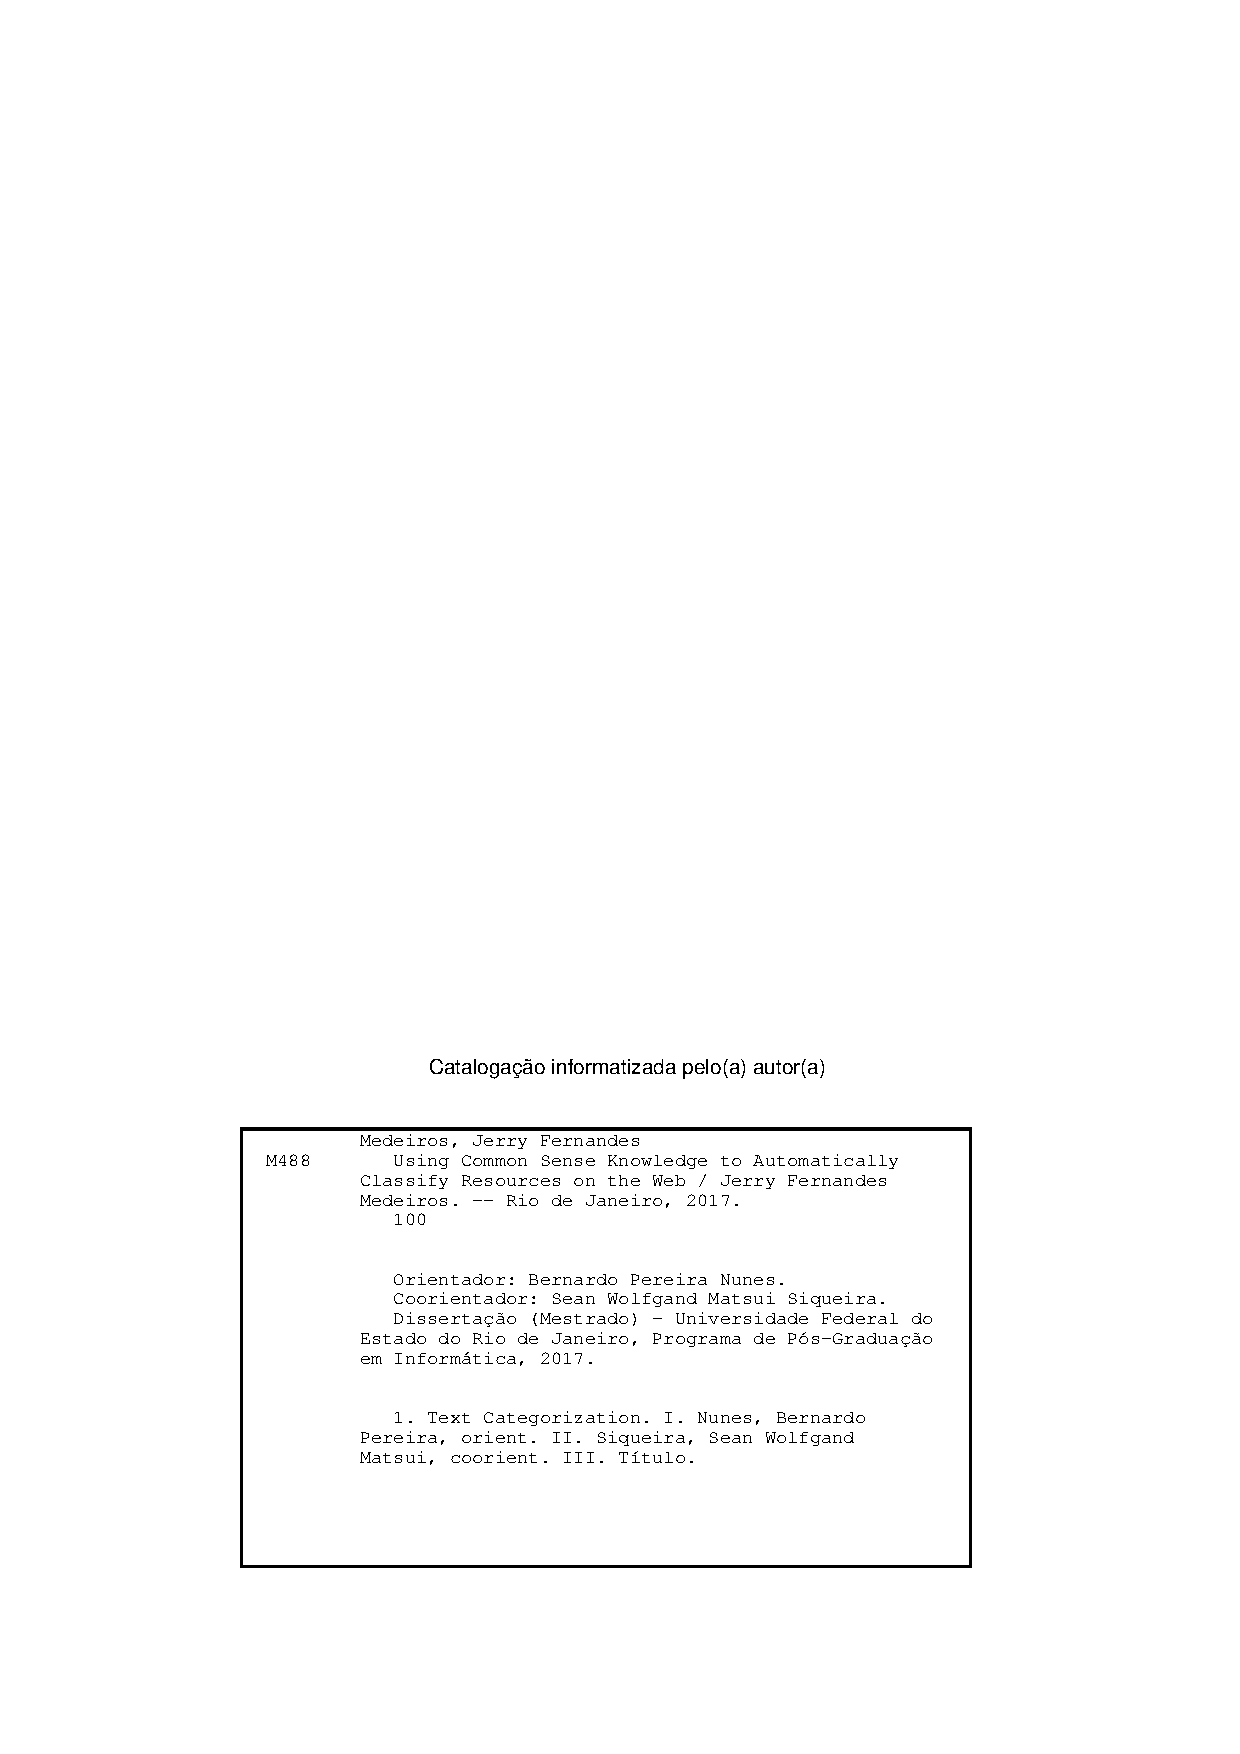
\includepdf[pages={1}]{ficha_catalografica.pdf}
    \pagestyle{plain}
    \pagenumbering{roman}
    \begingroup
    \singlespacing
        % Início da Dedicatória
\vspace*{\stretch{1}} % Posiciona o próximo texto no fim da página.
\hspace{8cm}{ %margem 
\begin{minipage}{6cm} %mantem a margem nas proximas linhas



\end{minipage}
}

% Fim da dedicatória
       % % Início do Agradecimento
\begin{flushright}
    \vspace*{72pt}
    \fontsize{16}{16}\selectfont \textbf{Acknowledgement}
    \vspace{60pt}
\end{flushright}

% Fim do agradecimento
    \endgroup
    % Início do abstract
Medeiros, Jerry Fernandes. \textbf{TagTheWeb: USING WIKIPEDIA CATEGORIES TO AUTOMATICALLY CATEGORIZE TEXT-BASED RESOURCES ON THE WEB}. UNIRIO, 2018. \pageref{LastPage} pages. Dissertação de Mestrado. Departamento de Informática Aplicada, UNIRIO.
\vspace{25pt}
\begin{center}
    \textbf{RESUMO}
    \vspace{25pt}
\end{center}

A identificação de tópicos associados a um conjunto de documentos é uma tarefa comum para muitas aplicações e pode ser usada para melhorar diversas tarefas envolvendo documentos na Web, tais como a busca, recuperação da informação, recomendação, armazenamento e agrupamento. Devido à quantidade significativa de informações produzidas e disponibilizadas hoje na Web, torna-se humanamente impossível organizar, analisar e extrair o conhecimento incorporado nesses documentos. Consequentemente, mecanismos para realizar tarefas como remover ou pelo menos diminuir a necessidade de intervenção humana ganharam importância nas últimas décadas. Uma das possíveis soluções para lidar com o desafio de organizar e recuperar documentos é usar classificação automatizadas de informações. Nesta pesquisa, propôe-se um método de classificação genérico para categorizar automaticamente conteúdo baseado em texto na Web de acordo com o conhecimento coletivo dos colaboradores da Wikipedia, por meio da relação semântica entre os nós do Gráfico de Categoria da Wikipédia. A abordagem é baseada em três etapas: extrair entidades nomeadas do texto, extrair categorias associadas a entidades nomeadas e, finalmente, representar e classificar o documento. Para validar o método aplicado, foram realizados experimentos computacionais e um estudo envolvendo usuários de uma plataforma de crowdsourcing. Os resultados mostram que a abordagem aplicada é capaz de categorizar corretamente a maioria dos documentos de uma maneira que os usuários reais possam entender, sem o esforço dos especialistas em domínio.
\vspace{20pt}

\textbf{palavras-chave:} Classificação de texto, Wikipédia, Categorias, Grafo de Categorias

% Fim do abstract


    % Início do resumo
\begin{center}
    \textbf{RESUMO}
    \vspace{60pt}
\end{center}



\vspace{20pt}

\textbf{palavras-chave:}
% Fim do resumo
    
\begingroup
    \singlespacing
    % Início do índice de texto
\tableofcontents
% Fim do índice de texto
    % Início do índice de figuras

\listoffigures
% Fim do índice de figuras
    % Início do índice de tabelas

\listoftables
% Fim do índice de tabelas
    % Acronym definitions
\newacronym{ir}{IR}{Information Retrieval}
\newacronym{ie}{IE}{Information Extraction}
\newacronym{tc}{TC}{Text Classification}
\newacronym{odp}{ODP}{Open Directory Project}
\newacronym{dnf}{DNF}{Normal Disjunctive Form}
\newacronym{ml}{ML}{Machine Learning}
\newacronym{lod}{LOD}{Linked Open Data cloud}
\newacronym{ner}{NER}{Named Entity Recognition}
\newacronym{www}{WWW}{World Wide Web}
\newacronym{nlp}{NLP}{Natural Language Processing}
\newacronym{scs}{SCS}{ Semantic Connection Strength }
\newacronym{sparql}{SPARQL}{ SPARQL Protocol and RDF Query Language }
\newacronym{rdf}{RDF}{ Resource Description Framework }
\newacronym{uri}{URI}{ Uniform Resource Identifier}
\newacronym{bow}{BOW}{ Bag of Words}
\newacronym{fg}{FG}{ Features Generation }
\newacronym{vsm}{VSM}{ Vector Space Model}
\newacronym{knn}{KNN}{ K-nearest Neighbors}
\newacronym{wcg}{WCG}{Wikipedia Category Graph}
\newacronym{svm}{SVM}{ Support Vector Machines}









 
%P

%Print the glossary
\printglossaries

 

% Generate the glossary
\endgroup

    \pagestyle{headings}
    \pagenumbering{arabic}
    
    %Capítulos
    \setcounter{page}{1}
    \chapter{\hspace*{3pt} Introduction}
\label{chapter:intro}
\section{\hspace*{3pt}Contextualization}

The organization of information has been a concern of human beings since the beginning of the first civilizations, about 4,000 years ago ~\cite{baeza1999modern}. At that time, accounting records, government directives, contracts, and court sentences were kept and organized into clay tablets. Over the years, these tablets have been replaced by paper, and the number of documents has increased considerably. Hence the activity of locating them with expedition had become a significant challenge for the organization of information.

An example of this activity is in the classification of books in a library. Librarians ordinarily use classification systems to organize the books on the shelves, where books on the same topic are put together. The topics, on the other hand, are usually divided into subtopics that are more specific, forming a hierarchical classification. 

With the emerging of the digital computers, many existing documents were converted into digital formats, and a plethora of new documents was created.


In the early 1990s the Web, a distributed hypermedia system where people usually search for information from a wide variety of areas of knowledge appeared. The large volume of Web documents and the inability to perform extensive editorial control in this system have contributed to the emerging importance of the organization of Web documents, a substantial challenge facing  \gls{ir}, a research area that deals with the problem of representing, organizing and storing information for the user to access them using the computer~\cite{baeza1999modern}. Web directories such as \gls{odp}, Yahoo! Directory and Google Directory are applications that try to organize Web documents into a hierarchy of topics to make it easier to navigate and retrieve documents. 

The expansion and maintenance of these directories have been done manually by publishers who analyze the content of Web documents and classify them on particular topics. However, the manual classification of these documents is ineffective due mainly to the number of documents published on the Web, and all of them were discontinued at some point.

In this context, the primary purpose of this thesis is to create a general-purpose classification method based on Wikipedia Categorization scheme that can categorize text-based content on the Web, for instance, scientific articles, web pages or even posts on social media. The method relies on feature extraction from the collective knowledge of Wikipedia contributors, rather than on a traditional classification system created by domain experts. That is, we believe it is more suitable for regular user access and retrieve information from a Web created by people to people rather than by experts.

This chapter provides an overview of the thesis and the motivation for the proposed method, as well as its relation to the problem stated. 

\section{\hspace*{3pt}Motivation}

With the ubiquitous Internet and the rapid growth of the Web, accessing the vast amount of digital text remains a challenge for users. One of the potential solutions is to use automated classification and categorization of Web information \cite{Gabrilovich:2005}.

The amount of data available in digital format on the worldwide web increased steadily. According to estimates made in 2014, from 2013 to 2020 the digital universe will increase from 4.4 trillion gigabytes to 44 trillion gigabytes ~\cite{turner2014digital}

Part of the data in the digital universe is in textual formats, such as emails, reports, newsletters, articles, and web page content. Also, with the advent of Web 2.0, textual data has been used as a means to disseminate information, whether by postings on social networks, wikis or blogs. ~\cite{fuchs2013internet} ~\cite{o2009web}

Due to the significant amount of textual information produced and made available today, it becomes humanly impossible to organize, analyze, and extract knowledge embedded in textual information. Consequently, mechanisms to accomplish such tasks as removing or at least diminishing the need for human intervention have gained importance in the last decades. ~\cite{feldman2007text} ~\cite{berry2010text} ~\cite{aggarwal2012mining} 

The possibility of investigating a method for automatic text classification, capable of assigning categories that are understandable to humans and that takes into account the collective knowledge encoded in Wikipedia rather than expert's effort, is what motivates the development of this work.

Text classification allows users to find desired information faster by searching only the relevant categories and not the entire information space. Also, it helps users to develop conceptual views of digital documents. Since the information exists in unstructured form, categorization can allow users to make the most use of texts. 



\section{\hspace*{3pt}Problem Statement}


According to Sebastiani \cite{Sebastiani:2002}, the first efforts to automate the classification of digital documents were made in the 1960s. However, until the 1980s, a semiautomatic technique based on knowledge engineering was used for document classification.

Although this approach can be precise, semiautomatic document classification has a significant limitation concerning the acquisition of knowledge for the construction of the classifier. This limitation is primarily on the need to have at least two human experts involved in the process: a domain expert, with the ability to classify documents in the predefined set of classes and a knowledge engineer, able to encode the classification in a programming language as a set of rules. This approach is not flexible because if there are changes in the classification system or if a new set of classes is created, the two experts should be involved again to adjust the rules and the classifier.

Text classification can be defined as the association of documents to predefined classes. When a document is associated with a single class among the available, it is said that it is a single-label classification problem. When a document can be associated with more than one category at a time, it is said to be a multi-label classification. 


To formally define the problem of automatically assigning categories to documents let $D = \{d_1,d_2,d_3,\ldots\,d_n\}$ be a finite set of documents and $C = \{c_1,c_2,c_3,\ldots\,c_n\}$ a finite set of predefined categories.
The problem is finding a function $f: D \times C \mapsto \mathbb{R}$ that assigns a score $s$ for each pair 
$\{d_i, c_i\} \in  D \times C $, where the membership value of  $s$ specifies the degree of relevance of the category $c_i$ to the document $d_j$



Despite all efforts to improve algorithms so that they can generate effective classifiers, it is observed that the effectiveness of classifiers is also strongly dependent on how documents are represented \cite{Gabrilovich:2006, bekkerman2004using, supreethi2010novel}, or quality of the textual components used as information in the training process for classification. These elements are called document features. The most common features used for \gls{tc} are the terms of the documents. In this way, the more you use features that are relevant to classification in the document representation, the higher the chances of having an increase in the effectiveness of the method.




\section{\hspace*{3pt}Goals of this Thesis}

Our primary goal is to take advantage of the Wikipedia body of knowledge to automatically categorize text-based content on the Web according to the collective knowledge of Wikipedia contributors.
The primary objective of this research can be decomposed into the following specific goals:



\begin{enumerate}[i]
\item  To propose an approach for the extraction of features in text-based resource based on Wikipedia underlying structure;

\item To propose a method for representing  documents based on Wikipedia categories, which allows automatic classification of documents;

\item Perform a graph-theoretic analysis of the Wikipedia Category Graph, to verify if its structure is similar to other well-known semantic networks.

\item Design, execute and analyze the results of an experimental study involving crowdsource, to verify if humans recognize the classification 
generated by the proposed method.

\item Plan, execute and analyze the results of a computational, experimental study aiming to compare the performance of the method in Classification and Clustering with related works.

\end{enumerate}

\section{\hspace*{3pt}Solution Approach}

Recently, researchers have started integrating background knowledge into document representation based on external knowledge bases such as Wikipedia and \gls{odp} \cite{rafi2012content}.

Categorization plays a crucial role in the future of information search services, and many reliable categorization approaches involve the integration of knowledge from Wikipedia. This explains the widespread usage of Wikipedia’s article contents and category hierarchy to generate semantic resources that enhance performance on text classification and keyword extraction among other applications \cite{gantner2009automatic}. 

Wikipedia is the most substantial encyclopedia freely available on the Web. It has been developed and curated by a large number of users over time and represents the common sense about facts, people and the broadest type of topics currently found on the Web.

One of the outstanding features of Wikipedia is the categorization system used to classify its internal content. Very briefly, there is a finite number of top categories that represents the whole Wikipedia content. These top categories, as well as their subcategories, are not fixed and are maintained and curated by Wikipedia users. 

As in many classification methods, such as Dewey Decimal Classification\cite{mitchell1996dewey} and Library of Congress Classification\cite{chan2016guide}, an article in Wikipedia can belong to one or more top categories which at some sense represents the topics it covers. Within Wikipedia, the primary purpose of this classification is to facilitate the search for relevant information.


The Wikipedia Categorization scheme is a thesaurus collaboratively constructed used for indexing the content on Wikipedia pages \cite{voss2006collaborative}. Therefore, we can say that it represents the common sense about everything contained in Wikipedia. It is a classification made by people to people and not by experts to ordinary people. It is also noteworthy to mention the richness of this kind of information for several tasks performed by users on the Web. For instance, search, information retrieval, recommendation, clusterization, etc. 

The proposed method is a general purpose classification based on Wikipedia Categorization scheme that can classify text-based content on the Web, for instance, scientific articles and even tweets. At the current stage, the proposed method is able to classify content in English and can be accessed at \url{http:\\www.TagTheWeb.com.br}.


We chose Wikipedia categorization scheme for three main reasons: 

\begin{itemize}
\item  Wikipedia is the largest online encyclopedia and is constructed by contributors from all over the world.
\item Wikipedia contains an outstanding categorization scheme where all articles are placed within categories that describe their content, and the categories are semantically related to other categories in a rich and meaningful network.
\item Wikipedia categories are words or phrases in natural language, making them easy to understand and interact for regular users of information retrieval systems.
\end{itemize}


\section{\hspace*{3pt} Project Overview}

Automatic text classification is a process where a category or a set of categories are assigned to a textual resource given criteria.

There are several methods for performing automatic text categorization. This project focuses on categorizing text based on the named entities found on the text and its relation to a set of predefined categories.

A processing chain to generate a generic categorization was developed based on three steps:

\begin{enumerate}[(i)]
\item \hyperref[sec:text-annotation]{Text Annotation};

Automatically extract structured information from unstructured text and link them to an external knowledge base in the \gls{lod}. For this thesis, DBpedia was used because it is based on information extracted from Wikipedia.

\item \hyperref[sec:categories-extraction]{Categories Extraction};

In this step, we traverse the entity relationships to find a more general representation of the entity: their categories. All categories associated with the entities identified in the text are extracted and indexed.

\item \hyperref[sec:doc-representation]{Document Representation}.

Wikipedia articles are classified under categories by editors. However, the set of all Wikipedia categories cannot be directly used as a feature for categorization, because it is too large. Also,  different texts will have a different set of categories, making it impossible to categorize and compare them. To reduce this dimensionality, our approach consists of navigating in the Category Graph from each category extracted in the previous step towards the top of the graph by all the shortest paths between the category and the main topics. 

Based on the influence of each main topic category in the resource, we generate a document representation from the calculated categorization as a multidimensional vector.

\end{enumerate}
We chose an approach based on Wikipedia categories because users can understand it without specific knowledge of classification methods. The classifier output is given in categories written in a natural language in a way that users can understand it without guidance from knowledge engineers. 



\section{\hspace*{3pt}Main Contributions}

We can divide the primary outcomes of this thesis in two categories of contributions: i) Scientific Contributions and ii) Technical Contributions.

\subsection{\hspace*{3pt}Scientific Contributions}


\begin{itemize}
\item The proposal of a method for the extraction of features and representation of text-based resources based on the categorization scheme of Wikipedia.

\item The results of the experimental crowdsourcing study that indicates a positive correlation between the classification generated by the proposed method and the understanding of people about the content of the documents evaluated.

\item The results of an updated analysis of the Wikipedia Category Graph, which indicates that like other networks used for natural language processing problems, it is also a small-world and scale-free network.


\end{itemize}


\subsection{\hspace*{3pt}Technical Contributions}

\begin{itemize}
\item TagTheWeb\footnote{\url{http://ww.tagtheweb.com.br}}, A public, documented \footnote{\url{http://documenter.getpostman.com/view/1071275/tagtheweb/77bC7K}} and open-source API capable of receiving any textual resource and processing each of the three phases described in the proposed approach.

\item  The Wikipedia Category Graph snapshot from October of 2016 filtered and represented in Neo4J\footnote{\url{http://neo4j.com}} and graph-tools\footnote{\url{http://graph-tool.skewed.de}}.  

\item A dataset \footnote {\url{http://github.com/jerrylewisbh/TagTheWeb}} containing all nodes of the Wikipedia Category Graph and the measures of centrality, in-degree, out-degree, clustering coefficient, and PageRank. An example with the first 50 categories can be seen in Appendix \ref{app:dataset-categories}.

\end{itemize}
Part of this research has been published as \textit{TagTheWeb: Using Wikipedia Categories to Automatically Categorize Resources on the Web} \cite{medeiros2018tagtheweb}.

\section{\hspace*{3pt}Thesis Outline}

The text of this thesis is organized into six chapters, being this Introduction the first of them. The other chapters are organized as follows:

\begin{itemize}
\item\textbf {Chapter \ref{chapter:related-concepts}:} It presents the fundamental concepts needed to understand the objectives, methods and results of this thesis.

\item \textbf {Chapter \ref{chapter:graph}:} This chapter describes the graph-theoretic analysis cared out on the Wikipedia Category Graph.

\item \textbf {Chapter \ref{chapter:methodology}:} It presents the steps of the proposed method, as well as details of the computational implementation.

\item \textbf {Chapter \ref{chapter:experiments}:} Describes the evaluation methods employed and the results of computational and crowdsourcing experiments.

\item \textbf {Chapter \ref{chapter:related-works}:} Describes the principal related works that served as inspiration for the development of this research.

\item \textbf {Chapter \ref{chapter:conclusion}:} This chapter presents the conclusions extracted from the experiments, the contributions of the research in a general context, the limitations, and perspectives of future work.

\end{itemize}

    \chapter{\hspace*{3pt} Collective Knowledge and Wikipedia}
\label{chapter:wikipedia}

This chapter briefly describes the concept of Collective Construction of Knowledge as it is essential for understanding the motivation behind choosing an approach that uses the knowledge of the contributors of Wikipedia, rather than experts. A detailed description of Wikipedia and its features (central to understanding the organization of this body of knowledge), as well as the possibilities and challenges that emerge from decoding its underlying structure are also presented. 

\section{\hspace*{3pt} Collective Knowledge Construction}

Pierre Lévy~\cite{levy1997collective}, a French philosopher who specializes in the understanding of the cultural and cognitive implications of digital technologies and the phenomenon of collective human intelligence, argues that knowledge is in humanity, and every individual can offer knowledge.

Cyberspace allows individuals to remain interconnected regardless of their geographic location. It deterritorializes knowledge and supports the development of collective intelligence. An essential factor in the efficient mobilization of competences is the identification and understanding of the capabilities of the subjects.
Lévy's project of collective intelligence is not only linked to cognition.  It is also a global project that presumes practical actions intended to mobilize the competences of individuals to provide mutual recognition and enrichment of those who are involved in this proposal ~\cite{levy1997collective}.

Lévy ~\cite{levy2001cyberculture} defines collective intelligence as a new sustainable way of thinking through social connections that become viable through the use of a network of people on the Web. This collective intelligence is distributed and coordinated in real time, which results in an efficient mobilization of skills, and the cyberspace favors its development.

\section{\hspace*{3pt} Wikipedia}


Wikipedia is the most substantial encyclopedia freely available on the Web. It has been developed and curated by a large number of users over time and represents the result of a process of collective construction about facts, people and the broadest type of topics currently found on the Web.

Wikipedia content is available in around 300\footnote{\url{https://en.wikipedia.org/wiki/List_of_Wikipedias}} active languages. The English version has more than 5.4M articles,  written and edited by a total of some 30 million registered editors, of whom roughly 120,000 are currently active. In the last ten years, there has been a consistent average of 30 million edits per year, including both the creation of new articles, and the development of existing ones. 

This online encyclopedia was created in January 2001 as an improvement of Nupedia, a similarly free encyclopedia, but one written only by specialists with rigid evaluation criteria. It had low adherence, and was suspended in 2003.
Both the Wikipedia and Nupedia projects were initiatives by Jimmy Wales and Larry Sanger. At the beginning of 2008, Wikipedia exceeded 8 million entries in 253 languages. It proceeded to double the number of entries at an annual rate for the following few years, making it currently the fifth most accessed site in the Web%, according to the Alexa page
\footnote{\url{http://www.alexa.com}}.

Its success among users and its dissemination as a source of reference do not lie in the fact that Wikipedia is on the Internet, since there are other alternatives available online. What differs is the possibility of participation, collaboration, and collective construction. 


The Wiki system allows not only the gathering of data, but also the collective generation of new knowledge across different subjects. In this regard, Wikipedia is not merely a tool for indexing and formatting, but a space for debating and synthesizing texts. The contributors are not just ``librarians", but authors, in the strictest sense of the word. Wikipedia is more than a source of information; it is also an invitation to collaborative knowledge construction. While the use of a conventional encyclopedia risks querying for information that has already become dated by the time of its publication, and whose volumes rest immutable on the shelf, Wikipedia opens its pages to the present and the ongoing debate over available writings. Each participant contributes by offering questions for discussion. Through these mutual exchanges, the text of the entries is discussed and improved. When the inclusion of dubious information compromises text, new discussions and corrections can be initiated.
Some authors have shown that vandalism and inaccuracies in Wikipedia are often reverted within a matter of minutes ~\cite{kittur2007he} ~\cite{viegas2004studying}.

A study by Wilkinson \& Huberman ~\cite{wilkinson2007assessing} indicated that the popularity of the project and the reliability of many of the texts is a result of the intense participation of registered users.
The thousands of volunteers who contribute to the project make the site an environment of intense social interaction, in which each user fulfills specialized functions, according to their interest, availability and (eventually) bureaucratic role. 

Seeking to increase the reliability of content built in a collective and collaborative environment, Wikipedia has created a rigid organizational structure. Note that, as Tapscott and Willians \cite{tapscott2008wikinomics} affirm, collaborative production mixes elements of hierarchy and self-organization and is based on meritocratic principles of organization.

The editing community enforces specific codified rules designed to ensure accuracy and prevent bias. A study comparing the precision of various scientific subjects in Wikipedia and Encyclopaedia Britannica found that while errors were not infrequent, they occurred at similar rates between the two ~\cite{giles2005internet}. In particular, Wikipedia science articles contained an average of four mistakes, while Encyclopaedia Britannica ones included only three. The latter currently has about 65,000 articles, while the English Wikipedia has approximately 5.4 million (totaling 1.8 billion words). Wikipedia is a free online encyclopedia where all readers can update content by including and editing articles. Instead of following a peer review process by experts, revisions and enhancements are contributed by readers. %In his bibliographical review on the use of Wikipedia in Computing Science researches,  Wikipedia is a  valuable resource with broad functionalities. 
In \cite{medelyan2009mining}, the sophisticated techniques for extracting knowledge from different perspectives developed by researchers is demonstrated:



\begin{itemize}
\item Wikipedia as an encyclopaedia; 
\item Wikipedia as a corpus; 
\item Wikipedia as a thesaurus; 
\item Wikipedia as a database; 
\item Wikipedia as an ontology; and,
\item Wikipedia as a graph.
\end{itemize}

Although Wikipedia texts are written in natural language, some structured resources are available for organizing articles into categories, for connecting different articles, and for presenting the relevant properties of the topic described in the article.


\subsection{\hspace*{3pt}Wikipedia Structure}

Wikipedia has different types of elements in its structure. In this section, we describe the main features that make up the organization of Wikipedia and that are relevant for the automatic extraction of knowledge.

\subsubsection{\hspace*{3pt}Titles and Wikilinks}
Each Wikipedia article has a name, which is the most common form of identification of the concept or entity described in the article.  People, organizations, places, events, and species of living beings are common classes described on Wikipedia. The titles are unique identifiers within the set of Wikipedia articles for a language.

The guarantee of the uniqueness of the title makes it possible to reference an article through its title. Wikipedia explores this possibility through internal links (Wikilinks).   Wikilinks are references that enable navigation between articles in a network of internal links built by the publishers of the articles. 

Wikipedia recommends that editors link only the first occurrence of a reference to another article through a Wikilink. It is also possible to separate the link itself from the term it refers to, thus creating an arbitrary alternative text for the link. This process is often used for homonyms and abbreviations and can be applied by adding a pipe ``|" divider followed by the alternative name. The article comes before the divider and the text that is displayed and placed after it.  For example, the formatting of the link [[List of Presidents of the United States| 44th President of the United States]] ensures that the final article will display only the 44th President of the United States in the text, with a clickable link leading to the List of Presidents of the United States article on Wikipedia. 

Homonyms (single words that represent different concepts or entities) stand to violate this restriction of uniqueness for Wikipedia titles. In these cases, the article that defines the most known concept remains with the simple name, and the other titles must have a suffix for disambiguation. The suffix of disambiguation must present a detail that makes the differentiation of one article from the others possible. It is suggested that editors create a specific disambiguation page that lists the different articles related to a specific homonym with internal links to their contents. When it is not possible to determine which of the concepts is best known, the disambiguation page has the simple title, and all other pages have the suffix for disambiguation.


An example of disambiguation on Wikipedia in English is the concept ``Mercury" (see figure \ref{fig:mercury-desambiguation}, which can mean:

 \begin {itemize}
 \item a metallic chemical element with the symbol ``Hg";
 \item a Roman god; and,
 \item the first planet from the Sun.
 \end {itemize}


 Since it is not possible to determine the most known entity,  the disambiguation page has the title ``Mercury" \footnote{\url{https://en.wikipedia.org/wiki/Mercury}}; the planet has the title ``Mercury (planet)"\footnote{\url{https://en.wikipedia.org/wiki/Mercury_(planet)}}; the god has the title ``Mercury (mythology)"\footnote{\url{https://en.wikipedia.org/wiki/Mercury_(mythology)}}; and the element is named ``Mercury (element)"\footnote{\url{https://en.wikipedia.org/wiki/Mercury_(element)}}.

\begin{figure}[!h]
\centering
  
\includegraphics[width=\linewidth]{desambiguation}
  \caption{Disambiguation page for the term ``Mercury".}
  \label{fig:mercury-desambiguation}
\end{figure}


Another variant of Wikilinks is the redirect, employed when different textual forms refer to a single concept or entity. This situation would cause a conflict with the restriction of the uniqueness of titles, imposing the repetition of the content but with different titles. 

The redirect pages contain only text in the form of a directive without gender, number, or case. The central purpose is to find a single article for equivalent terms. For example, if the user searches for ``apples" (plural) the redirect page will refer them to the ``apple" (singular) article. 

Redirections also occur with people's names, when they are known both by their full name and by part of their name or surname. It is the case of the English writer  J. R. R. Tolkien, well-known only by his last name, Tolkien.

\subsubsection{\hspace*{3pt} Infoboxes}

According to Wikipedia documentation\footnote{https://en.wikipedia.org/wiki/Help:Infobox}, infoboxes are fixed-format tables that summarize relevant aspects of an article. It is an optional feature, but they present common attributes between different subjects. Wikipedia recommends the use of a predefined infobox template, as they already have known suggested attributes. 

When editors use predefined infoboxes in an article, Wikipedia displays the table with special formatting that enriches the visual aspect of the box. They are also used as metadata by projects such as DBpedia. Figure \ref{fig:mercury-infobox} shows the infobox for the article on Mercury (a god in Roman religion and mythology).%, displaying the template ``Infobox deity". 



\begin{figure}[!h]
\centering
  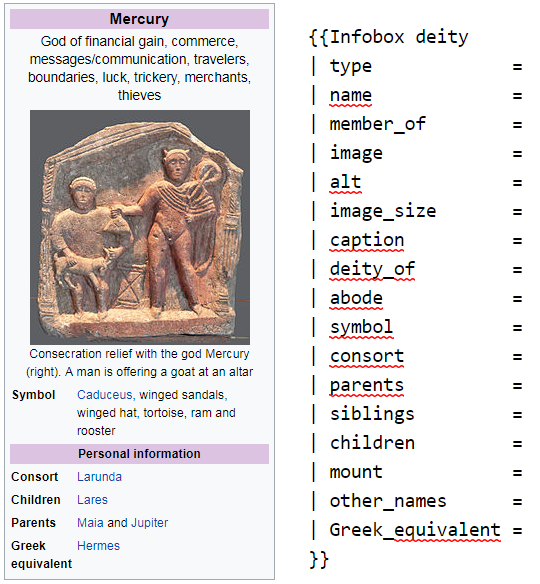
\includegraphics[width=0.8\linewidth]{mercury-infobox}
  \caption{Example Infobox of the page related to the god Mercury with the default properties for infoboxes about deities.}
  \label{fig:mercury-infobox}
\end{figure}



\subsubsection{\hspace*{3pt} Categories}

Every Wikipedia article should have at least one category. Categories are collections that identify topics in the encyclopedia. It should be noted that although the structure of the Wikipedia categories form a taxonomy, it is not represented by a simple tree of subcategories but, in fact, by a complex graph. This graph allows multiple simultaneous categorizations of topics, which means that one category may have multiple parents. The category "Semantics" is a good example of this complex structure since it is a subcategory of ``Grammar",  ``Linguistics", ``Concepts in logic", ``Semiotics", ``Philosophy of language" and others as demonstrated in figure \ref{fig:semantics-category}.


\begin{figure}[H]
\centering
  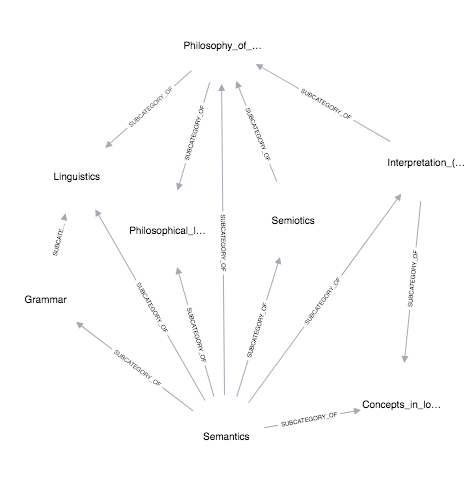
\includegraphics[width=0.8\linewidth]{graph-semantics}
  \caption{Example of an induced graph showing the supercategories of ``Semantics" in the Wikipedia Category Graph.}
  \label{fig:semantics-category}
\end{figure}

Although not based on semantics, Wikipedia has a set of characteristics, such as the definition of a large number of articles and organization of articles in categories, which make it an essential semantic resource. A simple example, but one that illustrates the complexity of the relationships between Wikipedia categories well, is the ``Apple" concept (the fruit), which is directly linked to four categories: ``Apples", ``Malus", ``Fruits originating in Asia", and ``Plants described in 1768". Each of these categories has been added and curated by people who are part of the Wikipedia community. In addition to the explicit knowledge in the directly attributed categories, a vast quantity of implicit knowledge can be inferred by the relations between them, both generically and specifically. Taking the category ``Apples'' as the starting point, links can be followed to the top of the classification system, in what can be perceived as a more generic case: Apples $\rightarrow$  Edible Fruits $\rightarrow$ Edible Plants $\rightarrow$ Food $\rightarrow$ Food and Drink $\rightarrow$ Health.
A more specific case can be illustrated by taking the ``Malus'' category as the origin, and analyzing one of the possible paths to the top: Malus $\rightarrow$ Maleae $\rightarrow$ Prunoideae $\rightarrow$ Rosaceae $\rightarrow$ Rosales $\rightarrow$ Rosids $\rightarrow$ Core Eudicots $\rightarrow$ Eudicots $\rightarrow$ Angiosperms $\rightarrow$ Plants $\rightarrow$ Eukaryota $\rightarrow$ Organisms $\rightarrow$ Life.
These are examples capture small fragments in Wikipedia's categorization structure for the ``Apple" concept. The complete structure involves 33 different categories and 42 different relations between them (See figure \ref{fig:semantics-category-apple}).


\begin{figure}[H]
\centering
  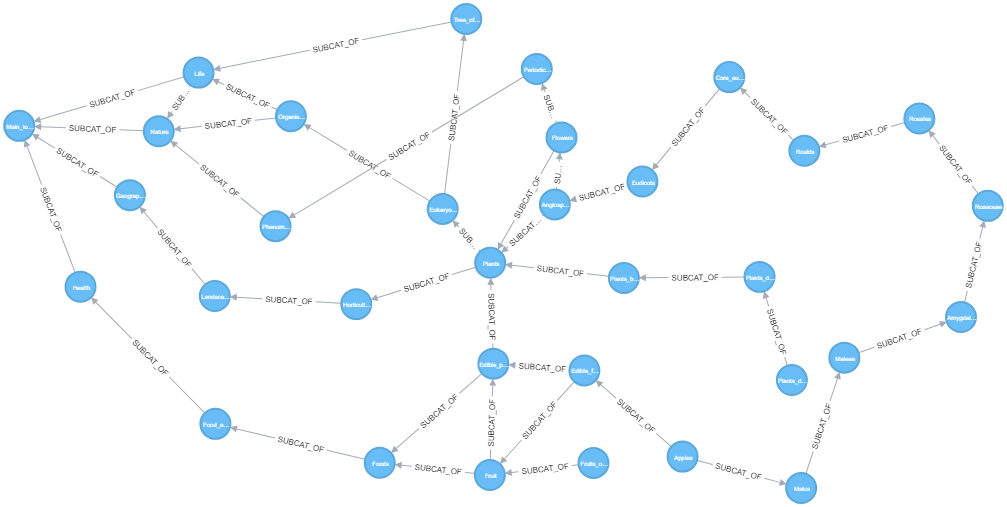
\includegraphics[width=0.8\linewidth]{graph}
  \caption{Example of an induced graph showing the categories and relationships for the Entity Apple towards Main topics}
  \label{fig:semantics-category-apple}
\end{figure}


%\subsection{\hspace*{3pt} DBpedia}

%As described directly on the DBpedia about page\footnote{url{https://wiki.dbpedia.org/about}} DBpedia is a crowd-sourced community effort to extract structured content from the information created in various Wikimedia projects. This structured information resembles an open knowledge graph (OKG) which is available for everyone on the Web. A knowledge graph is a particular kind of database which stores knowledge in a machine-readable form and provides a means for information to be collected, organized, shared, searched and utilized.

%The DBpedia dataset has many advantages compared to the raw data from Wikipedia. Besides the more convenient access to the underlying Wikipedia data sources, it also provides a higher data quality. The higher quality is because the extraction framework embeds multiple steps commonly found in data mining applications, such as duplicate removal in the form of mapping redundant infobox properties to the same DBpedia property.
%Therefore, the present work is focussed on using DBpedia for the entity named recognition and Linking, as well as for traversing entities' categories.

%\subsubsection{\hspace*{3pt} SPARQL}

%\gls{sparql} is a query language capable of retrieving and manipulating data stored in the \gls{rdf} format that is the basis of the OWL language. \gls{rdf} is a labeled and directed data format used to represent information on the Web \cite{prud2008sparql}. 

%In the context of this research, our approach exploits a small part of what the SPARQL language can provide. We navigate in the DBpedia hierarchy to retrieve broader semantic relations between the entities and its categories. 


\subsection{\hspace*{3pt} The Wikipedia Category Graph (WCG)}

Regarding the reduction of dimensionality, a proposed method consists of navigating the \gls{wcg} from each category extracted related to the entities obtained from the text-based resources towards the top of the graph, by all the shortest paths between the category and a set of top-level categories. 

The \gls{wcg} mentioned above is a set of almost 1,500 categories, describing a broad domain of knowledge and ranging from the very precise, such as ``Lists of Canadian network television schedules”, to the very general, such as ``information”. The categories are connected by hypernym relationships, with a child category having an ``subcategory-of” relationship to its parents in the direction of the relationship. However, the graph is not strictly hierarchic: shortcuts exist in the connections (i.e., starting from one child category and going up two different paths of different lengths to reach the same parent category) as well as loops (i.e., beginning from one child category and going up a path to reach the same child category again).

Given the complexity and dimension of the \gls{wcg}, a graph-theoretic analysis was carried out and is described in Chapter \ref{chapter:graph}. 

    \chapter{\hspace*{3pt} Topology Description of the Wikipedia Category Graph}
\label{chapter:graph}

The inspiration for this section comes from the work of Zesch and Gurevych\cite{zesch2007analysis}, where they showed that the \gls{wcg} is a scale-free, small-world graph, like other semantic networks such as WordNet or Roget’s thesaurus. They concluded that the \gls{wcg} could be used for \gls{nlp} tasks, where other semantic networks have been traditionally employed\cite{zesch2007analysis}.

Although their work has been useful in supporting many types of research in the recent years, the analysis was performed in a German Wikipedia version of 2007. The idea behind our updated review is to understand if the latest version of Wikipedia in English also presents the same characteristics. We also expect to obtain insights on how the structure of the \gls{wcg} can influence the proposed method and guide the development of future work. 



\section{\hspace*{3pt} Graph Density}

The Wikipedia Category Graph assembled for the experiments contains $1,475,806$ vertices and $4,091,417$ edges. Each vertex represents a category and each edge represents a relationship of the type ``Subcategory Of". 


The density $D$ of $G$ is the ratio of edges in $G$ to the maximum possible number of edges, defined in a directed graph as  
\begin{equation}
D={\frac  {|E|}{|V|\,(|V|-1)}}
\end{equation} where $V$ is the set of nodes and $E$ is the set of edges.

A graph is said to be dense when the number of existing edges is close to the number of possible edges. In the Wikipedia Category Graph the density is $1.878519 * 10^{-6}$.


\section{\hspace*{3pt} Degree Analysis}


If we observe a node in a directed graph, it is possible to see edges converging in the node and edges diverging from the node. An incoming edge and an outgoing edge can mean very different things, but in the Wikipedia Category Graph they both denote the direction of the relationship ``is a subcategory of". 

The indegree of node $v$ is the total number of connections onto node $v$.
On the other side, the outdegree of node $v$ is the total number of connections coming out from the node.

In both cases, the sum is the result of all other nodes $j$ in the graph. It is also possible to sum indegrees and outdegrees to get the total number of connections of a node, which constitutes its total degree.

The average indegree, outdegree and total degree for each vertex in the Wikipedia dataset are $2.78\pm0.142$, $2.78\pm0.001$ and $5.573\pm0.001$ respectively. 

\subsection{\hspace*{3pt}  Degree Distribution}

Large graphs such as the \gls{wcg} can be very complex structures, as the connections among the nodes can present complicated patterns. 
While studying complex networks, it is common to develop simplified measures that capture some elements of the structure. In this context, the degree distribution of a complex network is often described. 

The degree distribution of a graph is the probability distribution that a randomly chosen node will have a degree $k$. 

In directed graphs the degree distribution is a two-dimensional distribution, so that $P_{\text{deg}}(k^{\text{in}},k^{\text{out}} ) =$ the portion of nodes in the graph with indegree $k^{\text{in}}$ and outdegree $k^{\text{out}}$

Figure \ref{fig:in-and-out-degree} shows the degree distribution for the Wikipedia Category Graph in log-log\footnote{
A two-dimensional graph of numerical data that uses logarithmic scales on both the horizontal and vertical axes. 
} plot. The $x$-axis shows the degree while the $y$-axis shows the count of nodes with such degree. 

\begin{figure}[!h]
\centering
\begin{subfigure}{0.49\textwidth}
\centering
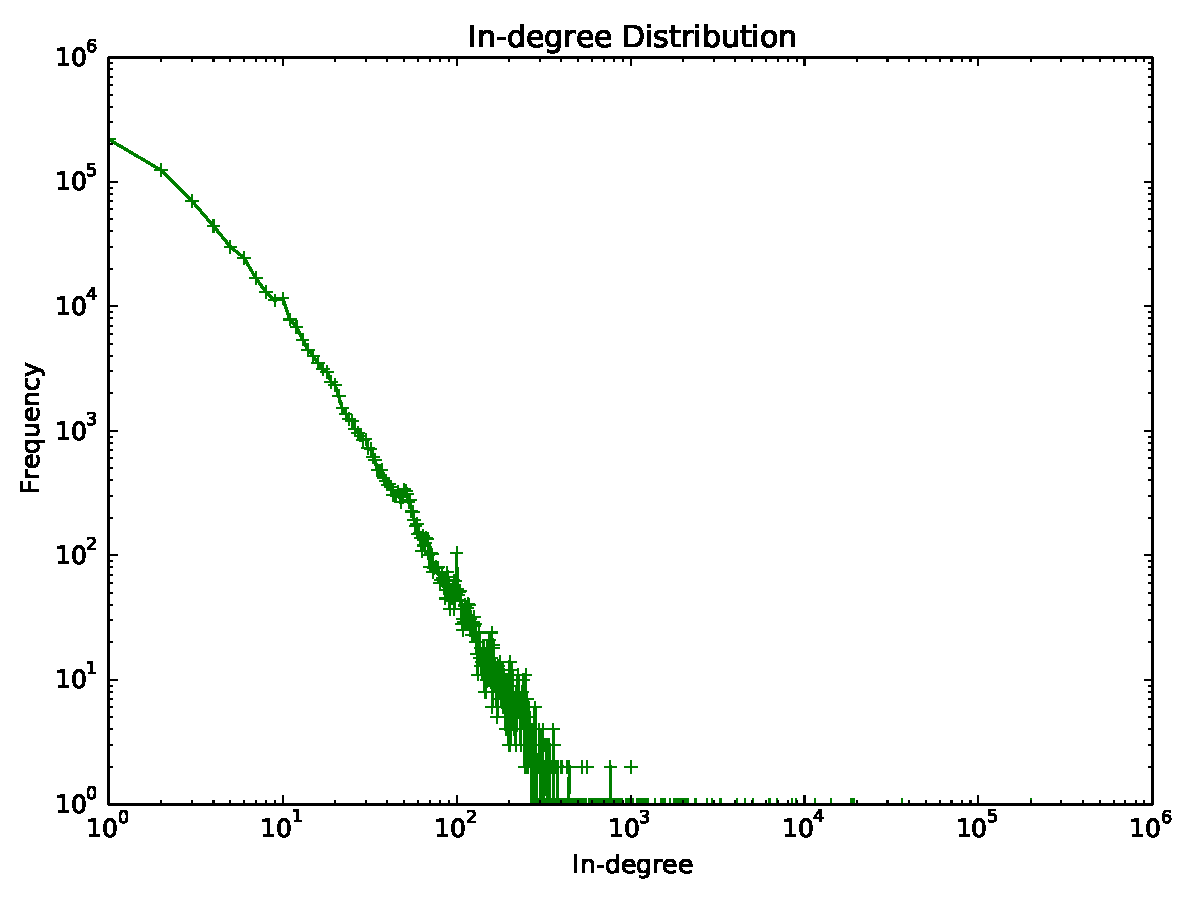
\includegraphics[width = \textwidth]{wikipedia-in-deg-dist.pdf}
\caption{Distribution of indegree}
\label{fig:left}
\end{subfigure}
\begin{subfigure}{0.49\textwidth}
\centering
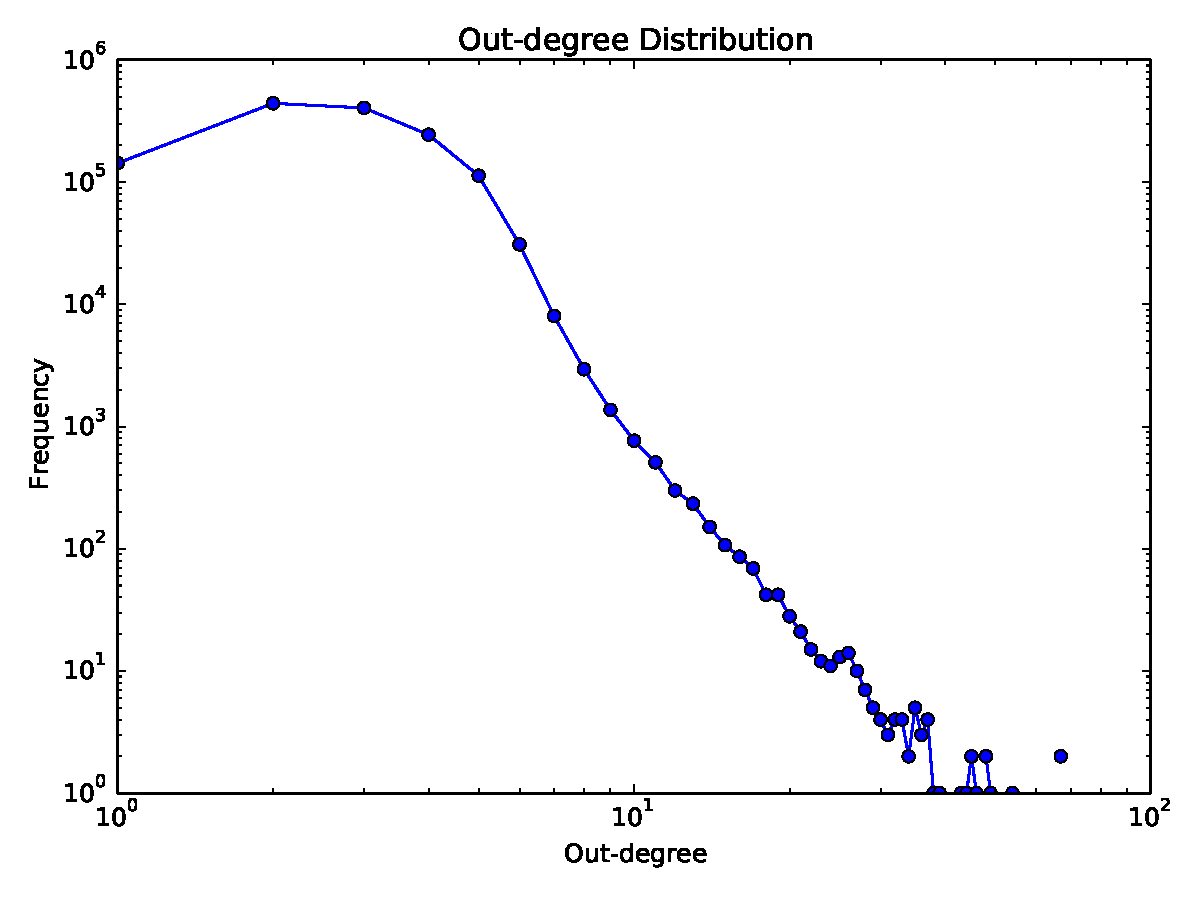
\includegraphics[width = \textwidth]{wikipedia-out-deg-dist.pdf}
\caption{Distribution of outdegree}
\label{fig:right}
\end{subfigure}
\caption{Indegree and outdegree distributions}
\label{fig:in-and-out-degree}
\end{figure}
Natural occurring networks tend to show a power-law distribution\footnote{A relationship between two variables such that one is proportional to a fixed power of the other.} which means that the fraction $P(k)$ of nodes in the graph having $k$ connections to other nodes varies as a power of some attribute $\alpha$, as in: 
\begin{equation}
P(k)=Ck^{-\alpha}
\end{equation}

This form of $P(k)$ decreases slowly as the degree $k$ increases, which multiplies the likelihood of finding nodes with a considerable degree.

Due to the fact that power-law networks do not have a typical degree, they are referred to as scale invariants or scale-free networks, which are characterized by the presence of large hubs\cite{mihalcea2011graph}. 

A method for determining the coefficient of the power law is defined in \cite{clauset2009power} as \begin{equation}
\alpha = 1 +n\left[\sum_{i=1}^n\ln\frac{x_i}{x_{\min}}\right]^{-1}
\end{equation}
where $x_{\min}$ is a lower cutoff, below which the power law cannot be observed. 


\begin{table}[ht!]
\centering
\begin{tabular}{@{}lll@{}}
\toprule
           & $\alpha$ & $x\_{min}$ \\ \midrule
in-degree  & 2,4124 & 10         \\
out-degree & 4,5603 & 12         \\ \bottomrule
\end{tabular}
\caption{Power-law parameters of the Wikipedia Category Graph}
\label{tab:power-law-params}
\end{table}

Based on the analysis of the \gls{wcg} degree distribution, as presented by the plot in figure \ref{fig:in-and-out-degree} and the exponent displayed in table \ref{tab:power-law-params}, it is demonstrated that the Wikipedia Category Graph nodes follow a power-law distribution, hence we can consider it as a scale-free network.  

A remarkable peculiarity of a scale-free network, derived from its degree distribution, is its tolerance to mistakes. If a random vertex is disconnected from the network, the highest probability is that this vertex has a low degree, causing a little impact for the interconnectivity of the remaining vertices.

\subsubsection{\hspace*{3pt} Assortativity}

Regarding the degree distribution in a graph $G$, we can also determine the assortativity coefficient $r$, which measures how vertices of different types are preferentially connected amongst themselves. The assortativity coefficient \cite{newman2003mixing} is the Pearson correlation coefficient of degree between pairs of linked nodes. Positive values of $r$ indicate a correlation between nodes of similar degree, while negative values indicate relationships between nodes of different degree. In general, $r$ lies between -1 and 1. When $r = 1$, the network is said to have perfect assortative mixing patterns, when $r = 0$ the network is non\-assortative, and when  $r=-1$ the network is completely disassortative.

The assortativity coefficient for our graph for indegree, outdegree and total degree are  respectively: 
$-0.0034$, $0.0898$, $0.0051$. 

Assortativity is high when high-degree nodes tend to connect to other high-degree nodes, and it is low (i.e., negative) when high-degree nodes are linked to low-degree nodes. An assortativity of 0 indicates no correlation between the degrees of the nodes.

In this case, since the assortativity regarding indegree and outdegree is very low, we can infer that there is no preferential attachment in the \gls{wcg}, meaning that nodes with a high degree will not necessarily be connected to other nodes with high degree.  Hence, the hubs are distributed along the structures and not concentrated in a same region of the graph.


\subsection{\hspace*{3pt} Path lengths}

A path in a graph is a sequence of alternating nodes and edges that starts with a node and ends with another node in such a way that adjacent nodes and edges in the sequence are incidental to each other \cite{newman2010networks}. Nodes or edges can appear in the same path multiple times, and the number of edges in a path is the length of that given path. If a graph is connected, then any node can be reached via a finite-length path starting from any other node. The shortest path between a pair of nodes is called a geodesic path and there can be more than one such path.

The average path length, a concept in the field of network topology, is defined as the average number of steps in the shortest paths for all possible pairs of nodes in the graph. In directed graphs, the average path length is calculated as follows:

\begin{equation}
l_{G}={\frac  {1}{2 * n\cdot (n-1)}}\cdot \sum _{{i\neq j}}d(v_{i},v_{j})
\end{equation}

where $d(v_{1},v_{2})$ denotes the shortest distance between $v_1$ and $v_2$ and $n$ is the number of vertices in the graph $G$. 

If two nodes are disconnected (i.e., no path exists between them), the path length between these nodes is infinite. Consequently, if a graph contains disconnected components, the average shortest path length $l_G$ tends to infinity. 
Given that the \gls{wcg} is not completely connected, to avoid infinity, we calculated the average shortest path length for the largest connected component. As a result, the $l_G$ is $20,9343$. The shortest path length distribution is displayed in figure \ref{fig:path-distribution} where the y-axis represents the number of nodes and the x-axis represents the number average path length.



\begin{figure}[H]
  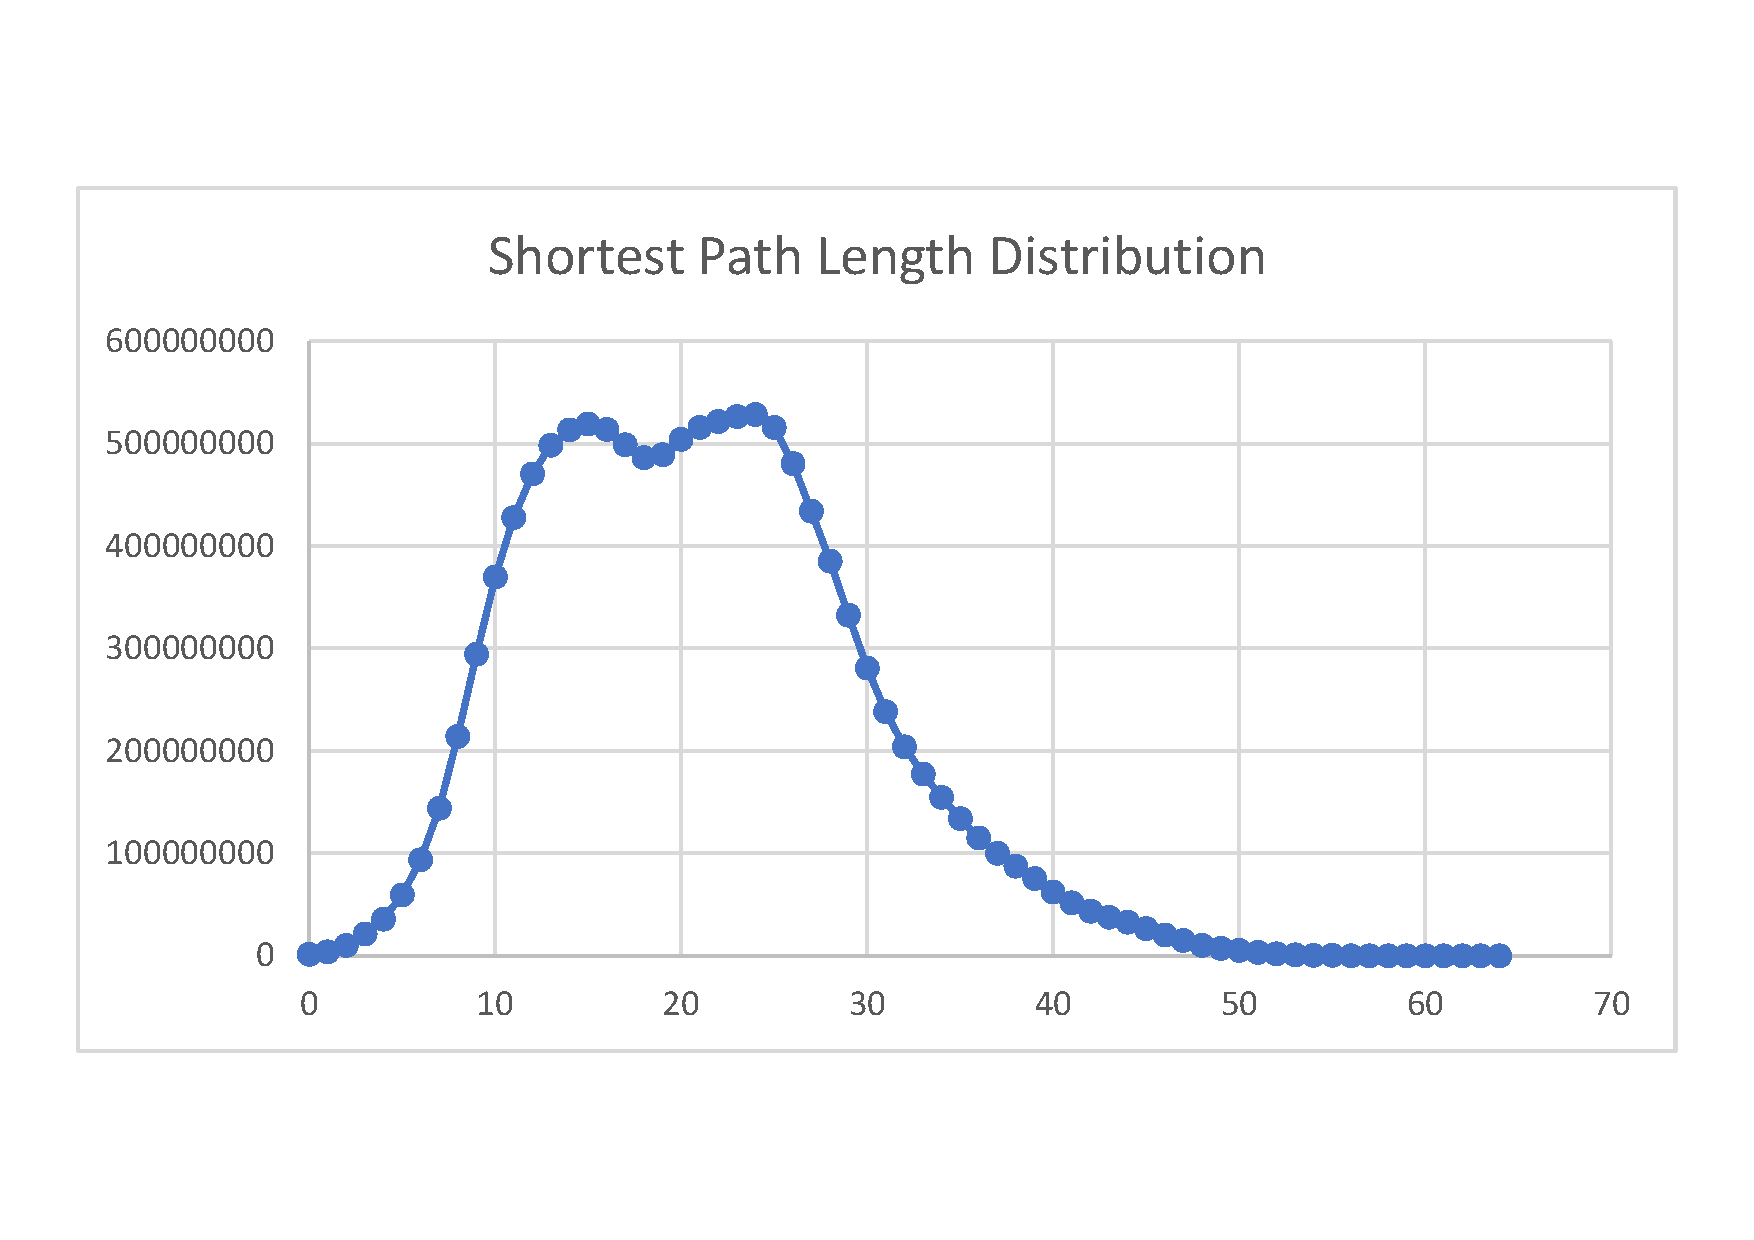
\includegraphics[width=\linewidth]{path_frequency2}
  \caption{Shortest path length distribution on the Wikipedia Category Graph}
  \label{fig:path-distribution}
\end{figure}


\subsubsection{\hspace*{3pt} Graph Diameter}

The diameter $d$ of a graph $G$ is the maximum topological distance that can be found between two nodes in $G$. In order to find the diameter of a graph, the shortest path between each pair of vertices needs to be determined first. The greatest length of any of these paths is the diameter of the graph. Alternatively, we can define it as 
\begin{equation}
d=\max _{v\in V}\epsilon (v)
\end{equation}
It is worth noticing that the distance is determined based on the graph direction. In the Wikipedia Category Graph, the maximum topological distance is $52$ and the nodes with the longest shortest path are Bengali Culture and Politics of Bangladesh. 


\subsection{\hspace*{3pt} Small World}

A small-world is a type of graph in which most nodes are not neighbors between them, but the neighbors of any given node are likely to be neighbors of each other, and most nodes can be reached from every other node by a small number of steps. Specifically, a small-world network is defined to be a network where the typical distance $L$ between two randomly chosen nodes grows proportionally to the logarithm of the number of nodes $N$ in the graph $G$ while the clustering coefficient is not small.

Formally, a graph $G$ with $n$ nodes and $m$ vertices is said to be a small-world if it has a similar path length but greater clustering of nodes than an equivalent Erdös-Rényi (E–R) random graph with the same $m$ and $n$. Let $L_g$ be the mean shortest path length of $G$ and $cc_{2_g}$ its clustering coefficient using the equation \ref{eq:cc2}. Let $L_{rand}$ and  $cc_{2_{rand}}$ be the corresponding quantities for the corresponding E–R random graph. According to the empirical experiments performed in \cite{watts1998collective}, a graph $G$ is said to be a small-world network if $L_g \ge L_{rand}$ and $ cc_{2_g} \gg cc_{2_{rand}}$.

In small-world graphs, the distance between any pair of nodes is relatively short while the level of transitivity, or clustering. is relatively high.


Another important metric for understanding the topology of a graph is its clustering coefficient. The clustering coefficient of a vertex represents the probability that if two of its neighbors are randomly chosen, they will also be connected by an edge. More precisely, if a vertex has $t$ neighbors, then there are $t(t-1)/2$ possible edges that connect those neighbors. The local clustering coefficient of a vertex is the fraction of the edges that actually appear in the graph (or 0 if the vertex has degree 0 or 1). Given the graph $G= (v,E)$ and a vertex $v \in V$, the clustering coefficient of $v$ is 

\begin{equation}\label{eq:cc1}
cc_1(v) = \dfrac{number of pairs of neighbors connected by edges}{number of pairs of neighbors}  
\end{equation} 

The clustering coefficient of a graph $G$ is the average of the local clustering coefficients $cc_1(v)$ of all vertices $v \in V$. The Wikipedia Category Graph has a clustering coefficient of $0.0461$. 

An alternative way of calculating the clustering coefficient of a graph is referred to as the global clustering coefficient or transitivity \cite{newman2001random}. Given the graph $G = (V,E)$ the global clustering coefficient of $G$ is
\begin{equation}\label{eq:cc2}
cc_2 = \dfrac{number of closed 2paths}{number of 2paths}
\end{equation} For the Wikipedia Category Graph, the global clustering coefficient is $0.0036\pm0.005$. 



\begin{table}[!h]
\centering
\begin{tabular}{@{}lllll@{}}
\toprule
    & $L_g$       & $L_{rand}$       & $cc_{2_g}$           & $cc_{2_{rand}}$        \\ \midrule
WCG & 20,9343 & 19,5389 & 0,003638604 & 2,03E-06 \\ \bottomrule
\end{tabular}
\caption{Empirical demonstration of small-worldness of WCG }
\label{small-worldness}
\end{table}

Therefore, the Wikipedia Category Graph exhibits a small-world behavior, with an average shortest path length close to that of a random network with the same size.



%Most real-world networks, however, especially social networks, do not have homogeneous distribution of degree that regular or random networks have. The number of connections each node has in most networks varies greatly and they are positioned somewhere between regular and random networks. In fact, Watts and Strogatz (1998) proposed a model where the connections between the nodes in a regular graph were rewired with a certain probability. The resulting graphs were between the regular and random in their structure and are referred to as small-world (SW) networks. SW networks are very close structurally to many social networks in that they have a higher clustering and almost the same average path than the random networks with the same number of nodes and edges. SW networks usually have high modularity (groups of the nodes that are more densely connected together than to the rest of the network). The graph above shows a different type of a SW network though, the one that’s generated by rewiring the connections from within the interconnected modules to between these modules – an architecture that is often found in cortical maps (neural networks in the brain).

%Finally, there’s a large class of so-called scale-free (SF) networks characterized by a highly heterogeneous degree distribution, which follows a ``power-law” (Barabasi & Albert 1999). They are called scale-free, because zooming in on any part of the distribution doesn’t change its shape: there is a few, but significant number of nodes with a lot of connections and there’s a trailing tail of nodes with a very few connections at each level of magnification. Such networks are typical for the structure of the world wide web, semantic maps, electronic circuits. These structure combine heterogeneity and randomness, they can have low or high modularity and many SW networks are also scale-free.

    \chapter{\hspace*{3pt} Fundamental Concepts}
\label{chapter:related-concepts}



This chapter introduces the theoretical concepts used to contextualize the research described in this thesis.

The concepts related to Collective Intelligence and Collective construction of Knowledge are essential for understanding the motivation to choose an approach that uses the knowledge of the contributors of Wikipedia, rather than experts. The description of Wikipedia and its features is central to the understanding of the organization of this body of knowledge, as well as the possibilities and challenges that emerge from decoding  the underlying structure. 
The concepts related to Information Retrieval and Extraction are essential to understanding the tasks applied in the proposed solution to extract the entities and the categories from the text-resources.
We also provide some general information about natural language processing (NLP) techniques that are applicable to our categorization method. 
This chapter ends with an overview of the concept and methods for the automatic classification of textual resources, as it is the primary goal of the research presented in this thesis. 

\section{\hspace*{3pt}Natural Language Processing - NLP}


\gls{nlp} consists of the development of mathematical and computational models of various aspects of language, to make possible the development of a wide range of systems that rely on information expressed in natural language \cite{joshi1991natural}.

Natural language is any language developed naturally by the human being, in an unpremeditated way, as a result of the natural ease of language processing by the human intellect \cite{chomsky1975logical}. Spoken, written and sign languages are examples of natural languages. 

\gls{nlp} has the general objective of processing human language so that it is understandable by the computer. Among the essential areas of \gls{nlp} we can highlight: the recognition of voice, the recognition of writing and the reproduction of voice from the text. \gls{nlp} encompasses several and complex areas of knowledge, hence the  researches in this field are interdisciplinary, involving concepts of computer science, linguistics, logic, and psychology.

One of the uses of \gls{nlp} is the extraction of meaning from unstructured resources so that they can be used in a structured way in computational application.

Structured resources are machine-readable resources that encode relationships of various types according to the level of information \cite{hovy2013collaboratively}. Structured resources are of high quality as they are built from the knowledge of domain experts, lexicographers, and linguists. However, structured resources are limited because they require significant efforts in creation and updating. Because they are built manually, they depend on the availability of experts to extend their coverage and to keep them up to date on recent events. Moreover, knowledge encoded in one language is not transferable to others, requiring a new effort for each new language.

The most common structured resources are:

\begin{itemize}

\item Thesaurus: collections of related terms;
\item Taxonomies: Hierarchical structures of classification of terms;
\item Ontologies: knowledge models that include concepts, relations of different types, rules and axioms.
\end{itemize}

Unstructured resources are collections of texts that have no formalized knowledge and are machine readable only as sequences of characters and words. Different statistical models can extract knowledge from unstructured collections, and the massive amount of texts available on the \gls{www} enables the construction of knowledge bases of excellent coverage. However, they are limited by the lack of texts that demonstrate common-sense knowledge \cite{hovy2013collaboratively}. Also, statistical models are not able to issue knowledge with quality equivalent to the resources built by specialists.

The limitations of unstructured resources are complementary to the limitations of structured resources. While unstructured resources enable broad coverage with low quality, structured resources have high quality but low coverage. Semistructured resources constructed collaboratively on the \gls{www} encode the knowledge voluntarily made available by users of these resources, covering different areas of knowledge and having quality comparable to that obtained from specialists. The semi-structured resources mentioned by the authors are Wiktionary, Flickr, Twitter, Yahoo! Answers and, with greater emphasis on the Wikipedia \cite{hovy2013collaboratively}.

Nowadays, most of the information in government, industry, business, and other institutions are stored electronically on the Web, in the form of semi-structured or restructured resources.



In this context, the existence of \gls{ir} systems becomes indispensable to assist users in the process of locating information that is relevant in collections of unstructured or semi-structured data (e.g., web pages, documents, images, video, etc.).  


\section{\hspace{3pt}Information Retrieval}

\gls{ir} systems are mostly known for their searching ability, where a user states an information need and the system provides the user with a response to this information need in return. \gls{ir} is a large academic field and encompasses several topics like browsing or filtering documents, processing of retrieved documents and clustering or classifying documents according to their content \cite{Manning:2008}, Manning defines \gls{ir} as finding material (usually documents) of an unstructured nature (usually text) that satisfies an information need from within large collections (usually stored on computers).

A system can increase its precision when retrieving the users' information need if it indexes well-representing features of the text. As the collection of documents expand, automatic techniques that can extract these features become crucial.  \gls{tc} techniques can provide an output that can be representative of a research document, allowing for \gls{ir} systems to handle the indexing and retrieval process.



\section{\hspace*{3pt}Information Extraction}

\gls{ie} is the process of automatically extracting particular information entities or the relationship between different information entities from a source \cite{sarawagi2008information} and presenting it in a structured form. The source of information can be structured like a relational database, semi-structured like an HTML document or unstructured as free text from an academic paper. IE combines techniques from \gls{nlp}, lexical resources and semantic constraints to effectively provide automatic mining of documents.

\subsection{\hspace*{3pt}Documents Representation}

Document representation has substantial importance when dealing with text classification.

Plain texts are usually not used directly by classification algorithms.  The documents are processed and transformed so that they can represent the semantic content of the text optimized for numeric processing.   

Most \gls{tc} methods use the \gls{bow} approach to represent documents. \cite{Lan:2009} \cite{Manning:2008}. The categorization takes into account the presence or the absence of key terms in the document-terms matrix that represents each document, as stated by Sebastiani \cite{Sebastiani:2002}.

The reasons for using this approach is the simplicity, efficiency and relative effectiveness of the \gls{bow} paradigm.

However, the \gls{bow} method fails to take into account relevant aspects of the text that is being represented. Semantic relationships between key terms are ignored, as well as the order in which the terms appear \cite{Gabrilovich:2005, Lan:2009}.

As a consequence, if two documents use different sets of keywords to describe the same topic, they can be classified as being of different categories, even though the keywords used by both are probably synonymous or semantically associated in some other form \cite {Hu:2009}.

Amidst the alternative representations that use features of the text itself, most commons are those that use sequential co-occurrence of n terms (n-grams) and non-sequential co-occurrences of n terms (termsets). 

Other approaches have explored features that are not directly extracted from the text. As an example, we can mention the growing interest in \gls{fg} techniques known as Document Expansion or Document Enrichment, through which new terms are added to documents, enhancing the \gls{bow} representation by inserting more information in the document-term matrix \cite {Gabrilovich:2005}.

Numerous methods that use Feature Generation have achieved excellent results in Text Classification through the extraction of semantic relations such as synonymy, hyponymy and associative relations between concepts, present in Encyclopedias, Thesaurus, Ontologies, Web Pages and other sources. \cite{Gabrilovich:2005,Gabrilovich:2006,Hu:2008,Wang:2008, Wang:2009}.


\subsection{\hspace*{3pt}Features Representation}

Terms, also called features\cite{Sebastiani:2002}, are indexable units used to identify the contents of the text document, and can be described at various levels of granularity, such as syllables or word (uni-grams ); several words (bigrams, trigrams or n-grams); phrases, or any other more elaborate semantic or syntactic unit \cite{Lan:2009}.

The most commonly used feature representation TC is known as a set of terms representation or also as \gls{bow}, and considers only the words present in the text as terms.
 
However, this approach ignores essential semantic relations between the terms \cite {Hu:2008}.
In fact, elements like ``White House" or ``Bill Gates" are represented in the BOW as unrelated words. In analyzing the BOW representation of a given document in which the words Bill and Gates occur, one might suggest that the document talks about accounting, regarding the word Bill or construction because of the word Gates. For a computer program, it would be challenging to associate both words.
Nevertheless, if the representation of the same document contains the set of words ``Bill Gates" as a term, it would be easier for the classifier to make a correct association.\cite{bekkerman2004using}.



\subsection{\hspace*{3pt}Named Entity Recognition and Linking }


Grishman and  Sundheim \cite{grishman1996message} defined the task of \gls{ner}, as the task ``which involves identifying the names of all people, organizations and geographic locations in a text," also involving the identification of date expressions, hour, monetary values and percentages. 


The named entity recognition task has been researched under several names over the years. For example Wikification \cite{Ratinov:2011}, Grounding \cite{leidner2003grounding} or Named-entity disambiguation \cite{hoffart2011robust}. The common approach can be generalized into following steps: find named entity mentions in given text, generate a set of candidates for each mention, select the best candidate for each mention, link the mention to the corresponding entry on Knowledge Base.

In its most common form, the \gls{ner} task recognizes a predefined number of semantic categories, such as those defined in \cite{grishman1996message}. However, it has also been successfully applied to specific domains such as biology \cite{campos2012biomedical} and geology \cite{sobhana2010conditional}, where a more substantial number of domain-related categories are used. A prevalent form is the use of linguistic rules for the recognition of entities. In this approach the rules are manually coded from grammatical and domain knowledge, requiring specialization in both to obtain good results \cite{nadeau2007survey}. Moreover, the use of linguistic rules restricts its use to documents written in the language for which the rules were codified, making it impossible to use them in other languages.

Another conventional approach to \gls{ner} is through the use of \gls{ml}.

The algorithms must be trained with previously annotated texts so that they learn through these annotations on how to identify if a specific sequence of words belongs to one of the categories annotated. 

The annotations identify for each word in the text what it the grammatical class. If the word is an entity name, it identifies its type. The \gls{ner} in a text goes through two phases: ii) the annotation of the grammatical classes of the text; and ii) the annotation of the names with the semantic category.

The quality of the algorithm depends on the annotator's ability to identify the names correctly and is limited to the types of entities used in the corpus. 

Supervised machine learning algorithms are expected to be able to generalize features found in the training text - known as Gold Corpus - in the form of patterns that when identified in other texts lead to the correct classification of entities. 

For an algorithm to be able to learn these patterns it needs a large and diverse enough corpus. The size of the corpus interferes because the algorithm needs repetitions of a pattern to be able to recognize it. 

According to Domingos \cite{domingos2012few}, diversity in training sets is necessary because if the algorithm is exposed to a substantial number of occurrences of the same pattern, it will not be able to identify small variations in this pattern and will not be able to differentiate classes with similar features.

Ratinov and Roth \cite{Ratinov:2009} argue that \gls{ner} is a sequential prediction problem, solvable with typical models for this class of problems such as Hidden Markov Models, Conditional Random Fields, and Perceptrons.



\section{\hspace*{3pt}Automatic Text Classification}

Based on Sebastiani\cite{Sebastiani:2002}, the automatic classification of documents through \gls{ml} approach requires the availability of an initial corpus  $\Omega=\{d_1,d_2, \cdots, d_{|\Omega|}\} \in D$ documents manually classified by a specialist, in a set of categories $C =\{c_1, c_2,\cdots c_{|C|}\}$. Thus, the result of the classification function for the objective $\Psi: D × C \mapsto \{T, F\}$ has its known values for every pair $(d_j, c_i) \in \Omega × C$

The classification function $\Phi: D × C \mapsto \{T, F\}$ is derived from the learning process. This function maps documents into classes and is commonly called a classifier. Thus, the classification task seeks to approximate as much as possible the classification function $\Phi$ with the unknown value of the objective function $\Psi: D × C \mapsto \{T, F\}$ so that the result of $\Phi$ and $\Psi$ are similar. It is necessary to evaluate the effectiveness of the classifier by comparing the results obtained with the expected results of the function $\Psi$.

In order to perform the training and evaluation of the classifier two distinct subsets of $\Omega$, $T_v$ and $T_e$, such that $T_v \cap T_e = \emptyset$:



\begin{itemize}
\item \textbf{Training Set $T_v$} - used to derive the classifier Φ. The classifier is trained in learning the features of the training set which has already been manually classified.


\item \textbf{Test Set $T_e$} - used to evaluate the efficiency of the classifier $\Phi$. The class (or classes) assigned to each document $d_j$ belonging to the test set is previously known. This information is not taken into account by the classifier $\Phi$ created in the training stage. Each document $d_j  \in T_e$  is submitted to the classifier $\Phi$ which assigns one or more classes from $C$ to $d_j$, comparing the features present in $d_j$ with the features learned during the training stage.
\end{itemize}


The next step is the evaluation of each decision made by the classifier
Φ for each pair $(d_j, c_i)$, which is compared with the expected decision $\Psi(d_j, c_i)$. The higher the number of decisions of $\Phi$ that are equal to the decisions of $\Psi$, the more effective is the classifier.

A classifier $\Phi$ must have a good generalization capability, in order to eliminate errors caused by over-fitting. This problem occurs when a classifier adapts itself to particular features of the training documents, which can decrease the correctness rate for the classification of new
documents.

The methods that are used in \gls{tc} are frequently the same used in the more general area of \gls{ir}, where the goal is to find documents or sections within documents that are related to a particular query. \gls{tc} methods are essential to finding relevant information in many different tasks that deal with large volumes of text-based information. Some of the most traditional tasks where these methods are applied are: finding Internet pages on a given subject; finding answers to similar questions that have been answered before; classifying news by subject or newsgroup, among others. In each case, the goal is to assign the appropriate category or label to each document that needs to be classified.




%The process of evaluating classifiers will be discussed further in  in the section \ref{sec:evaluation-of-classifiers}.

\subsection{\hspace*{3pt}Types of Classification}

Depending on the approach, the classification method can assign one class or more than one class to the documents. 

If a document  $ d_j \in \Omega $  is assigned to only one class, it is called single-label, and when any number of classes from 0 to $|C|$ can be assigned to a document $d_j \in \Omega$, it is called multi-label. A single-label text classification problem can be further categorized into a  binary classification problem if only one class is assigned to the document.The single-label text classification problem becomes a multi-class problem if only N mutually exclusive classes are assigned to the document. 

The binary approach is said to be a more general approach than the multi-class approach since binary classification can be employed in multi-class classification problems.  To make it possible, it is needed to transform a multi-class classification problem, with documents $(c_1, \cdots, c_{ |C|})$, in $|C|$ independent problems of binary classification over $c_i$ or $\overline{c_i}$, with $i=1,\cdots,|C|$. In this case, $\overline{c_i}$ is formed by documents that belong to all other classes and this methodology is named \textit{one against others}. This solution is only possible when the classes involved in the problem are stochastically independent, meaning that the classification of a document into one class does not require that the same document is also categorized in another one.


\subsection{\hspace*{3pt}Text Classifiers}
\label{sec:text-classifiers}

Over the last few years, a vast number of algorithms have been proposed for \gls{tc} using machine learning. Among them, one can cite the naive Bayes \cite{mccallum1998comparison}, \gls{knn} \cite{Rijsbergen:1979}, \gls{svm} \cite{joachims1998text} and rule learning algorithms \cite{slattery1998combining}, which have been widely used. The researches that deal with document classification usually report performance comparison among the different algorithms available.




\section{\hspace*{3pt} Collective Knowledge Construction}

Pierre Lévy~\cite{levy1997collective}, a French philosopher who specializes in the understanding of the cultural and cognitive implications of digital technologies and the phenomenon of human collective intelligence, argues that knowledge is in humanity, and every individual can offer knowledge.

The cyberspace allows individuals to remain interconnected regardless of their geographic location. It deterritorializes knowledge and supports the development of collective intelligence. With regard to the efficient mobilization of competences, the author has stated that an essential factor is to identify and understand the capabilities of the subjects in their individualities. The project of collective intelligence, described by Lévy is not only linked to cognition.  It is also a global project that presumes practical actions intended to mobilize the competences of individuals to provide mutual recognition and enrichment of those who are involved in this proposal ~\cite{levy1997collective}.

Therefore, Lévy ~\cite{levy2001cyberculture} defines collective intelligence as a new sustainable way of thinking through social connections that become viable through the use of a network of people on the Web. This collective intelligence is distributed and coordinated in real time, which results in an efficient mobilization of skills, and the cyberspace favors its development.

\section{\hspace*{3pt} The Wikipedia}


Wikipedia is the most substantial encyclopedia freely available on the Web. It has been developed and curated by a large number of users over time and represents the result of a process of collective construction about facts, people and the broadest type of topics currently found on the Web.

Wikipedia content is available in around 300\footnote{\url{https://en.wikipedia.org/wiki/List_of_Wikipedias}} active languages. In the English version, it has more than 5.4M articles,  written and edited by a total of about 30 million registered editors of whom roughly 120,000 are currently active. In the last ten years, there has been a consistent average of 30 million edits per year, which includes both the creation of new articles and development of existing ones. 

This online encyclopaedia was created in January 2001 as an improvement of Nupedia, a free encyclopedia written only by specialists with rigid evaluation criteria, which had low adherence and was suspended in 2003.
Both Wikipedia and Nupedia projects were initiatives by Jimmy Wales and Larry Sanger. At the beginning of 2008, Wikipedia exceeded 8 million entries in 253 languages, doubling the number of entries each year during the following years, making it the 5th most accessed site in the web, according to the Alexa page\footnote{\url{www.alexa.com}}.

The success among users and its dissemination as a source of reference do not lie in the fact that Wikipedia is on the Internet since there are others alternatives available online. What differs is the possibility of participation, collaboration and collective construction. 


The Wiki system allowed not only the gathering of data but also the generation of new knowledge in a collective way between different subjects. In this regard, Wikipedia is not merely a tool for indexing and formatting but a space for debating and synthesizing texts. The contributors are not just ``librarians", but indeed authors, in the strictest sense of the word.  Hereof, Wikipedia is more than a source of information; it is also an invitation to the collaborative work towards knowledge construction. While the use of a conventional encyclopedia implies in querying for information that becomes dated at the time of its publication, and whose volumes rest immutable on the shelf, Wikipedia opens its pages to the present and the ongoing debate over available writings. Each participant contributes by offering questions for discussion. Through these mutual exchanges, the text of the entries is being discussed and improved. When text is compromised by the inclusion of dubious information, new discussions and corrections can be initiated.
Some authors have shown that vandalism and inaccuracies in Wikipedia are often reverted within a matter of minutes ~\cite{kittur2007he} ~\cite{viegas2004studying}.

A study by Wilkinson \& Huberman ~\cite{wilkinson2007assessing} indicated that the popularity of the project and the reliability of many of the texts is a result of the intense participation of registered users.
The thousands of volunteers who contribute to the project make the site an environment of intense social interaction, in which each user fulfills specialized functions, according to their interest, availability and eventually the bureaucratic role occupied in the Wikipedia project. 


Seeking to increase the reliability of content built in a collective and collaborative environment, Wikipedia has created a rigid organizational structure. 

Note that, as Tapscott and Willians \cite{tapscott2008wikinomics} affirm, collaborative production mixes elements of hierarchy and self-organization and is based on meritocratic principles of organization.

The editing community enforces specific codified rules designed to ensure accuracy and prevent bias in articles. A study comparing the efficiency of various scientific subjects in Wikipedia and Encyclopaedia Britannica found that while imprecisions were not infrequent, they occurred at similar rates between the two ~\cite{giles2005internet}. In particular, a Wikipedia science article contained an average of four mistakes, while an Encyclopaedia Britannica article included only three. 
As a matter of fact, Encyclopaedia Britannica currently has about 65,000, while English Wikipedia has approximately 5.4 million articles totaling 1.8 billion words. 


The Wikipedia is a free and online encyclopedia where all readers can update their content by including and editing their articles. Instead of following a peer review process by experts, Wikipedia articles are available for revisions and enhancements by readers. In his bibliographical review on the use of Wikipedia in Computing Science researches,  Wikipedia is a  valuable resource with broad functionalities.  In \cite{medelyan2009mining} it is demonstrated how researchers had developed sophisticated techniques for extracting knowledge from different perspectives:



\begin{itemize}
\item Wikipedia as an Encyclopaedia; 


\item Wikipedia as a corpus; 
\item Wikipedia as a thesaurus; 
\item Wikipedia as a database; 
\item Wikipedia as an ontology; 
\item Wikipedia as a graph


Even though Wikipedia texts are written in natural language, some structured resources are available for organizing the articles into categories, for connecting different articles, as well as for presenting relevant properties of the topic described in the article.

\end{itemize}
\subsection{\hspace*{3pt}Wikipedia Structure}

Wikipedia has different types of elements in its structure: articles, redirect pages, disambiguation pages, hyperlinks, categories, infoboxes, and Wikilinks. 

\subsubsection{\hspace*{3pt}Titles}
Each Wikipedia article has a name, which is the most common form of identification of the concept or entity described in the article.  People, organizations, places, events, and species of living beings are common classes described on Wikipedia. The titles are unique identifiers within the set of Wikipedia articles for a language.

\subsubsection{\hspace*{3pt}Wikilinks}

The guarantee of the uniqueness of the title makes it possible to reference an article through its title. Wikipedia explores this possibility through internal links (Wikilinks).   Wikilinks are references that enable navigation between articles in a network of internal links built by the publishers of the articles. 

Wikipedia recommends that editors link only the first occurrence of a reference to another article through a Wikilink. 

It is also possible to separate the link itself from the term it refers to, thus creating an alternative arbitrary text for the link. This process is often used for homonyms and abbreviations and can be applied by adding a pipe "|" divider followed by the alternative name. The article comes before the divider and the text that is displayed and placed after it.  For example, if we format a link like [[List of Presidents of the United States| 44th President of the United States]] the final article will display only the 44th President of the United States in the text and it will be a clickable link leading to the List of Presidents of the United States article on Wikipedia. 

\subsubsection{\hspace*{3pt}Disambiguation}

In many languages, it is common that a single word represents different concepts or entities (homonymous), which would violate this restriction of uniqueness for Wikipedia titles. In these cases, the article that defines the most known concept remains with the simple name, and the other titles must have a suffix for disambiguation. The suffix of disambiguation must present a detail that makes possible the differentiation of one article from the others. It is suggested that editors create a specific disambiguation page that lists the different homonymous articles with internal links to their contents. When it is not possible to determine which of the concepts is best known, the disambiguation page has the simple title, and all other pages have the suffix for disambiguation.


An example of disambiguation on Wikipedia in English is the concept ``Mercury" (see figure \ref{fig:mercury-desambiguation}, which can mean:

 \begin {itemize}
 \item A metallic chemical element with the symbol 'Hg.'
 \item A Roman god
 \item The first planet from the Sun
 \end {itemize}


 In this example, since it is not possible to determine the most known entity,  the disambiguation page has the title ``Mercury" \footnote{\url{https://en.wikipedia.org/wiki/Mercury}}, The planet has the title ``Mercury (planet)"\footnote{\url{https://en.wikipedia.org/wiki/Mercury_(planet)}}, the god has the title ``Mercury (mythology)"\footnote{\url{https://en.wikipedia.org/wiki/Mercury_(mythology)}} and the element is named ``Mercury (element)"\footnote{\url{https://en.wikipedia.org/wiki/Mercury_(element)}}.

\begin{figure}[!h]
\centering
  
\includegraphics[width=\linewidth]{desambiguation}
  \caption{Disambiguation page for the term ``Mercury"}
  \label{fig:mercury-desambiguation}
\end{figure}


\subsubsection{\hspace*{3pt} Redirects}

Another variant of Wikilinks is the redirect, employed when different textual forms know a concept or entity. This situation would conflict with the restriction of the uniqueness of titles, imposing the repetition of the content of an article with different titles. 

The redirect pages contain only text in the form of a directive without gender, number, or case. The central purpose is to find a single article for equivalent terms. For example, if the user searches for ``apples," the redirect page will refer them to the ``apple" article. 

Redirections also occur with people names, when they are known both by their full name and by part of their name or surname. It is the case of the English writer  J. R. R. Tolkien, well-known only by his last name, Tolkien.

\subsubsection{\hspace*{3pt} Infoboxes}

According to Wikipedia documentation\footnote{https://en.wikipedia.org/wiki/Help:Infobox}, infoboxes are fixed-format tables that summarize relevant aspects of an article. It is an optional feature, but they present common attributes between different subjects. Wikipedia recommends the use of a predefined infobox template, as they already have known suggested attributes by 
. 

When editors use predefined infoboxes in an article, Wikipedia displays the table with special formatting that enriches the visual aspect of the box. 

These predefined infoboxes attributes are also used as metadata by projects such as DBpedia. 

Figure \ref{fig:mercury-infobox} shows the infobox for the article about the Mercury (a god in Roman religion and mythology). It is also possible to see the template ``Infobox deity". 



\begin{figure}[!h]
\centering
  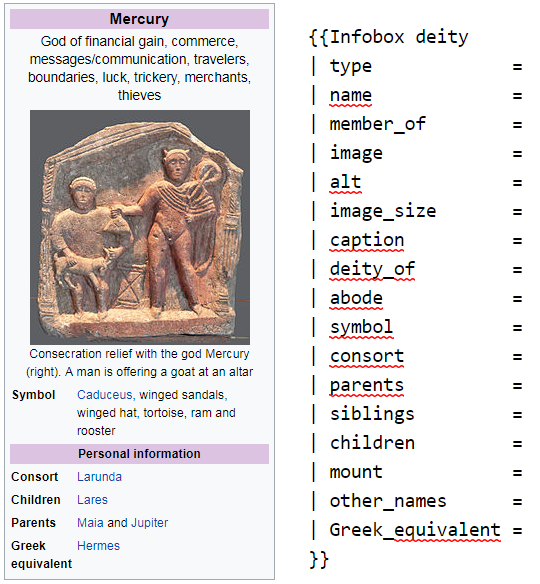
\includegraphics[width=0.8\linewidth]{mercury-infobox}
  \caption{Example Infobox of the page related to the god Mercury with the default properties for infoboxes about deities.}
  \label{fig:mercury-infobox}
\end{figure}



\subsubsection{\hspace*{3pt} Categories}

Every Wikipedia article should have at least one category. Categories are collections that identify topics in the encyclopedia. 

The category structure is not a tree. Therefore some categories have multiple supercategories, and one article can belong to several categories. In the same way as links, categories show a semantic structure between Wikipedia articles. 

It should be noted that although the structure of the Wikipedia category forms a taxonomy, it is not represented by a simple tree of categories and subcategories but, in fact, by a complex graph. This graph allows multiple categorizations of topics simultaneously, which means that one category may have multiple parents. The category "Semantics" is a good example of this complex structure since it is a subcategory of ``Grammar",  ``Linguistics", ``Concepts in logic", ``Semiotics", ``Philosophy of language" and others (see \ref{fig:semantics-category}).


\begin{figure}[H]
\centering
  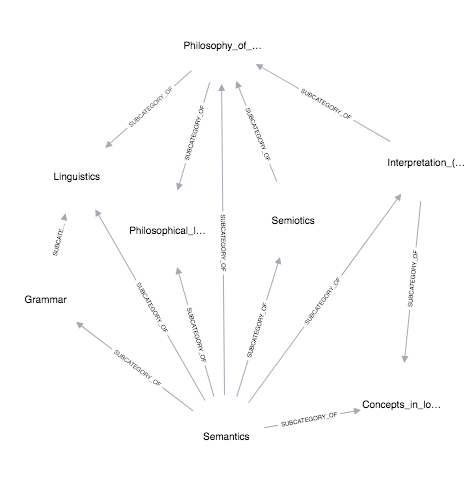
\includegraphics[width=0.8\linewidth]{graph-semantics}
  \caption{Example of an induced graph showing the supercategories of ``Semantics" in the Wikipedia Category Graph}
  \label{fig:semantics-category}
\end{figure}

Although not a semantic basis, Wikipedia has a set of characteristics, such as the definition of a large number of articles and organization of articles in categories, which makes an essential semantic resource.

A simple example, but one that illustrates well the complexity of the relationships between Wikipedia categories is the Apple concept (the fruit) , which is directly linked to four categories: ``Apples", ``Malus", ``Fruits originating in Asia," and ``Plants described in 1768". Each of these categories has been added and cured by people who are part of the Wikipedia community. In addition to the explicit knowledge in the directly attributed categories, a vast implicit knowledge can be inferred by the relations between them, both generically and in a specific way. If we take as starting point the category Apples, from the analysis of their links to the top of the classification, we perceive a more general case: Apples $\rightarrow$  Edible Fruits $\rightarrow$ Edible Plants $\rightarrow$ Food $\rightarrow$ Food and Drink $\rightarrow$ Health.
To illustrate a more specific case, let us take the Malus category as the origin and analyze one of the possible paths to the top: Malus $\rightarrow$ Maleae $\rightarrow$ Prunoideae $\rightarrow$ Rosaceae $\rightarrow$ Rosales $\rightarrow$ Rosids $\rightarrow$ Core Eudicots $\rightarrow$ Eudicots $\rightarrow$ Angiosperms $\rightarrow$ Plants $\rightarrow$ Eukaryota $\rightarrow$ Organisms $\rightarrow$ Life.
These are just examples of small fragments in Wikipedia's categorization structure for the Apple concept. The complete structure involves 33 different categories and 42 different relations between them (See figure \ref{fig:semantics-category-apple}).


\begin{figure}[H]
\centering
  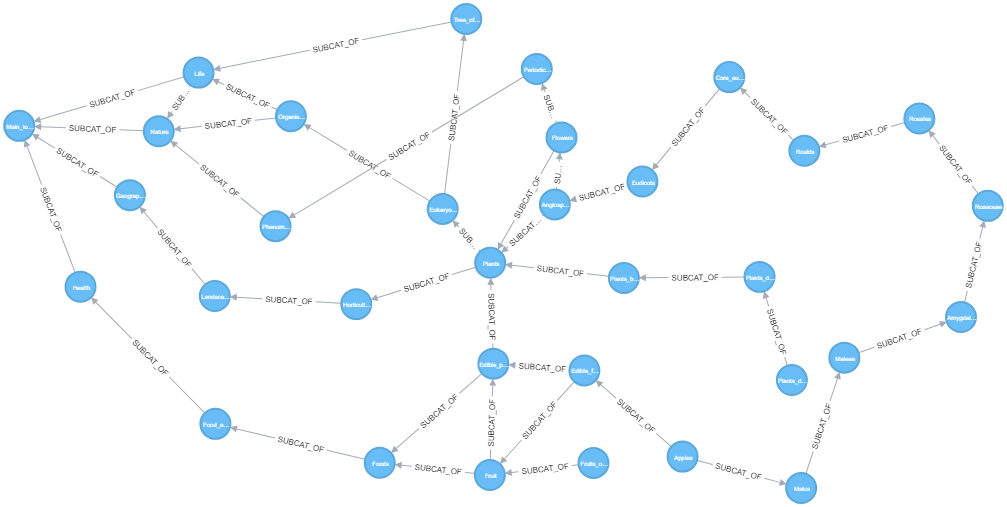
\includegraphics[width=0.8\linewidth]{graph}
  \caption{Example of an induced graph showing the categories and relationships for the Entity Apple towards Main topics}
  \label{fig:semantics-category-apple}
\end{figure}


\subsection{\hspace*{3pt} DBpedia}

As described directly on the DBpedia about page\footnote{url{https://wiki.dbpedia.org/about}} DBpedia is 

\begin{displayquote}
\say{
\textit{
a crowd-sourced community effort to extract structured content from the information created in various Wikimedia projects. This structured information resembles an open knowledge graph (OKG) which is available for everyone on the Web. A knowledge graph is a particular kind of database which stores knowledge in a machine-readable form and provides a means for information to be collected, organized, shared, searched and utilized.}
}
\end{displayquote}


The DBpedia dataset has many advantages compared to the raw data from Wikipedia. Besides the more convenient access to the underlying Wikipedia data sources, it also provides a higher data quality. The higher quality is because the extraction framework embeds multiple steps commonly found in data mining applications, such as duplicate removal in the form of mapping redundant infobox properties to the same DBpedia property.
Therefore, the present work is focussed on using DBpedia for the entity named recognition and Linking, as well as for traversing entities' categories.


\subsubsection{\hspace*{3pt} SPARQL}

\gls{sparql} is a query language capable of retrieving and manipulating data stored in the \gls{rdf} format that is the basis of the OWL language. \gls{rdf} is a labeled and directed data format used to represent information on the Web \cite{prud2008sparql}. 

In the context of this research, our approach exploits a small part of what the SPARQL language can provide. We  navigate in the DBpedia hierarchy to retrieve broader semantic relations between the entities and its categories. 

    \chapter{\hspace*{3pt} Methods}
\label{chapter:methodology}

%Automatic text classification consists of automatically assigning a predefined label to textual documents. The use of text classification can be observed in (i) organization through routing, filtering and metadata assignments; (ii) analysis, through the statistics of the labels assigned to the documents or through descriptive and predictive analyzes; and (iii) knowledge extraction, through a set of rules or values that summarize the patterns present in the collection of documents. 
%Moreover, information retrieval engines which correspond to many of the use of the Internet for locating information and gaining knowledge, make use of text classification algorithms to rank the most relevant documents according to a user's query ~\cite{Manning:2008}.

%To perform automatic text classification, expert systems or machine learning algorithms may be used. In the first case, one or more domain experts create a set of conditional rules based on the presence or frequency of a set of words or sentences that define the class of a document. However, manually generated rules are complicated to create or update for different applications or domains and are dependent on the presence and effort of domain experts or knowledge engineers~\cite{Manning:2008}. 

%For that reason, automatic text classification is one of the most studied and used areas to accomplish the tasks mentioned above. 

This chapter presents in detail the steps of our approach for the extraction and representation of document features based on the Wikipedia category graph. The implementation details for filtering and building the graph are also presented.


%Finally, we perform a graph-theoretic analysis of the \gls{wcg} to describe the topology of the graph and to evaluate whether graph-based techniques for semantic analysis and information retrieval can be applied to it.


\section{\hspace*{3pt} Approach} \label{sec:approach}

The rich structure of the Wikipedia Category Graph has contributed to make it a large and meaningful semantic taxonomy. That said, our main goal is to take advantage of this body of knowledge to automatically categorize any text-based content on the Web following the collective knowledge of Wikipedia contributors. A processing chain to generate a generic categorization was developed based on three steps: 

\begin{enumerate}
\item Text annotation;
\item Categories extraction; and
\item Document Representation.

\end{enumerate}
As the basis for our approach, we consider the relationships of Wikipedia Categories as a directed graph. Let $G$=($V$, $E$) be a graph, where $V$ is the set of nodes representing Wikipedia categories, and $E$ is the set of edges representing the relationships between two categories.

To make it simple to understand, let us illustrate the steps.

\subsection{\hspace*{3pt} Text Annotation} 
\label{sec:text-annotation}
When dealing with the Web of Documents, we are primarily working with unstructured data, which, in turn, hinders data manipulation and the identification of atomic elements in texts. To alleviate this problem, \gls{ie} methods, such as \gls{ner} are employed. These methods automatically extract structured information from unstructured data and make it possible to link them to external knowledge bases. 

In the context of this thesis, we chose DBpedia as our Knowledge Base because it covers many domains (Science, Arts, Politics, History, Geography, Health and Nature, among others). Another reason is its constant evolution. Since the knowledge in DBPedia is extracted from Wikipedia,  the Knowledge Base is also continuously updated by the contributors. DBpedia is also available in different languages and can be accessed either by an endpoint\footnote{\url{http://dbpedia.org/sparql/}} or being installed in a local machine, making it faster to process a vast amount of data.

Based on a comparison made by Gangemi\cite{gangemi2013comparison} we decided to use the DBpedia Spotlight  tool\footnote{\url{http://dbpedia-spotlight.github.io/demo/}} for entity extraction and linking to DBpedia. Even though there are some options (such as AIDA\footnote{\url{https://github.com/codepie/aida}} or Alchemy\footnote{\url{https://www.ibm.com/watson/alchemy-api.html}}) that outperform Spotlight for the task of \gls{ner}, they fail to meet some criteria. For instance, AIDA is directly linked to YAGO and Alchemy is a paid API with limited access.  


DBpedia Spotlight is a system for automatically annotating text documents with DBpedia URIs. It contains Wikipedia's encyclopedic knowledge of about 3.5 million resources, where nearly half of the knowledge base is classified according to the following ontologies: people, organizations or places\cite{Mendes:2011}. 

The DBpedia Spotlight was used to extract and enrich entities found in the Web resources.

For instance, after processing the following Web resource using an \gls{ie} tool: ``I agree with Barack Obama that the whole episode should be investigated.", the entity  ``Barack Obama" is annotated, classified as ``person" and linked to the DBpedia resource: \\ 
 <http://dbpedia.org/resource/Barack\_Obama>, where structured information about the entity is available, as exemplified in figure \ref{fig:dbpedia-annotation}.
 
 
\begin{figure}[H]
  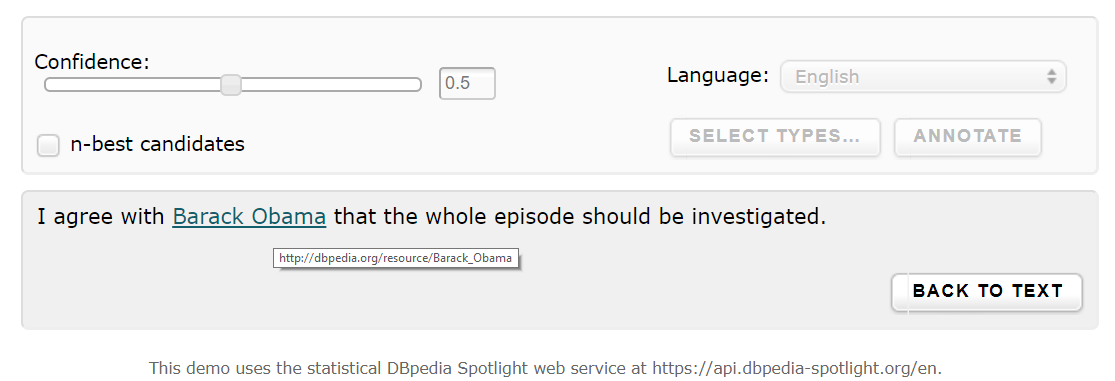
\includegraphics[width=\linewidth]{dbpedia_annotation}
  \caption{Example of text annotation by Named Entity Recognition using DBpedia SPotlight}
  \label{fig:dbpedia-annotation}
\end{figure}


 
Note that this method is language-independent as long as we have a repository of entities (such as DBpedia) and a proper annotation tool (such as DBpedia Spotlight, Apache Stanbol\footnote{\url{https://stanbol.apache.org}} or AIDA). However, the set of entities that can be identified by the annotation process is limited to the number of known entities in the dataset; in this case, DBpedia datasets in English, Dutch, French, German, Italian, Portuguese, Russian, Spanish, Hungarian and Turkish.

\subsection{\hspace*{3pt}  Categories Extraction}
\label{sec:categories-extraction}
Given the entities found in the previous step as a starting point, the categories extraction step begins by traversing the entity relationships to find a more general representation of the entity, i.e., their categories. All categories associated to the entities identified in the source of information are extracted. 

For instance, for each extracted and enriched entity in a Web resource, we explore the relationships through the predicate [dcterms:subject], which by definition represents the categories of an entity. In that sense, to retrieve the topics, we use SPARQL query language for \gls{rdf} over the DBpedia SPARQL, where we navigate up in the DBpedia hierarchy to retrieve broader semantic relations between the entities and its topics. 

Note that an entity/concept can be found in different levels of the hierarchical categories of DBpedia. Hence this approach would lead us to retrieve topics in different category levels. 

\subsection{\hspace*{3pt} Representation of Document}
\label{sec:doc-representation}

The goal of this step is to figure out how the resource page being tagged is related to a more generic subset of Wikipedia categories. 

In the top of Wikipedia categorization stricture, under the ``Contents" category there is the category ``Main topic classifications"\footnote{\url{https://en.wikipedia.org/wiki/Category:Main_topic_classifications}} that has 19 subcategories representing different fields of study, hence we used the subcategories of ``Main topic classifications" as a subset of the Wikipedia Categories for the context of this thesis. 

The algorithm \ref{alg:fingerprint-generation} begins with the categories assigned to entities recognized in the text and generates a categorization based on the frequency of assignments with the top-level categories in Wikipedia, the so-called Main topic classifications.

To define the problem of automatically assigning categories to resources let $D = \{d_1,d_2,d_3,\ldots\,d_n\}$ be a finite set of documents and $C = \{c_1,c_2,c_3,\ldots\,c_n\}$ a finite set of predefined categories.
The problem is finding a function $f: D \times C \mapsto \mathbb{R}$ that assigns a score $s$ for each pair 
$\{d_i, c_i\} \in  D \times C $, where the membership value of  $s$ specifies the degree of relevance of the category $c_i$ to the document $d_j$.


Our approach consists of navigating in the Category Graph from each category extracted in the previous step towards the top of the graph by all the shortest paths between the category and the main topics.  

The Category Graph is not a perfect hierarchical structure. It is noisy, contains cycles and many of the paths from a category to the main topic classifications do not make sense. One of the main reasons for that is that users who add categories to Wikipedia pages often assign them to small grained categories in the graph. Most of the time they don't fully understand the internal structure of the graph and don't fallow the guidelines when choosing particular categories. The category graph as well as the content of the articles can be changed over time, also changing the original intent of the author and the meaning of the category assignments.

Since the Category Graph is being used as a taxonomy, we decided to use the shortest path to alleviate this problem. We based our decision on the results of previous works. Kittur\cite{knuth:84} tested many heuristics and the shortest paths between categories showed to be the best approach. 

Strube and Ponzetto\cite{strube2006wikirelate} developed a system named WikiRelate!. They used data from Wordnet, Wikipedia, and Google for computing degrees of semantic similarity and reported that Wikipedia outperforms Wordnet.  They used different measures for computing semantic relatedness and showed good results with the one based on shortest paths.

Each time the source category reaches one of the top-level categories by the shortest paths, we update the influence of this top category in the composition of the resource classification.

Based on the influence of each main topic category in the resource being tagged, we generate a representation of the document based on the calculated categorization as a multidimensional vector.

The \gls{vsm} is a simple, traditional and practical model that makes it possible to represent documents as vectors and perform any algebraic operation to compare them ~\cite{salton1988term}.

In this method, the documents of a collection $D$ are represented in the VSM as points in a multidimensional Euclidean space, where each dimension corresponds to a distinct term in that collection. The set $T$ of distinct terms of collection $D$, called vocabulary collection of $D$, is obtained in a process called lexical analysis.


This type of representation is widely used in Information Retrieval, both in tasks of textual retrieval and ordering of documents by relevance (ranking), as well as in document classification tasks. The use of vector representation makes possible the use of any algebraic operation applicable to this type of structure, making it possible to compare the similarity between two documents, as explained by Salton\cite{Salton:1975}.


Each term of the set $T$ can be composed of only one word (unigrams), several words (bigrams, trigrams or n-grams) or sentences, and has an associated weight to determine its degree of importance ~\cite{salton1988term}.

Given a document $d_i \in D$, this document is formally represented in the \gls{vsm} as follows:

$d={w_{i1},w_{i2},w_{i3},\ldots,w_{i|T|}}$,

where $T$ is the vocabulary set of the collection $D$ and $w_{ij} (1 \le j \le |T|)$ is the weight of the term $t_j$ in the document $d_i$, such that $w_{ij} = 0$ if the term $t_j$ does not occur in the document $d_i$.

As a formal definition of our approach, lets denote $I$ as the set of categories related to a web resource $d$, found in the category extraction step. $C$ is the set of all Categories in Wikipedia and $M$ is the set of categories that represent the main topics. $G = (V,E)$, where $I \subset V ; C \subset V ; M \subset V$; and $M \subset C$.  The parameter  $l$ is defined to indicate the broadest $l$ levels to be considered in the set of $M$. If $t$ is 1, only the main topics previously defined are considered; if $t$ is 2, any category 1 edge away in the graph is also considered as a main topic. The weight $w$ is defined to make it possible to assign different weights for 

Note that a path is a sequence of graph vertices visited from a given category $c \in C$ to a main topic $m \in M$.  

\begin{algorithm}
\caption{Vector Generation}\label{alg:fingerprint}
\label{alg:fingerprint-generation}
\begin{algorithmic}[1]
\Procedure{GenerateVector}{$G,M, I, t, w$}
\State $E\gets$ a map from a list of categories $ m \in M$
\For {$i \in I$}
\State $S\gets$ the set of shortest paths between $i$ and any category in $M$
\For {$s \in S$}
\State $B\gets$ the set of last $t$ vertices in path $s$
\For {$b \in B$}
\State $E[b]\gets E[b] + w$
\EndFor
\EndFor
\EndFor
\State \textbf{return} $E$
\EndProcedure
\end{algorithmic}
\end{algorithm}


In all experiments described in this paper, only the subcategories of Main\_top\_classifications were considered in the set of  $M$ (i.e. Arts, Culture,Games,Geography,Health, History, Humanities, Industry, Law, Life, Mathematics, Matter, Nature, Philosophy, People, Reference works, Religion, Science and technology and Society) it means that we fixed the parameter $t$ with a value of $1$. In effect, as a result of this method we have a 19-sized vector, representing the content of a given text-based resource.

\section{\hspace*{3pt} A running example}

To illustrate how the method works in a real application scenario, we present a step-by-step example in a text extracted from the Internet.

The text is an excerpt from the article entitled ``Market Totalitarianism in North Korea", taken from The New York Times\footnote{\url{https://www.nytimes.com/}} of May 3, 2017: \

\textit{"(...) Post-Communist, postindustrial, kleptocratic dynastic regime of North Korea may become the crown jewel of the new axis-of-tyranny ideology (...)"}\footnote{\url{https://nyti.ms/2py3z4r}} \

\subsection{\hspace*{3pt} Processing step 1 - Text Annotation} 

As mentioned in section \ref{sec:text-annotation}, our approach starts by extracting structured data from unstructured text by recognizing the named entities present in the text-based resource and linking them to DBpedia. 

After using DBpedia Spotlight to extract the concept from the excert, we obtain the entities linked to DBpedia as shown in table \ref{tab:example-entities}.

% Please add the following required packages to your document preamble:
% \usepackage{booktabs}
\begin{table}[H]
\centering
\caption{Entities extracted from the text and their respective links to DBpedia concepts.}
\label{tab:example-entities}
\begin{tabular}{@{}ll@{}}
\toprule
Entity in Text & Link to Dbpedia                                  \\ \midrule
postindustrial & http://dbpedia.org/resource/Post-industrial\_society \\
kleptocratic   & http://dbpedia.org/resource/Kleptocracy              \\
dynastic       & http://dbpedia.org/resource/Dynasty                  \\
North Korea    & http://dbpedia.org/resource/North\_Korea             \\
tyranny        & http://dbpedia.org/resource/Tyrant                   \\ \bottomrule
\end{tabular}
\end{table}


\subsection{\hspace*{3pt} Processing step 2 - Categories Extraction}

As described in the section \ref {sec:categories-extraction}, the second step consists of extracting all categories related to all entities found in the text.
Using a \gls{sparql} query that retrieves all categories (dc:subject predicate) associated with the entities listed in table \ref{tab:categorylinks} we obtain the categories listed in table \ref{tab:entities-categories}.


\begin{table}[H]
\centering
\caption{List of all entities extracted from the example test and the categories associated to them}
\label{tab:entities-categories}
\begin{tabular}{@{}ll@{}}
\toprule
\textbf{Entity}         & \textbf{Categories}                                                                                                                                                                                                                                                                                                                                                                                                        \\ \midrule
Post-industrial society & \begin{tabular}[c]{@{}l@{}}Postindustrial society \\ Information economics\\ Postmodernism\\ Social philosophy\\ Technology in society\\ Theories of history\end{tabular}                                                                                                                                                                                                                                                  \\
\rowcolor[HTML]{EFEFEF} 
Kleptocracy             & \begin{tabular}[c]{@{}l@{}}Forms of government\\ Political corruption\\ Political terminology\end{tabular}                                                                                                                                                                                                                                                                                                                 \\
Dynasty                 & \begin{tabular}[c]{@{}l@{}}Royal families\\ History-related lists\\ Monarchy\end{tabular}                                                                                                                                                                                                                                                                                                                                  \\
\rowcolor[HTML]{EFEFEF} 
North Korea             & \begin{tabular}[c]{@{}l@{}}1948 establishments in North Korea\\ Communist states\\ Countries in Asia\\ East Asian countries\\ Korea\\ Korean-speaking countries and territories\\ Member states of the United Nations\\ Military dictatorships\\ North Korea\\ Northeast Asian countries\\ One-party states\\ Republics\\ Socialist states\\ States and territories established in 1948\\ Totalitarian states\end{tabular} \\
tyranny                 & \begin{tabular}[c]{@{}l@{}}Ancient Greek government\\ Ancient Greek titles\\ Ancient Roman government\\ Positions of authority\\ Ancient Greek tyrants\end{tabular}                                                                                                                                                                                                                                                        \\ \bottomrule
\end{tabular}
\end{table}


\subsection{\hspace*{3pt} Processing step 3 - Document Representation}

In this last step, as detailed in section \ref{sec:doc-representation}, we generate a vector that represents the document based on the count of shortest paths between all categories associated with entities extracted from the text-based resource and a set of more generic categories in the \gls{wcg}. The induced graph for this example contains 143 distinct categories and 256 relationships and can be seen in figure \ref{fig:graph-example}.

 
\begin{figure}[H]
  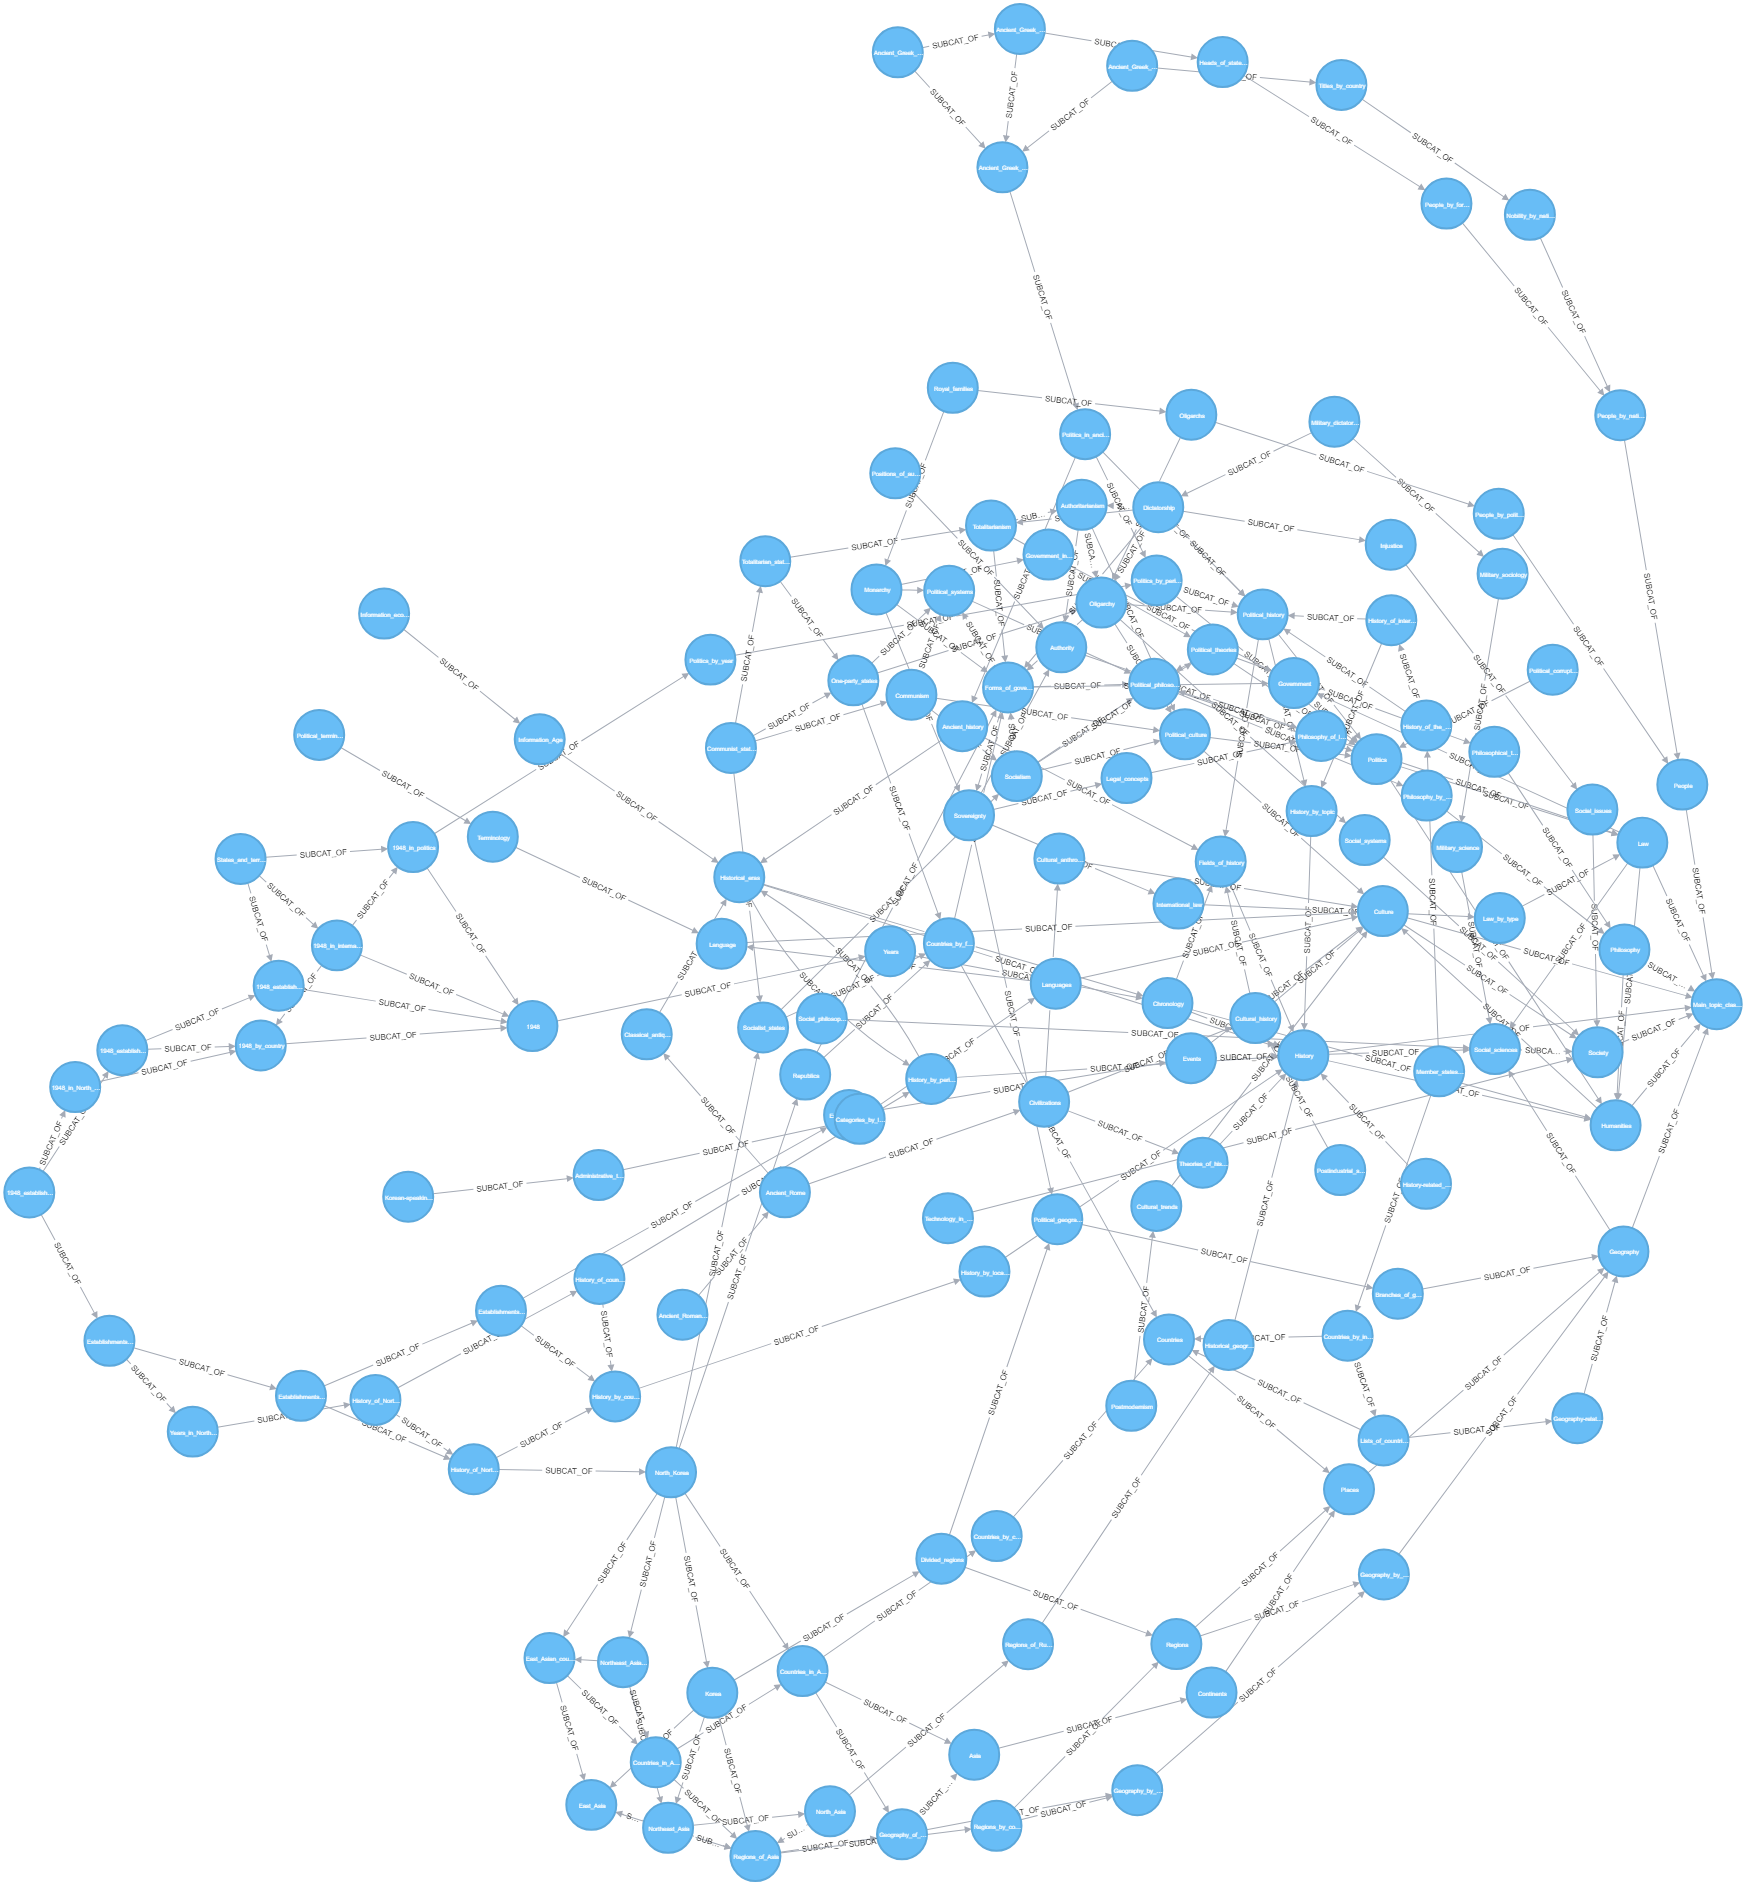
\includegraphics[width=\linewidth]{graph-example}
  \caption{An induced graph containing all shortest paths from the categories found and described in table \ref{tab:entities-categories} and ``Main topic classifications" (on the right of the graph)}
  \label{fig:graph-example}
\end{figure}


The vector generated for this examples is shown in table \ref{tab:vector}. Note that this is the representation of the document based only on a small excerpt. 
We can infer that this document is strongly related to History, Humanities, Law, and Culture, and also has some weaker relatedness to Society, Geography, Philosophy, and People. Bellow we present one random example of a path for each top-level category that contributed to the document representation.


\begin{itemize}

\item Theories of history $\rightarrow$ \textbf{History} 

\item Political corruption $\rightarrow$ Politics $\rightarrow$ \textbf{Humanities}

\item Political corruption $\rightarrow$ Politics $\rightarrow$ \textbf{Law} 


\item Totalitarian states $\rightarrow$ Totalitarianism $\rightarrow$ Authoritarianism $\rightarrow$ Political culture $\rightarrow$ \textbf{Culture}


\item Military dictatorships $\rightarrow$ Dictatorship $\rightarrow$ Oligarchy $\rightarrow$ Social systems $\rightarrow$ \textbf{Society} 


\item 
Korea $\rightarrow$ Divided regions $\rightarrow$ Political geography $\rightarrow$ Branches of geography $\rightarrow$ \textbf{Geography}


\item Forms of government $\rightarrow$ Political philosophy $\rightarrow$ Philosophy by topic $\rightarrow$ \textbf{Philosophy}

\item Royal families $\rightarrow$ Oligarchs $\rightarrow$ People by political orientation $\rightarrow$ \textbf{People} 


\end{itemize}


% Please add the following required packages to your document preamble:
% \usepackage{booktabs}
\begin{table}[H]
\centering
\caption{The 19-sized vector representing the document based on the top-level categories of \gls{wcg}}
\label{tab:vector}
\begin{tabular}{@{}ll@{}}
\toprule
Top-level Categories     & Shortest paths \\ \midrule
History                  & 29             \\
Humanities               & 23             \\
Law                      & 21             \\
Culture                  & 17             \\
Society                  & 9              \\
Geography                & 8              \\
Philosophy               & 5              \\
People                   & 3              \\
Religion                 & 0              \\
Matter                   & 0              \\
Life                     & 0              \\
Industry                 & 0              \\
Games                    & 0              \\
Arts                     & 0              \\
Science\_and\_technology & 0              \\
Health                   & 0              \\
Reference\_works         & 0              \\
Nature                   & 0              \\
Mathematics              & 0              \\ \bottomrule
\end{tabular}
\end{table}






\section{\hspace*{3pt}Implementation Details}
In the scope of this thesis, finding the paths between entities and a set of top categories requires that the structure of Wikipedia Category is represented so that computer programs can navigate on it. 

Therefore, we needed a way of representing the available information about the Wikipedia structure as a graph. The Wikipedia Category Graph consists of Wikipedia pages with the “Category:” prefix such as “Category:Law”. The graph is extracted by finding links between category pages. In other words, a category page is liked to another category page that is broader in scope.

To perform this task, we obtained a dump of the files enwiki-latest-page.sql, enwiki-latest-category.sql and enwiki-latest-categorylinks.sql, in October 2016 \footnote{\url{https://dumps.wikimedia.org/enwiki/20161020\/}}.

These files consist the structure of Wikipedia represented in a MySQL relational database.

The file enwiki-latest-categorylinks.sql.gz contains the information needed to extract the categories-categories and categories-articles relations. The information is represented in the file as INSERT statements where all entries are on the form: \\
\textit{
(cl\_from,cl\_to,cl\_sortkey,cl\_timestamp,cl\_sortkey\_prefix,cl\_collation,cl\_type). }



\begin{table}[H]
\begin{adjustbox}{width=1\textwidth}
\begin{tabular}{@{}ll@{}}
\toprule
Field               & Description                                                                                                   \\ \midrule
cl\_from            & Stores the page.page\_id of the article where the link was placed                                             \\
cl\_to              & Stores the name (excluding namespace prefix) of the desired category. Spaces are replaced by underscores (\_) \\
cl\_sortkey         & Stores the title by which the page should be sorted in a category list.                                       \\
cl\_timestamp       & Stores the time at which that link was last updated in the table.                                             \\
cl\_sortkey\_prefix & either an empty string if a page is using the default sortkey or a human readable version of cl\_sortkey.     \\
cl\_collation       & What collation is in use.                                                                                    \\
cl\_type            & What type of article is this (file, subcat (subcategory) or page (normal page)).                              \\ \bottomrule
\end{tabular}
\end{adjustbox}
\caption{Description of fields in INSERT statements for the table categorylinks.}
\label{tab:categorylinks}
\end{table}

<EXAMPLE OF INSERT STATEMENTS HERE>

Considering the goal of this process is to represent the underlying Wikipedia category structure as a graph, we chose to use Neo4J \footnote {\url{https://neo4j.com/}}, a graph-based database that provides a free version and proper documentation, as well as an active community. 

Even though only the category graph is needed, it was necessary to extract the page file as well, since the identifier of the categories refers not to the categories themselves, but to the page about the categories. For this step, a parser was developed in python. First, the file containing all the pages of Wikipedia is scanned and, through a regular expression, the data is filtered.

The output is a CSV file with three fields: page identifier, page title, and namespace. Namespaces are a Wikipedia internal classification system to identify what a page refers to, such as an article, a category, user page, or other classifications. Articles are identified with namespace 0 and categories with namespace 14, for example.
The second step is to go through the file that corresponds to the categories of Wikipedia. The output of this step is a CSV file with two properties: page identifier and category title. From this file, it is possible to link the categories and the corresponding pages. The third and final step of this step is the extraction of links between categories. The data is extracted from the file of the enwiki-latest-categorylinks.sql file, and the output is a csv file with two properties: page identifier for the source category and page identifier for the destination category.

Administrative categories are used for Wikipedia internal organization and mantaining. They were ignored during processing and are not in the final files. Examples of these categories include, but are not limited to, categories that begin with \textit{Articles\_needing\_} and \textit{WikiProject\_}, named hidden categories.


These categories provide a tool for grouping pages with features in common so that publishers can quickly identify where improvements are needed. Although these categories are essential for the maintenance and administration of the encyclopedia, they are not relevant to end users and were removed in the context of the work for two reasons: 1) They add complexity to the structure of the graph 2) They do not semantically describe articles associated to them and therefore do not add relevant information to the paths.


The ideal paths between a set of categories have no hidden categories. Thus, the hidden categories must be removed in such a way that the information is not lost because a hidden category can be a subcategory of a visible category or they can have visible categories as their subcategories

<EXAMPLE OF HIDDEN CATEGORIES REMOVAL HERE>

After processing the Wikipedia dump files, it is possible to generate the complete graph of categories. First, we import all the pages referring to categories in the Neo4J, and then the relations between them are imported. The generated graph has only a $Category$ concept with the $categoryName$ and $categoryID$ properties and a $SUBCATEGORY\_OF$ relationship type, with no properties.

The example below illustrates how information retrieval works in a Neo4J graph.

The example returns all nodes of type $Category$  that are connected to another node of type $Category$ that has the property $CategoryName$ with the value equals to Carnivores for the $SUBCATEGORY_OF$ property. In this case, all subcategories of Carnivores are retrieved.

\begin{verbatim}
MATCH (a: Category) - [r: SUBCATEGORY_OF] ->
(b: Category {categoryName: ""}) RETURN a
\end{verbatim}





  
 	\chapter{\hspace*{3pt} Experiments and Results}
\label{chapter:experiments}

Esse capítulo descreve os experimentos computacionais e os testes 

\section{\hspace*{3pt} Proof of Concept - Q\&A Communities}
\label{section:proof-of-concept}

The first evaluation of our approach is a proof of concept aiming to analyze the classification based on our method in posts of  Q\&A (Question and Answers) communities. 

Q\&A (Question and Answers) have emerged in the past few years as Web 2.0 becomes popular. They provide a place for users to ask specific questions and receive direct answers. 
The users exchange and share their knowledge explicitly by asking or answering questions in a set of predefined topics and categories. 

The volume of questions answered on Q\&A site so far exceeds the number of questions answered by library reference services \cite{Shah:2010} . As a result,  question and answer archives are numerous knowledge repositories \cite{Andrzejewski:2009}.


In this context, Stack Exchange\footnote{\url{https://stackexchange.com/}}
is a network of 133 Q\&A communities on topics in varied fields, each community covering a specific theme, where questions, answers, and users are subject to a reputation award process.

For our evaluation, we decided to use Stack Exchange because it covers a wide variety of topics and also because they make data available publicly in a structured way. 

We relied on an anonymized dump of all user-contributed content on the Stack Exchange network, extracted on August 31st 2017\footnote{\url{https://archive.org/details/stackexchange}}. Each site is formatted as a separate archive consisting of XML files from Posts, Users, Votes, Comments, PostHistory and PostLinks. We used the Posts files as the basis for this experiment. As per the description of the dataset, the property postTypeId denotes if the given row in the file is a question or an answer. 

We selected ten representative communities on stack exchange to perform this evaluation: 

\begin{description}
\item [Math:] A question and answer community for professional mathematicians.
\item [Chemistry:] A question and answer community for scientists, academics, teachers, and students of chemistry.
\item [Biology:] A question and answer community for biology researchers, academics, and students.
\item [Music:]  A question and answer community for musicians, students, and enthusiasts. 
\item [Christianity:] A Question and answer community for committed Christians, experts in Christianity other people interested in learning more about the topic.
\item [Philosophy:]  A question and answer community for those interested in the study of philosophy.
\item [History:] A question and answer community for historians and fans of history buffs.
\item [Law:] A question and answer community for legal professionals, students, and others with experience or interest in law.

\item [Astronomy:] A question and answer community for astronomers and astrophysicists. 

\item[Sports:] A question and answer community for participants, hobbyists, and fans of all sports and forms of competitive physical activity.
\end{description}


Table \ref{tab:stackdist} displays the number of posts by type found in the datasets. Note that the column unknown is relative to post that were identified neither as a question nor as an answer. 


\begin{table}[H]
\centering
\caption{Distribution of post type in the stack exchange datasets}
\label{tab:stackdist}
\begin{tabular}{@{}llll@{}}
\toprule
Community                            & Questions & Answers & Unknown \\ \midrule
mathoverflow.net.count               & 84657     & 124683  & 1029    \\
chemistry.stackexchange.com    & 23074     & 26997   & 646     \\
biology.stackexchange.com      & 15934     & 19009   & 1068    \\
music.stackexchange.com        & 11101     & 29980   & 770     \\
christianity.stackexchange.com & 9267      & 22043   & 1446    \\
philosophy.stackexchange.com   & 8619      & 20474   & 299     \\
history.stackexchange.com      & 7339      & 14657   & 681     \\
law.stackexchange.com          & 6337      & 7815    & 472     \\
astronomy.stackexchange.com    & 5019      & 7383    & 437     \\
sports.stackexchange.com       & 3711      & 5830    & 656     \\ \bottomrule
\end{tabular}%

\end{table}


For each row in the Post.xml file of each one of these communities, we executed the three steps of the chain described in Section \ref{sec:approach}. We first extracted the entities present in each post, than we linked the entities with their categories in DBPedia and finally we traversed the \gls{wcg} by the shortest paths to the top-level categories. 


 \begin{figure}[H]
    \centering
    \begin{subfigure}{0.5\textwidth}
    \centering
        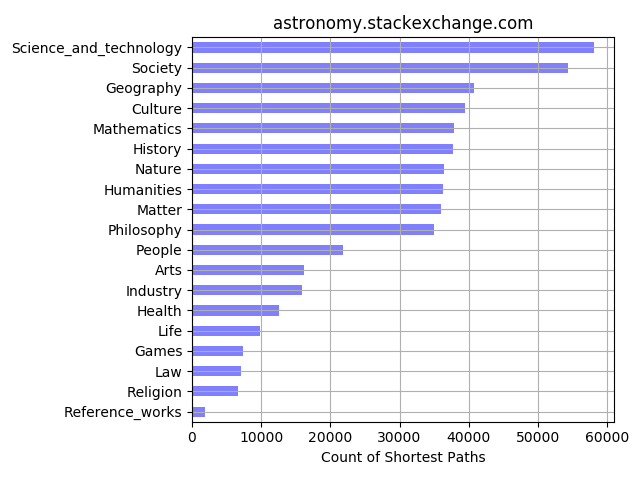
\includegraphics[width=1\linewidth]{imgs/path-counts/astronomy_stackexchange_com}
        \caption{Paths count for Astronomy}
        \label{fig:path-count-astronomy}
    \end{subfigure}%
    \begin{subfigure}{0.5\textwidth}
    \centering
        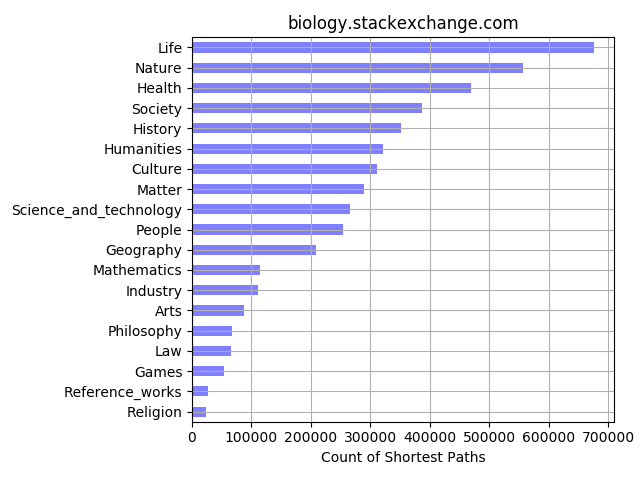
\includegraphics[width=1\linewidth]{imgs/path-counts/biology_stackexchange_com}
        \caption{Paths count for Biology}
        \label{fig:path-count-biology}
    \end{subfigure}
 
     \begin{subfigure}{0.5\textwidth}
    \centering
        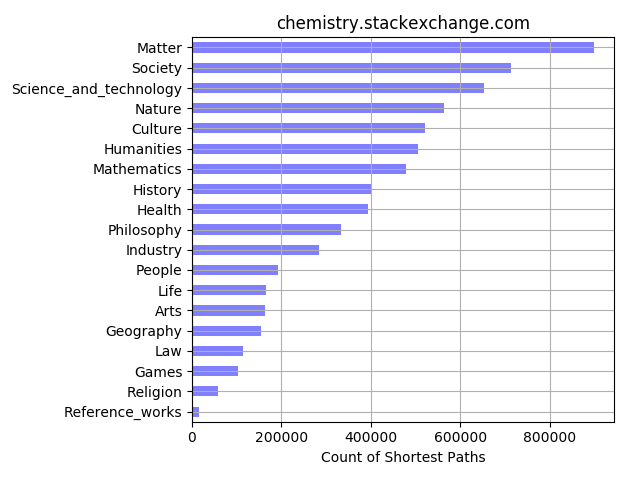
\includegraphics[width=1\linewidth]{imgs/path-counts/chemistry_stackexchange_com}
        \caption{Paths count for Chemistry}
        \label{fig:path-count-chemistry}
    \end{subfigure}%
    \begin{subfigure}{0.5\textwidth}
    \centering
        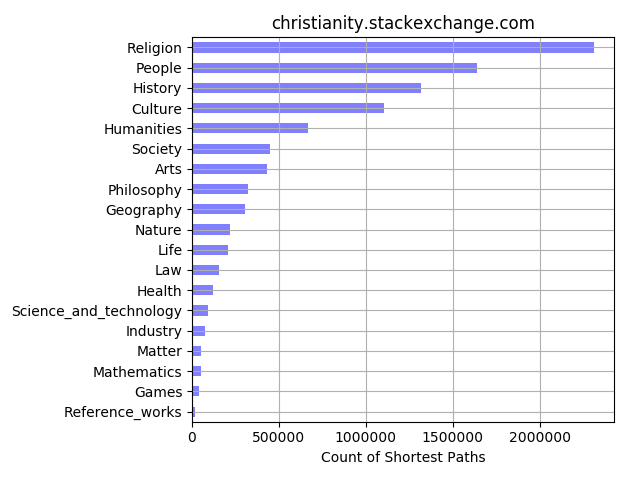
\includegraphics[width=1\linewidth]{imgs/path-counts/christianity_stackexchange_com}
        \caption{Paths count for Christianity}
        \label{fig:path-count-christianity}
    \end{subfigure}

        
     \begin{subfigure}{0.5\textwidth}
    \centering
        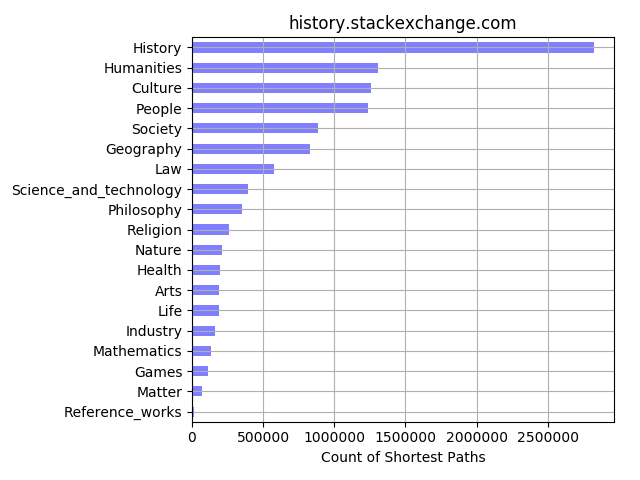
\includegraphics[width=1\linewidth]{imgs/path-counts/history_stackexchange_com}
        \caption{Paths count for History}
        \label{fig:path-count-history}
    \end{subfigure}%
    \begin{subfigure}{0.5\textwidth}
    \centering
        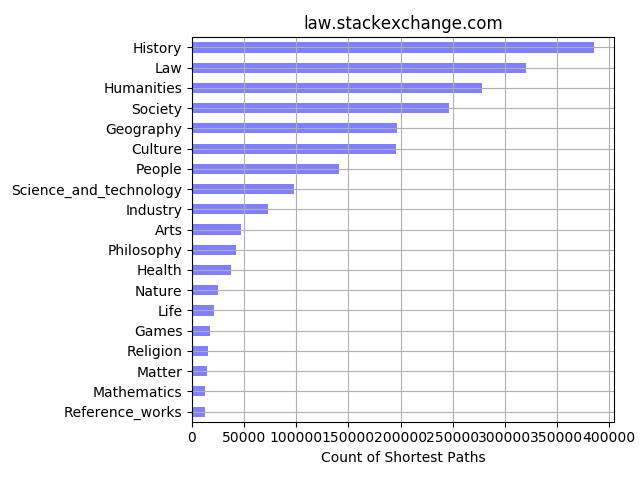
\includegraphics[width=1\linewidth]{imgs/path-counts/law_stackexchange_com}
        \caption{Paths count for Law}
        \label{fig:path-count-law}
    \end{subfigure} 

    \end{figure}
    
 \begin{figure}[H]
 \ContinuedFloat
    \centering
    \begin{subfigure}{0.5\textwidth}
    \centering
        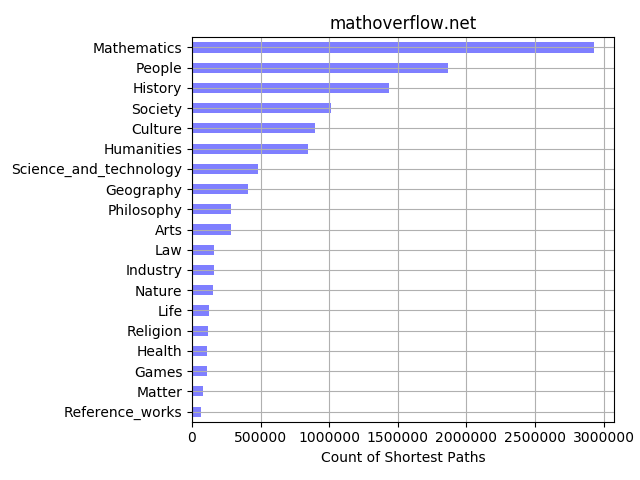
\includegraphics[width=1\linewidth]{imgs/path-counts/mathoverflow_net}
        \caption{Paths count for Math}
        \label{fig:path-count-math}
    \end{subfigure}%
    \begin{subfigure}{0.5\textwidth}
    \centering
        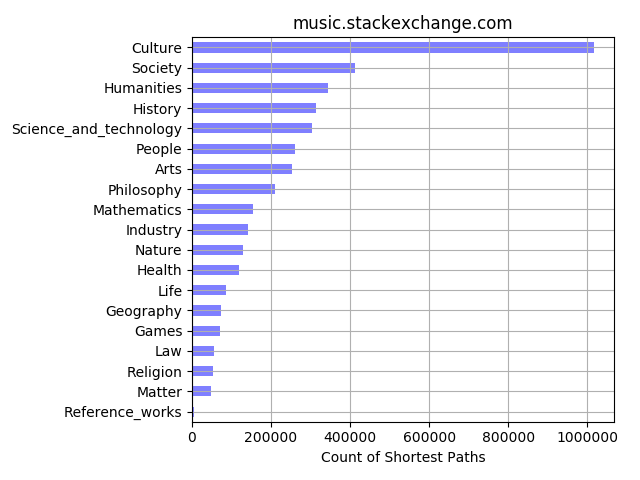
\includegraphics[width=1\linewidth]{imgs/path-counts/music_stackexchange_com}
        \caption{Paths count for Music}
        \label{fig:path-count-music}
    \end{subfigure}
 
     \begin{subfigure}{0.5\textwidth}
    \centering
        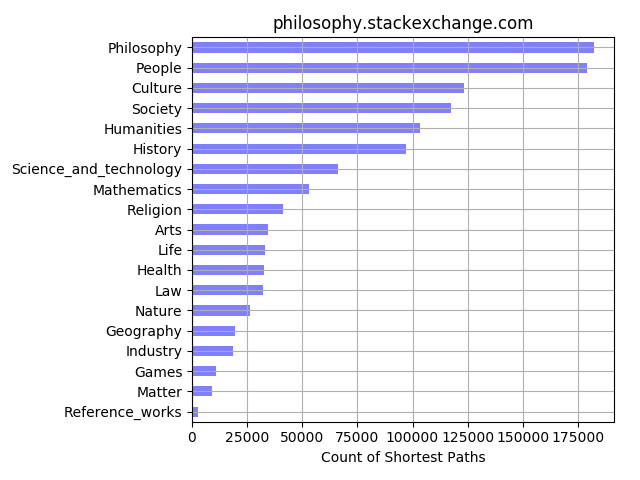
\includegraphics[width=1\linewidth]{imgs/path-counts/philosophy_stackexchange_com}
        \caption{Paths count for Philosophy}
        \label{fig:path-count-philosophy}
    \end{subfigure}%
    \begin{subfigure}{0.5\textwidth}
    \centering
        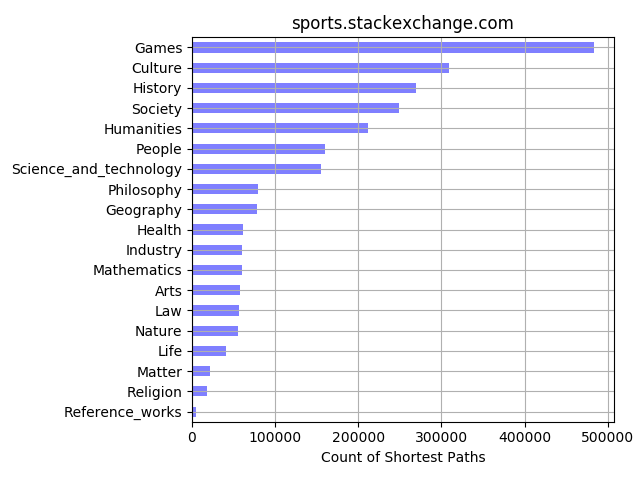
\includegraphics[width=1\linewidth]{imgs/path-counts/sports_stackexchange_com}
        \caption{Paths count for Sports}
        \label{fig:path-count-sports}
    \end{subfigure}
   
 
    \caption{The number of shortest paths through the proposed method. The X-axis shows the number of paths found for each top-level category (displayed on the Y-axis) }
    \label{fig:complete-path-count-distribution}
    
\end{figure}

\begin{figure}[H]
    \centering
	\begin{subfigure}{0.9\textwidth}
    	\centering
        	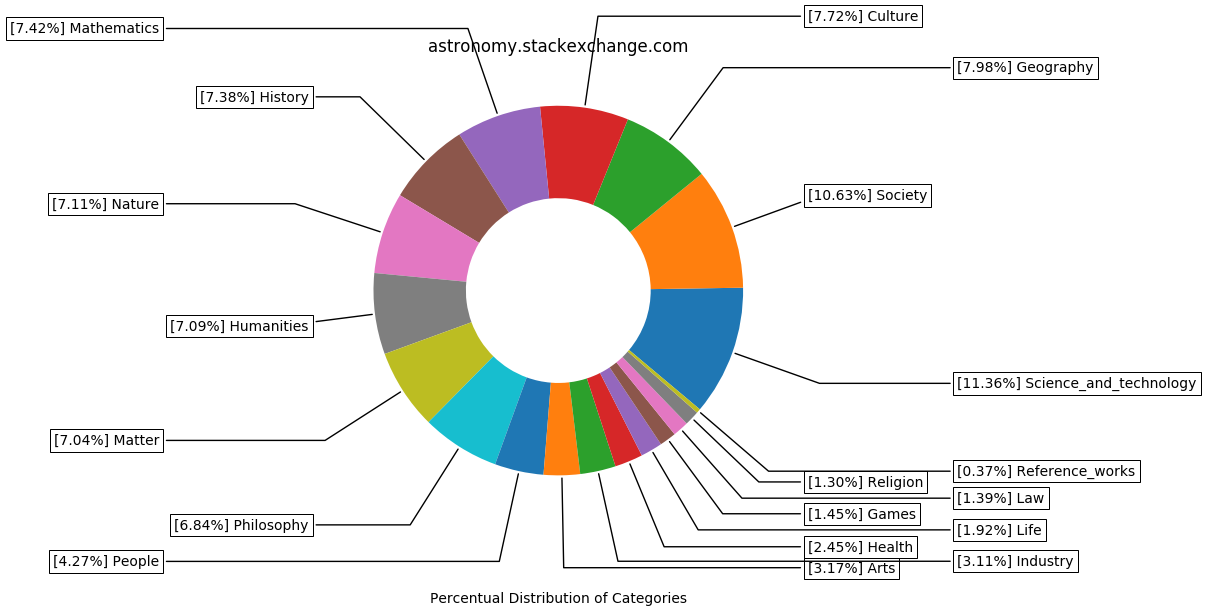
\includegraphics[width=1\linewidth]{imgs/percentual-distribution/astronomy_stackexchange_com_donut}
        	\caption{Percentage distribution of categories for Astronomy}
        	\label{fig:percentage-distribution-astronomy}
    \end{subfigure}%
    
\par\bigskip % 
\par\bigskip % 
	\begin{subfigure}{0.9\textwidth}
    \centering
        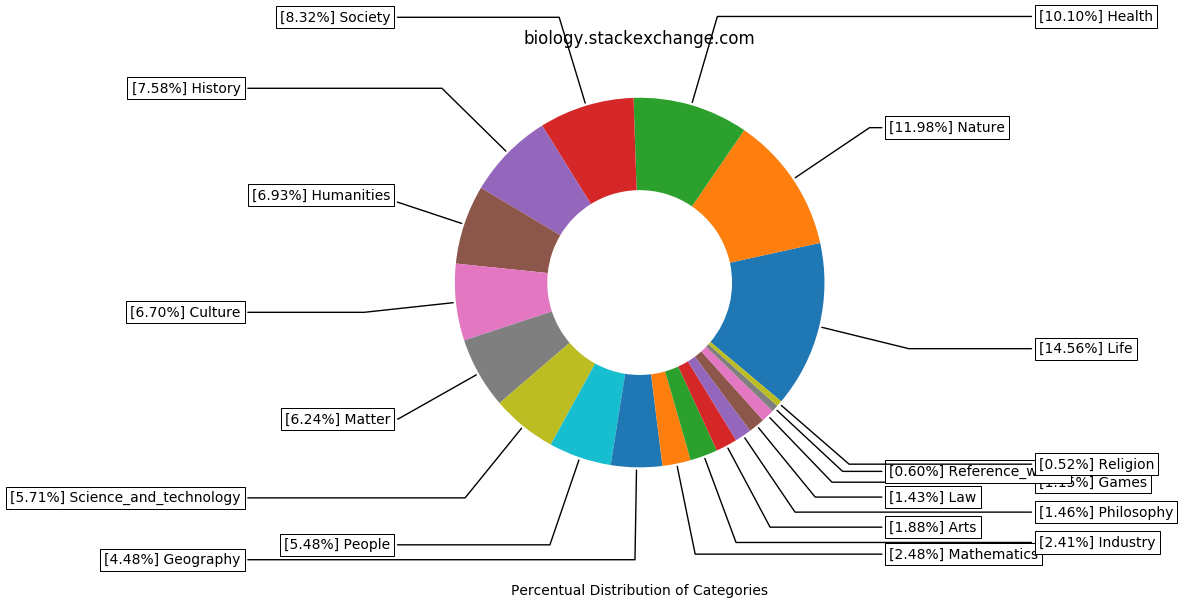
\includegraphics[width=1\linewidth]{imgs/percentual-distribution/biology_stackexchange_com_donut}
        \caption{Percentage distribution of categories for Biology}
        \label{fig:percentage-distribution-biology}
    \end{subfigure}
 
\par\bigskip % 
\par\bigskip % 

	\begin{subfigure}{0.9\textwidth}
    \centering
    	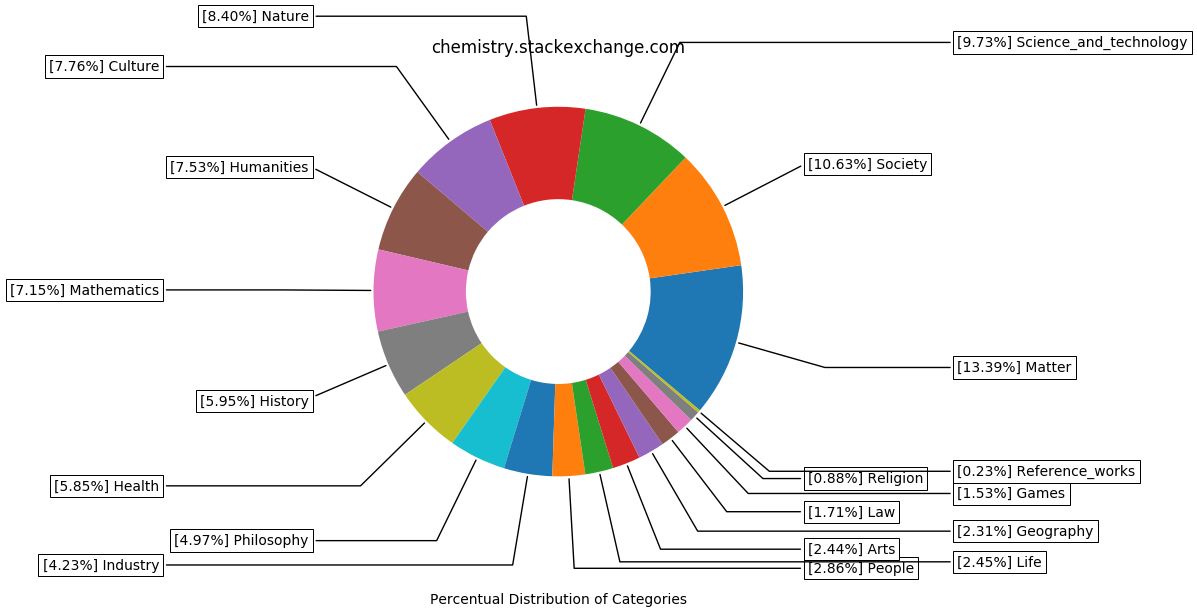
\includegraphics[width=1\linewidth]{imgs/percentual-distribution/chemistry_stackexchange_com_donut}
        \caption{Percentage distribution of categories for Chemistry}
        \label{fig:percentage-distribution-chemistry}
    \end{subfigure}%
\end{figure}
    

\begin{figure}[H]
\ContinuedFloat
\begin{subfigure}{0.9\textwidth}
    \centering
        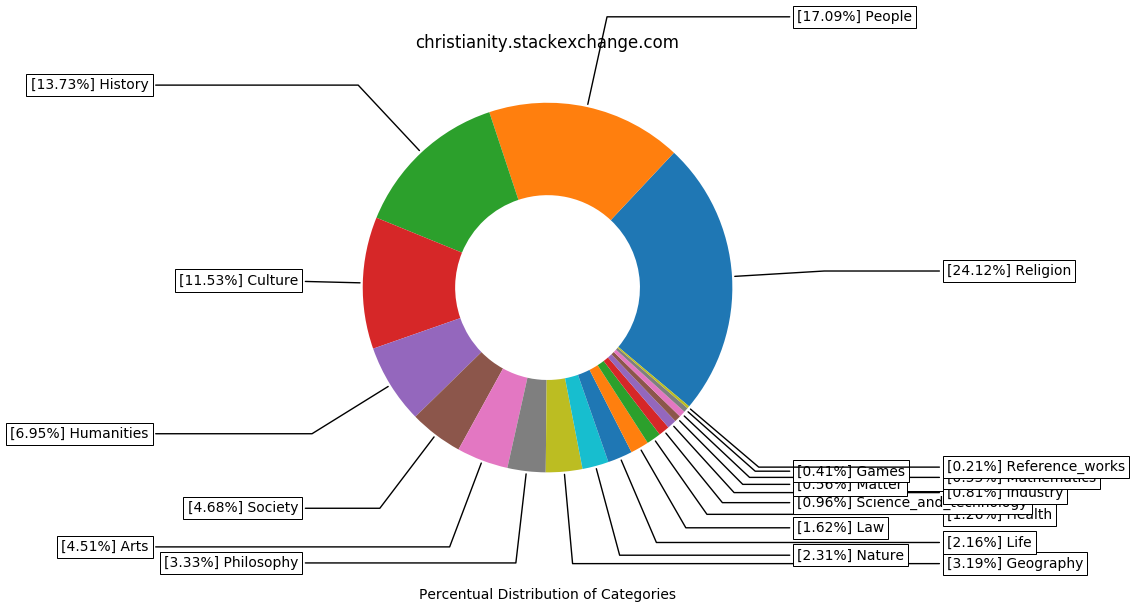
\includegraphics[width=1\linewidth]{imgs/percentual-distribution/christianity_stackexchange_com_donut}
        \caption{Percentage distribution of categories Christianity}
        \label{fig:percentage-distribution-christianity}
    \end{subfigure}
    
     	\par\bigskip % 
    \par\bigskip % 
        
     \begin{subfigure}{0.9\textwidth}
    \centering
        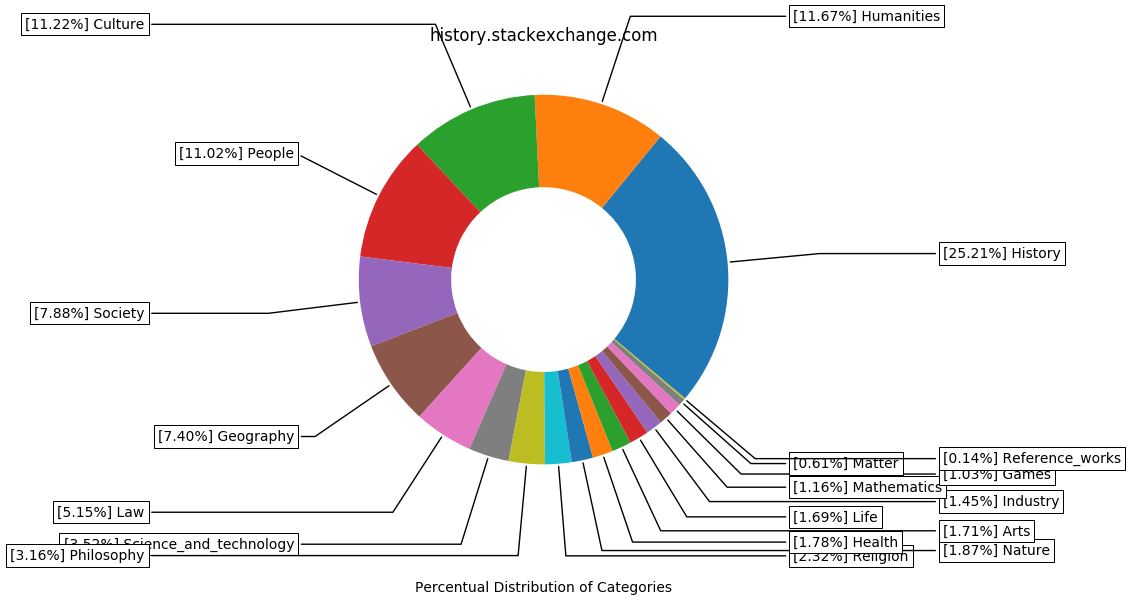
\includegraphics[width=1\linewidth]{imgs/percentual-distribution/history_stackexchange_com_donut}
        \caption{Percentage distribution of categories for History}
        \label{fig:percentage-distribution-history}
    \end{subfigure}%
    
     \par\bigskip % 
    \par\bigskip % 
    \begin{subfigure}{0.9\textwidth}
    \centering
        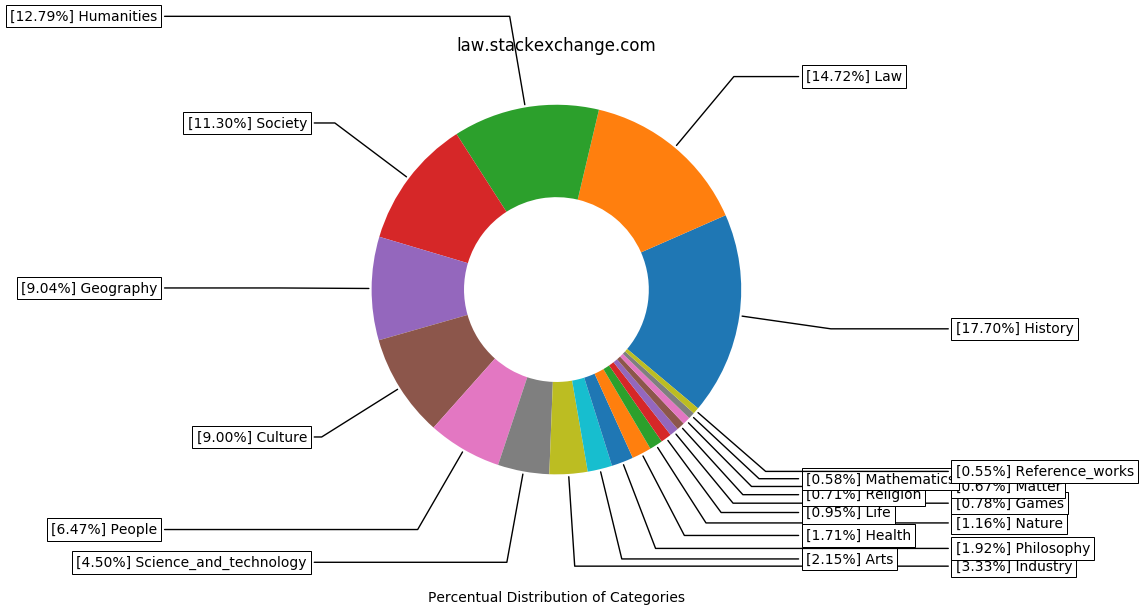
\includegraphics[width=1\linewidth]{imgs/percentual-distribution/law_stackexchange_com_donut}
        \caption{Percentage distribution of categories for Law}
        \label{fig:percentage-distribution-law}
    \end{subfigure} 
 \end{figure}
 
 
\begin{figure}[H]
\ContinuedFloat

    \begin{subfigure}{0.9\textwidth}
    \centering
        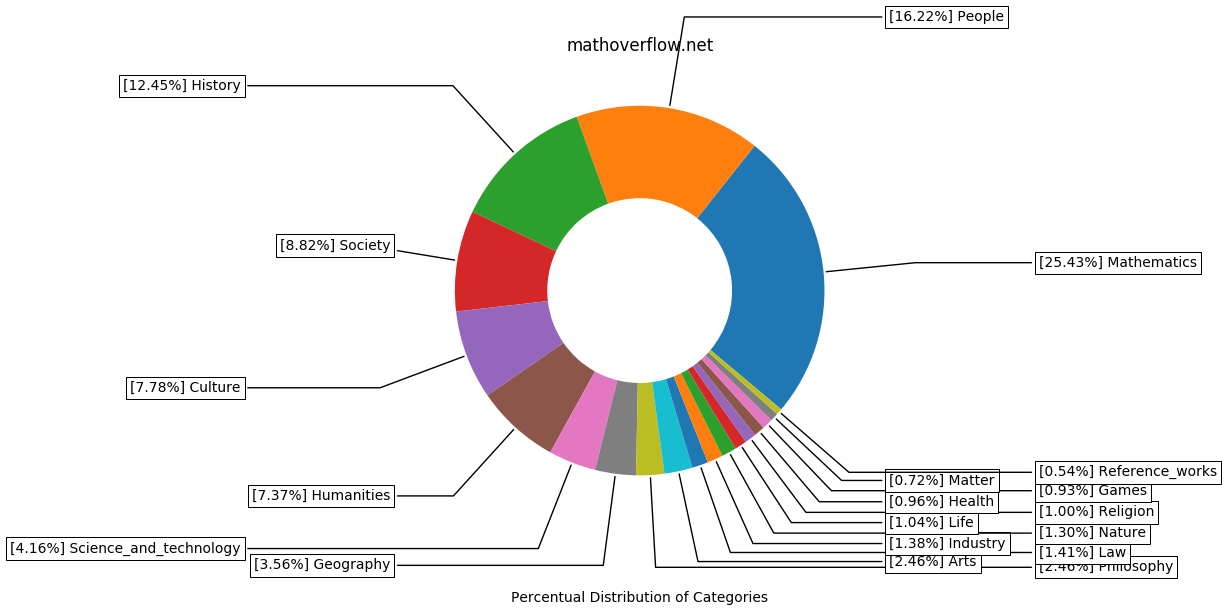
\includegraphics[width=1\linewidth]{imgs/percentual-distribution/mathoverflow_net_donut}
        \caption{Percentage distribution of categories for Math}
        \label{fig:percentage-distribution-math}
    \end{subfigure}%
    
    \begin{subfigure}{0.9\textwidth}
    \centering
        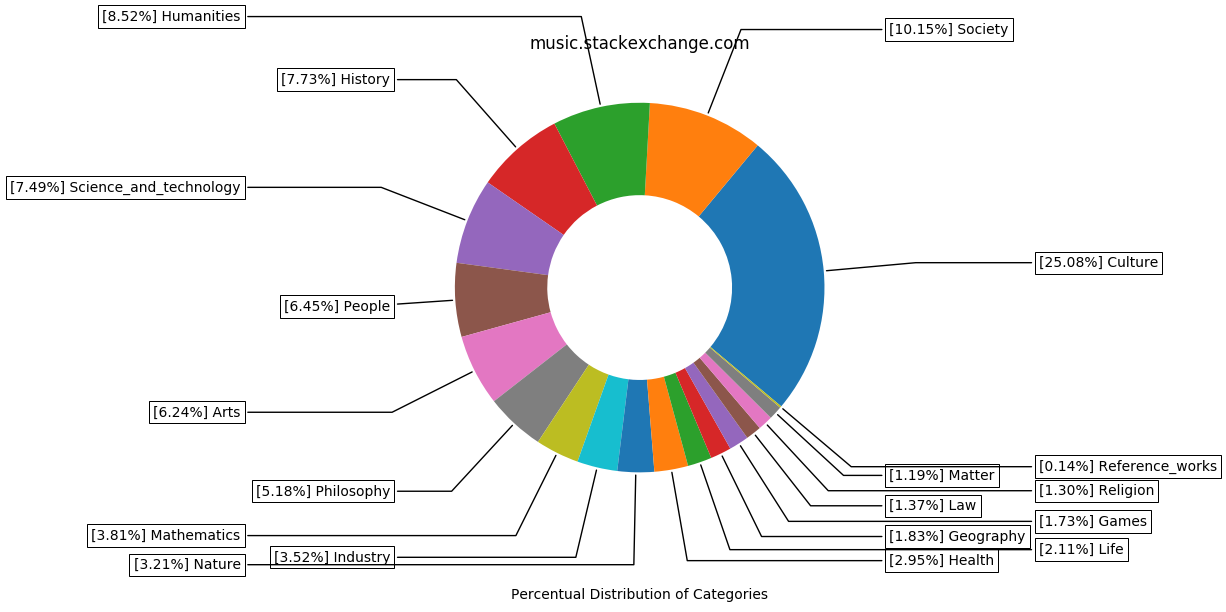
\includegraphics[width=1\linewidth]{imgs/percentual-distribution/music_stackexchange_com_donut}
        \caption{Percentage distribution of categories for Music}
        \label{fig:percentage-distribution-music}
    \end{subfigure}
 
     \begin{subfigure}{0.9\textwidth}
    \centering
        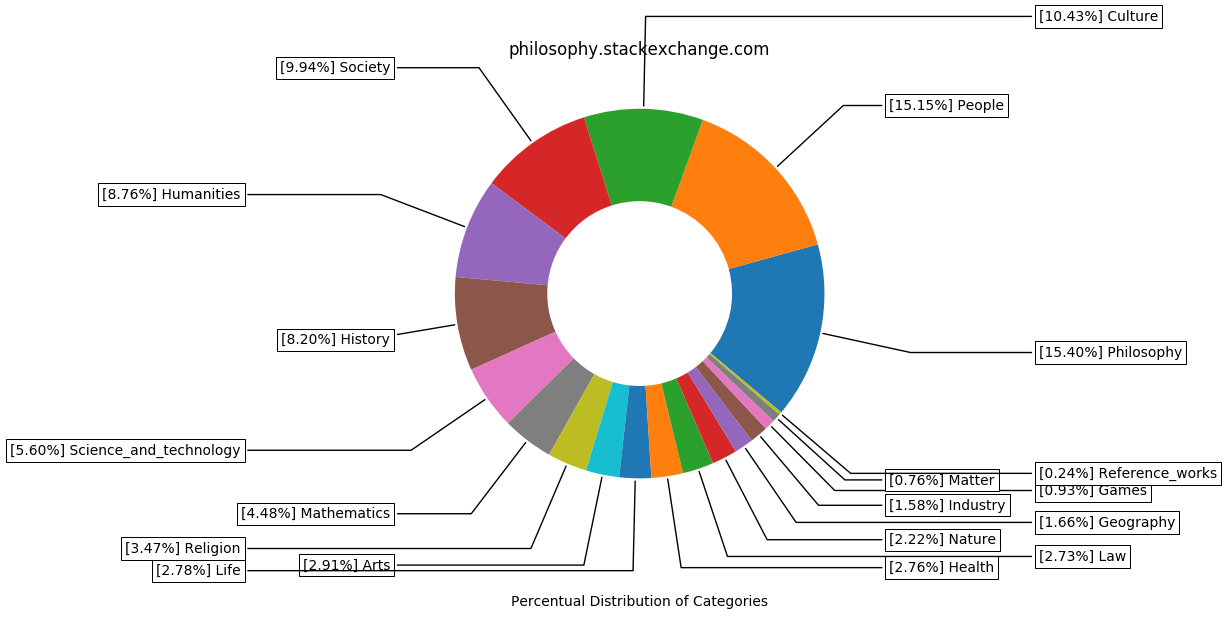
\includegraphics[width=1\linewidth]{imgs/percentual-distribution/philosophy_stackexchange_com_donut}
        \caption{Percentage distribution of categories for Philosophy}
        \label{fig:percentage-distribution-philosophy}
    \end{subfigure}%
 
\end{figure}
 
  
\begin{figure}[H]
\ContinuedFloat

    \begin{subfigure}{0.9\textwidth}
    \centering
        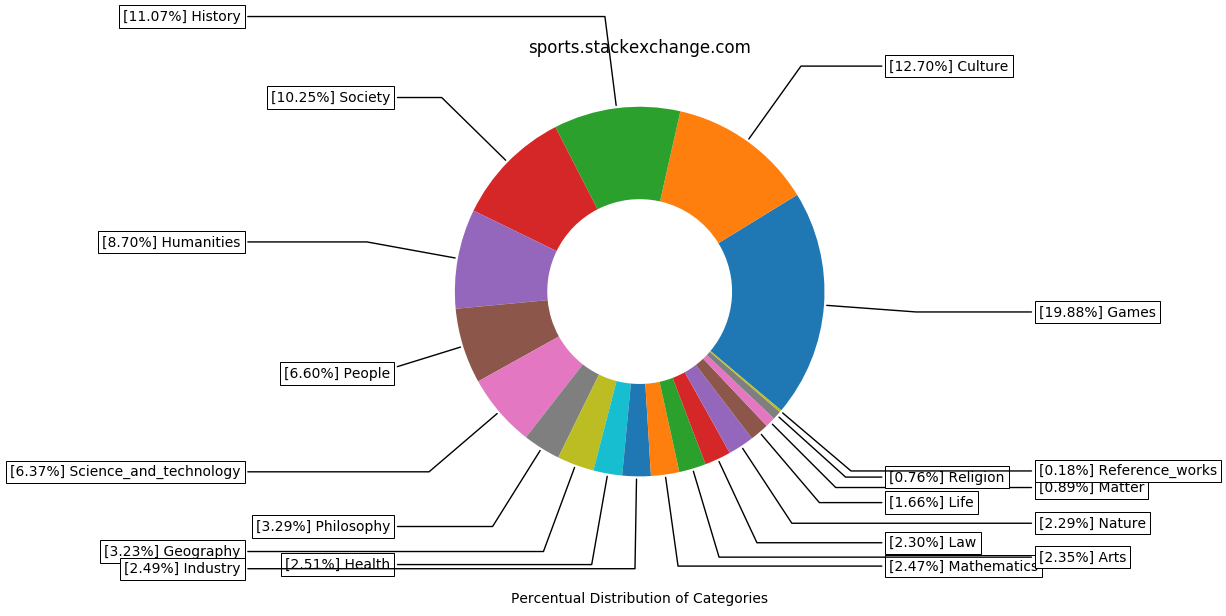
\includegraphics[width=1\linewidth]{imgs/percentual-distribution/sports_stackexchange_com_donut}
        \caption{Percentage distribution of categories for Sports}
        \label{fig:path-sports}
    \end{subfigure}
   
 
    \caption{Percentage distribution of categories for each of the communities evaluated according to the proposed method. }
    \label{fig:complete-percentage-distribution}
    
\end{figure}


\section{\hspace*{3pt} Crowd}

In order to verify if the classification generated by the proposed method is coherent for real users, we conducted an experiment with human judges in order to verify how much they agree with the automatic classification result. For this purpose, we use the stack exchange datasets to make the comparison possible with the experiment described in section \ref{section:proof-of-concept}.



\subsection{\hspace*{3pt} Experimental Design}

Due to the accessibility of established micro-task crowd-sourcing platforms such as Amazon’s Mechanical Turk\footnote{\url{www.mturk.com}} and CrowdFlower, researchers are actively turning toward paid crowd-sourcing to solve data-centric tasks that require human input, such as building ground truths, validating results, and curating data \cite{7156008}.

We used CrowdFlower\footnote{\url{http://crowdflower.com}}, an on-line platform which provides access to a workforce to perform tasks.  It automatically allocates the available tasks to contributors and tests them against known answers, named Gold Standard. Their performance on test questions indicates how much the system trusts each contributor and if they become untrusted, they are removed from the task, and the work is discarded.

For this experiment, we also considered as top-level categories the ones defined as Main topic classifications on Wikipedia (19 categories by the date of data extraction). 

For each one of the ten communities, we run the experiment with 200 different random items extracted from the stack exchange dataset. 

We asked each contributor to read texts randomly chosen from the dataset and answer to what extent the text belongs to each one of the categories on a scale ranging from 0 (not at all) to 3 (to a great extent). 

To alleviate the intensive task of judging for 19 Categories, we asked the participants the evaluate the top-3 categories with greatest percentage distribution and two other random categories.  Figure \ref{fig:example-question} shows a real example of task delivered to contributors for the dataset Biology. The categories LIFE, HEALTH and NATURE are the top-3 categories with the highest degree of membership according to our method (see figures \ref{fig:path-count-biology} and \ref{fig:percentage-distribution-biology}). The categories RELIGION and GAMES were randomly introduced in the survey. 

Random categories were included to validate whether, in addition to agreeing with the categories that appear with the highest distribution in the classification, they also agree with those that do not belong to the most prominent categories.  

Moreover, this mechanism reinforces the verification of the validity of the judgments, since random categories cannot have a distribution of responses similar to those in the top-3 categories.




\begin{figure}[!h]
\centering
  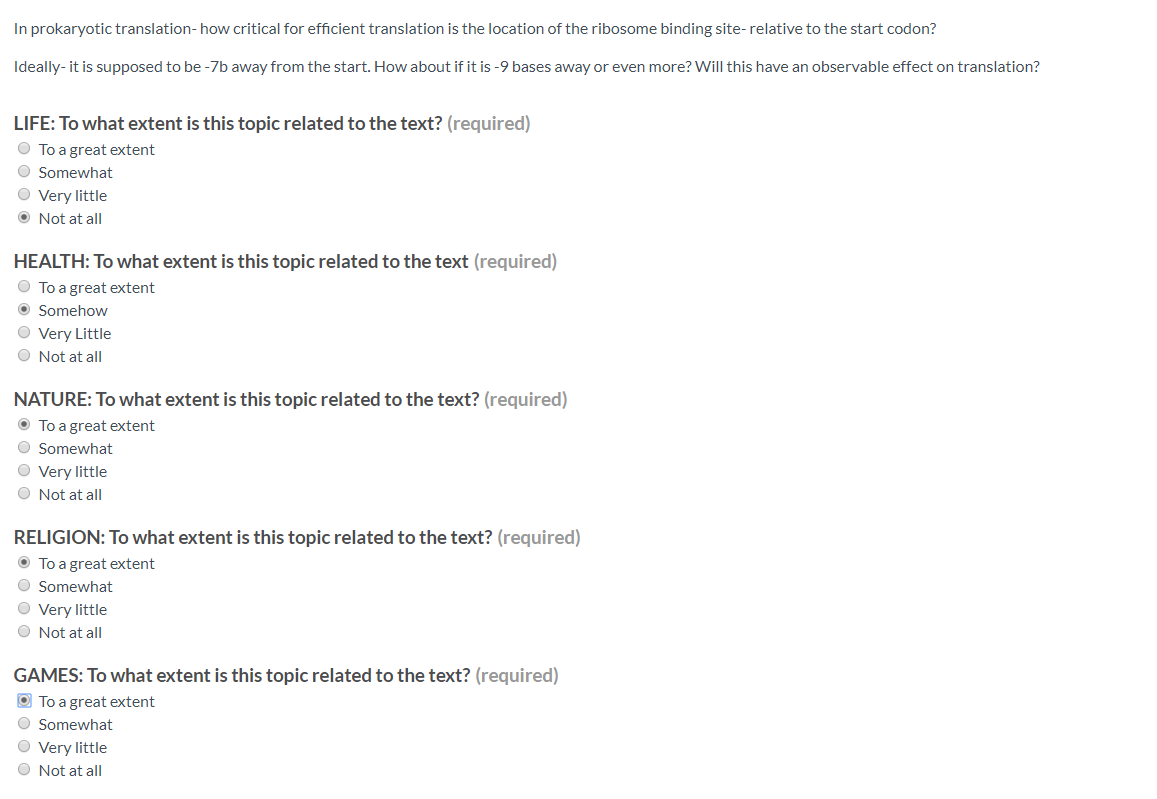
\includegraphics[width=\linewidth]{question-example}
  \caption{Example of task delivered to contributors in the dataset Biology}
  \label{fig:example-question}
\end{figure}

 
To select the participants able to perform the task proposed in the experiment, we created a series of 30 test questions for the stack exchange dataset, so that the participates with low performance in the test questions were eliminated in this stage.


As described in \cite{Gadiraju:2017}, many research works have referred to the importance of task clarity tangentially and stressed the positive impact of task design, clear instructions and descriptions on the quality of crowdsourced work. 

In this regard, we provided a detailed guide for contributors to make sure they clearly understand how to perform the task, with examples of good and bad judgments and also with a description of each one of the 19 categories. To make sure the task is perfectly designed, CrowdFlower platform offers a consulting service where the top-rated contributors evaluate and give feedback on the quality of a given task. An example of the feedback given by this consulting service can be seen in figure \ref{fig:example-feedback}. 

We adjusted the task description according to the suggestions in the feedback by providing more and contextualized examples, as well as explaining, for each test question, the reason why the alternatives were considered wrong or correct.  

\begin{figure}[!h]
\centering
  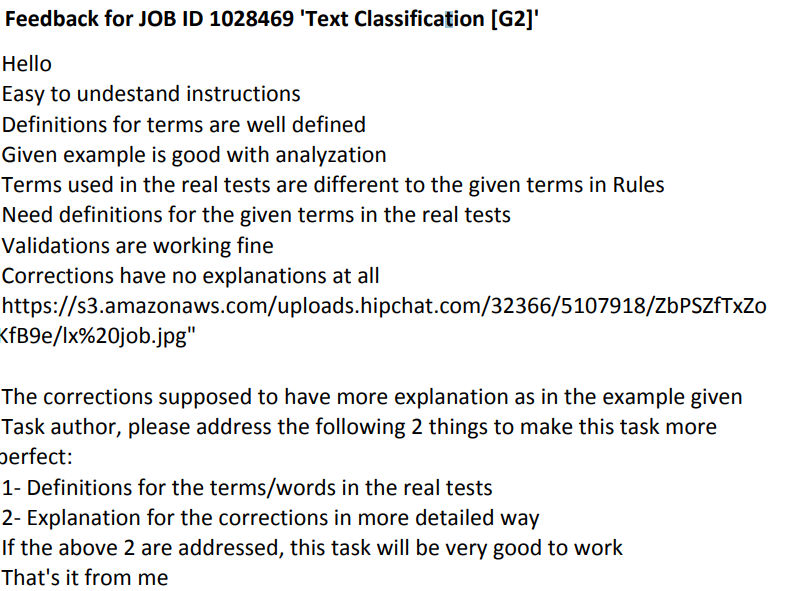
\includegraphics[width=\linewidth]{crowd-feedback}
  \caption{Example of feedback given by the consulting service provided by CrowdFlower platform}
  \label{fig:example-feedback}
\end{figure}


in the final experiment, 1265 unique contributors participated from June to August of 2018. The overall setup for the experiment is presented in table \ref{tab:experiment-overview}. A trusted judgment is an answer from a contributor with an accuracy score higher than the minimum accuracy considered for this experiment (0.75), while an untrusted judgment is an answer from a contributor whose accuracy score has fallen below this value.

\begin{table}[!h]

\centering
\caption{Overall setup for the experiment with crowd workers}
\label{tab:experiment-overview}
\resizebox{\textwidth}{!}{%
\begin{tabular}{@{}llllll@{}}
\toprule
Community         & Trusted Judgments & Untrusted Judgments & Average Judgments per Row & Average Trust of Workers & Unique Workers \\ \midrule
Astronomy         & 640               & 36                  & 3.2000                    & 0.8651                   & 128            \\
Biology (Elite)   & 612               & 48                  & 3.0600                    & 0.8390                   & 122            \\
Biology (Regular) & 1040              & 278                 & 5.2000                    & 0.8366                   & 208            \\
Chemistry         & 751               & 12                  & 3.7550                    & 0.8197                   & 150            \\
Christianity      & 628               & 16                  & 3.1558                    & 0.8843                   & 125            \\
History           & 602               & 76                  & 3.0251                    & 0.7997                   & 120            \\
Law               & 601               & 0                   & 3.0050                    & 0.8831                   & 120            \\
Math              & 630               & 32                  & 3.1500                    & 0.9306                   & 126            \\
Music             & 602               & 28                  & 3.0100                    & 0.9137                   & 120            \\
Philosophy        & 717               & 108                 & 3.5850                    & 0.8376                   & 143            \\
Sports            & 629               & 32                  & 3.1608                    & 0.8349                   & 125            \\ \bottomrule
\end{tabular}%
}
\end{table}

\subsection{\hspace*{3pt} Elite Contributors X Regular Contributors}

Before we run the experiment with all ten communities, we first evaluated whether there is a difference between the quality of judgments performed by elite contributors and the judgments made by regular contributors. The elite contributors (also called level-3 contributors in the context of CrowdFlower platform) are those who completed over 100 test questions across hundreds of different types of tasks and have a near perfect overall accuracy. To perform this verification, we ran the experiment using the Biology dataset in two different groups: one only with regular contributors and the other with level-3 contributors. They were asked to judge the same set of 200 questions. 

A statistical test was applied aiming at determining if the results obtained in the answers given by the two groups can be considered significantly different from each other. The Wilcoxon-Mann-Whitney nonparametric statistical inference test was applied\cite{feltovich2003nonparametric}. This test compares the mean of two independent samples and does not require normality and homoscedasticity in the series of values compared. The level of significance was set at 95\%. The p-value evaluates the result of this statistical test. The lower is the p-value, the higher the significance of the outcome. For a significance level of 95\%, if the p-value is smaller than 0.05, we can conclude that responses observed for the two groups are distinct. 

We obtained a p-value of  0.267, meaning that there is no significant difference between the answers given by the two groups. 

If we analyze the table \ref{tab:experiment-overview} it is possible to see that regular users are less efficient and thus more judgments are needed to achieve a reasonable level of agreement. 

Even though the price paid to regular contributors is lower in comparison to elite contributors, we decided to admit only level-3 users.

\subsection{\hspace*{3pt} Quality Control}

While dealing with a random collection of strangers to perform relevance evaluation, two primary concerns have risen:  i) How to ensure that contributors performing the evaluation will have the necessary skill or knowledge? ii) How to make sure that the contributors will make a high-quality effort to do the work, rather than clicking randomly on the responses?

 
To address these questions, we defined some parameters of quality regarding the contributors and the experiment:

\begin{enumerate}

\item We restricted the participation to contributors from English-speaking countries to ensure that they understood the task and instructions adequately. 

\item We restricted the participation to Level-3 contributors on CrowdFlower, meaning that only those who completed over 100 test questions across hundreds of different types of tasks and have a near perfect overall accuracy. They are contributors of the highest quality on CrowdFlower.

\item We restricted each contributor to a maximum of five judgments across all datasets, to minimize the number of contributors trying to complete a massive number of tasks in order to make more money 

\item We predefined the minimum of 0.75 regarding the level of agreement among the contributors for each row of text evaluated. In case a row does not reach this value with the default number of 3 judgments, new judgments were requested until the agreement coefficient reached 0.75.

\end{enumerate}

\subsection{\hspace*{3pt} Results and Discussion}



 \begin{figure}[H]
    \centering
    \begin{subfigure}{0.5\textwidth}
    \centering
        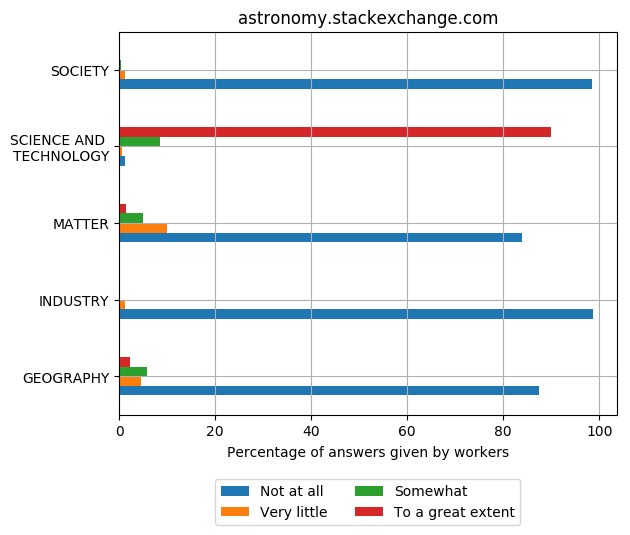
\includegraphics[width=1\linewidth]{imgs/crowd-results/astronomy_stackexchange_com}
        \caption{Distribution of Answers for Astronomy}
        \label{fig:crowd-results-astronomy}
    \end{subfigure}%
    \begin{subfigure}{0.5\textwidth}
    \centering
        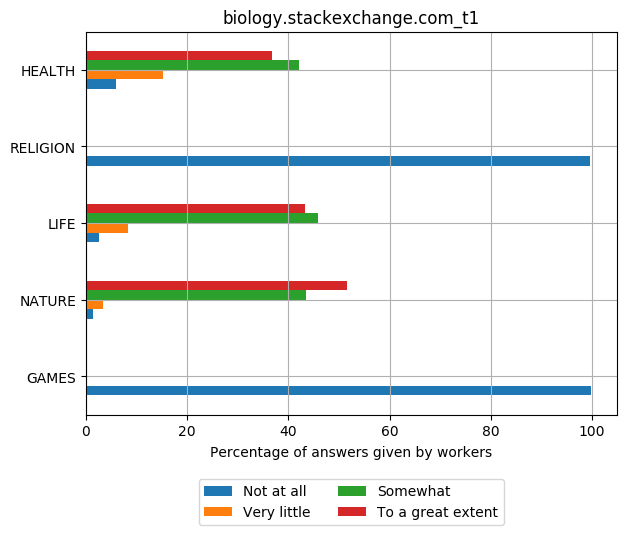
\includegraphics[width=1\linewidth]{imgs/crowd-results/biology_stackexchange_com_t1}
        \caption{Distribution of Answers for Biology (Regular)}
        \label{fig:crowd-results-biology-1}
    \end{subfigure}
 
     \begin{subfigure}{0.5\textwidth}
    \centering
        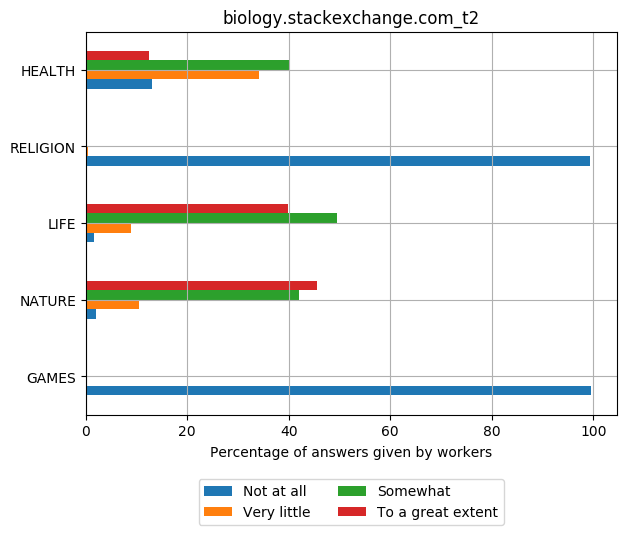
\includegraphics[width=1\linewidth]{imgs/crowd-results/biology_stackexchange_com_t2}
        \caption{Distribution of Answers for Biology (Elite)}
        \label{fig:crowd-results-biology-2}
    \end{subfigure}%
    \begin{subfigure}{0.5\textwidth}
    \centering
        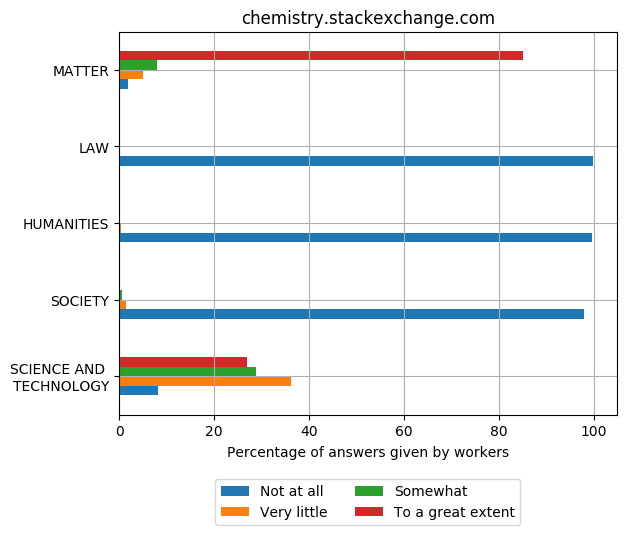
\includegraphics[width=1\linewidth]{imgs/crowd-results/chemistry_stackexchange_com}
        \caption{Distribution of Answers for Chemistry}
        \label{fig:crowd-results-chemistry}
    \end{subfigure}

        
     \begin{subfigure}{0.5\textwidth}
    \centering
        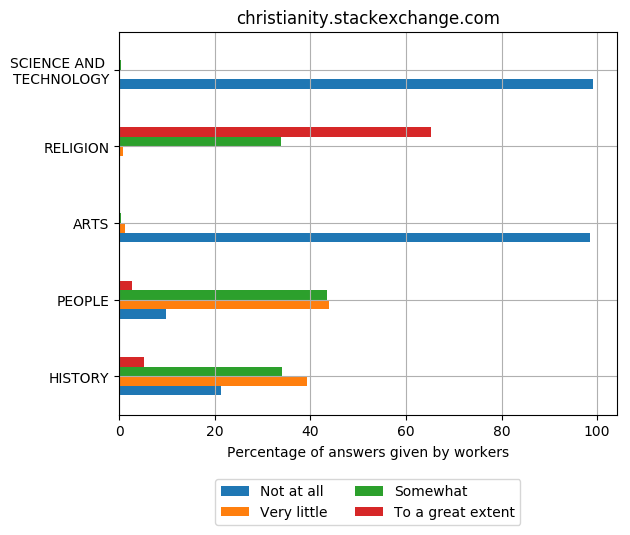
\includegraphics[width=1\linewidth]{imgs/crowd-results/christianity_stackexchange_com}
        \caption{Distribution of Answers for Christianity}
        \label{fig:crowd-results-christianity}
    \end{subfigure}%
    \begin{subfigure}{0.5\textwidth}
    \centering
        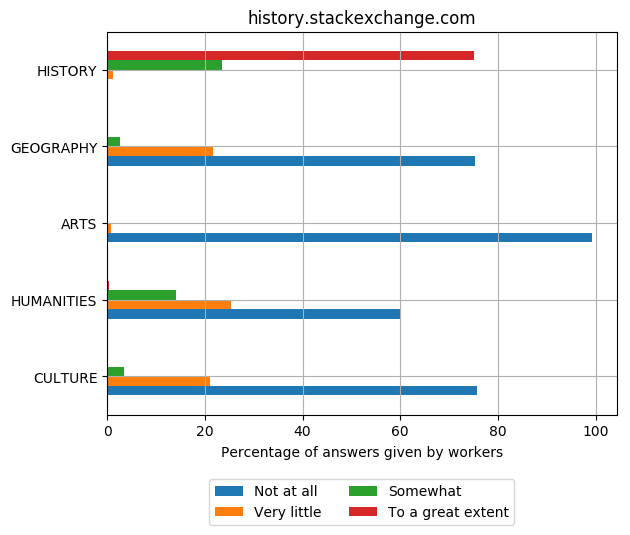
\includegraphics[width=1\linewidth]{imgs/crowd-results/history_stackexchange_com}
        \caption {Distribution of Answers for  History}
        \label{fig:crowd-results-history}
    \end{subfigure} 

    \end{figure}
    
 \begin{figure}[H]
 \ContinuedFloat
    \centering
    \begin{subfigure}{0.5\textwidth}
    \centering
        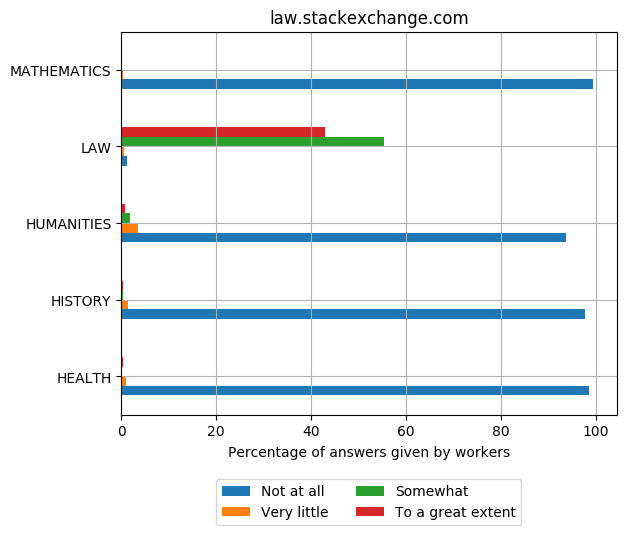
\includegraphics[width=1\linewidth]{imgs/crowd-results/law_stackexchange_com}
        \caption{Distribution of Answers for Law}
        \label{fig:crowd-results-law}
    \end{subfigure}%
    \begin{subfigure}{0.5\textwidth}
    \centering
        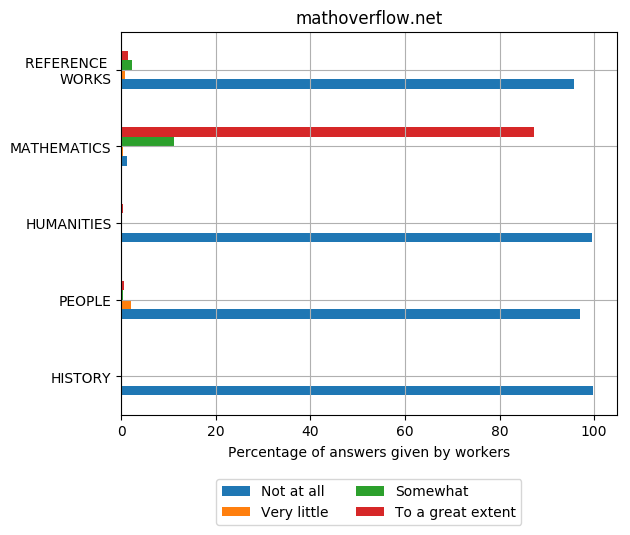
\includegraphics[width=1\linewidth]{imgs/crowd-results/mathoverflow_net}
        \caption{Distribution of Answers for Math}
        \label{fig:crowd-results-math}
    \end{subfigure}
 
     \begin{subfigure}{0.5\textwidth}
    \centering
        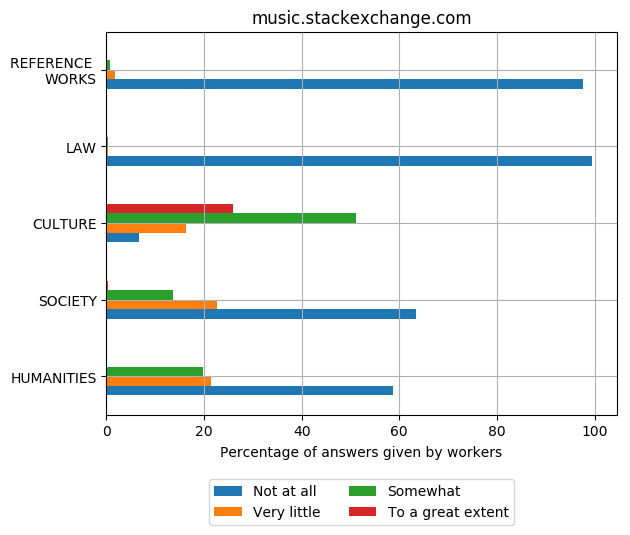
\includegraphics[width=1\linewidth]{imgs/crowd-results/music_stackexchange_com}
        \caption{Distribution of Answers for Music}
        \label{fig:crowd-results-music}
    \end{subfigure}%
    \begin{subfigure}{0.5\textwidth}
    \centering
        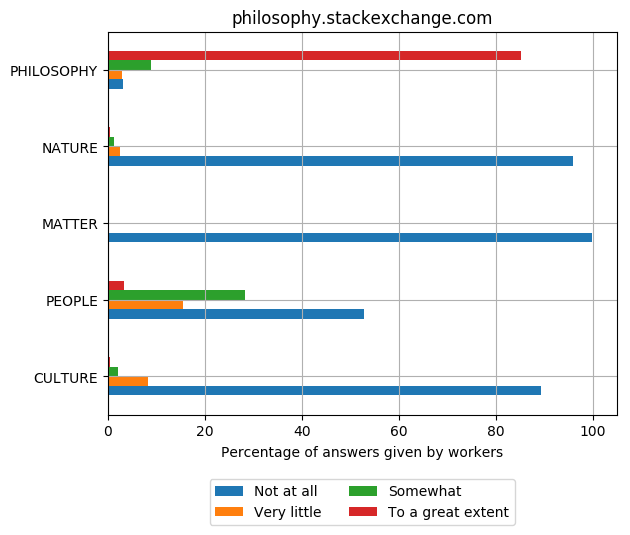
\includegraphics[width=1\linewidth]{imgs/crowd-results/philosophy_stackexchange_com}
        \caption{Distribution of Answers for Philosophy}
        \label{fig:crowd-results-philosophy}
    \end{subfigure}
    
     \begin{subfigure}{0.5\textwidth}
    \centering
        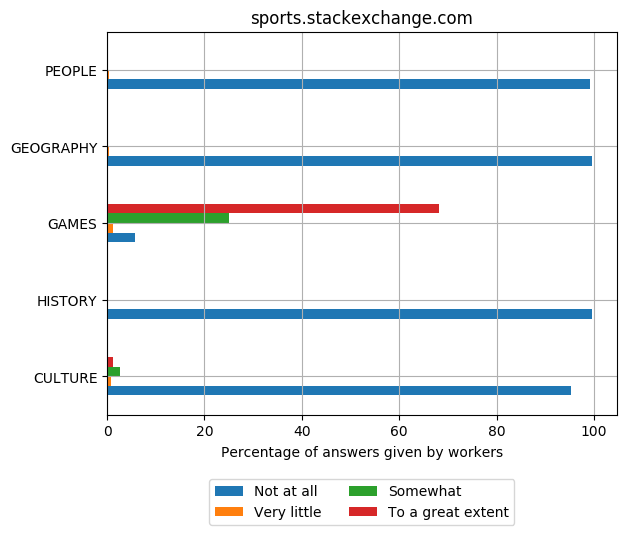
\includegraphics[width=1\linewidth]{imgs/crowd-results/sports_stackexchange_com}
        \caption{Distribution of Answers for Sports}
        \label{fig:crowd-results-sports}
    \end{subfigure}%
 \caption{Percentage distribution of answers given by crowd contributors for each one of the ten communities evaluated }
    \label{fig:complete-crowd-distribution}
    
\end{figure}


    \chapter{\hspace*{3pt} Related Works}
\label{chapter:related-works}


The knowledge encoded in Wikipedia has being used by many researchers as a tool for performing several tasks, including text categorization \cite{Gabrilovich:2006}, co-reference resolution \cite{strube2006wikirelate}, predicting document topics \cite{schonhofen2009identifying}, automatic word sense disambiguation \cite{mihalcea2007using}, searching synonyms \cite{krizhanovsky2006synonym} and computing semantic relatedness 
\cite{ponzetto2006exploiting}, \cite{gabrilovich2007computing}, \cite{milne2007computing}.

For better comprehension, we described the researches studied grouped as follows: 

\begin{enumerate}
\item Researches dedicated to understanding and describing the Wikipedia’s latent category structure.
\item Researches that exploit  Wikipedia knowledge to determine the content of textual resources.
\item Researches that use information extracted from Wikipedia to create text classifiers.
\end{enumerate}


\section{\hspace*{3pt}Wikipedia Category Structure}

The articles in Wikipedia are associated with one or more categories, and the categories are linked together forming a latent structure. This structure is created and curated by volunteers, meaning that the quality of reliability of this structure is dependent on the knowledge of the contributors.

The method proposed in this thesis aims at categorizing text-based resources based on the Named Entities found on the text and its relation to a set of predefined categories in Wikipedia. We use the Wikipedia category structure as a graph and determine the categorization based on the  shortest paths between the categories associated with the entities and a set of more generic predefined Wikipedia categories. We have studied two projects that focus on explaining Wikipedia’s category structure and the types of relationships between category: 


\begin{enumerate}

\item Decoding Wikipedia Categories for Knowledge Acquisition \cite{nastase2008decoding} which tries to understand the conceptual relationships between categories.
\item Extracting Semantic Relationships between Wikipedia Categories \cite{chernov2006extracting} which concentrates on the deriving semantic relationships within the categories in the graph.

\end{enumerate}


Because humans create it, the structure of categories can vary depending on the people who are involved in the process. The work described in \cite{nastase2008decoding} is a project to automatically understand the structure of categories created by contributors. It classifies the types of relationship between the categories, based on the purpose of these relationships. This project focuses on relationship types represented in links between categories and articles, and between categories. Two links within the category structure can represent similar relationship types without having similar category names. Thus, an automatic approach for representing the category links in a standardized way
was created in \cite{nastase2008decoding} .

The project described in \cite{chernov2006extracting} analyzes the connections within the category structure aiming to automatically derive semantic features from Wikipedia categories. Project \cite{chernov2006extracting} covers an implementation for finding articles with the same meaning by looking at the category links in Wikipedia’s category structure. The semantic similarity for an article is found by creating a \gls{scs} which represents the semantic connection to other articles. Their result is a semantic schema that retrieves the most relevant articles for a given word, without considering the word’s syntax.

Both of these projects provide useful information about the category structure and contain relevant ideas for further implementation.



%\cite{halavais2008analysis} quantitatively compared the distribution of 3,000 Wikipedia articles coded into Library of Congress categories with a distribution of published books. They found substantial overlap between Wikipedia categories and topics from other encyclopedias, however, the number of articles sampled and categories examined was relatively small.
%\cite{kittur2009s} demonstrated a simple technique for determining the distribution of topics for articles in Wikipedia, mapping all items to the top categories. The process was based on building the Category Graph of Wikipedia and counting the edges on the shortest paths from the categories of an article to the top categories of Wikipedia. 
%\cite{farina2011automatically} improved this by penalizing edges followed in the wrong direction concerning the hierarchy. They were able to account for the orientation of the categories assignments, without losing information, and showed to outperform the original method, measured as the similarity with manually generated assignments.
%\cite{strube2006wikirelate} developed a system named WikiRelate!. They used data from Wordnet, Wikipedia, and Google for computing degrees of semantic similarity and reported that Wikipedia outperforms Wordnet.  They used different measures for computing semantic relatedness and showed good results with the one based on paths. The success of their experiments gives support to our method, which also utilizes the Wikipedia Graph. 



\section{\hspace*{3pt}Wikipedia as Knowledge Base}


Our primary goal is to categorize textual resources based on the set of categories of Wikipedia structure. This task requires a way of extracting features from Wikipedia.
There are many projects with the goal of identifying Wikipedia entries in text and taking advantage of the Wikipedia’s encyclopedic knowledge since Wikipedia is a massive resource of encyclopedic knowledge. Some of these projects identified in this research are: 

\begin{itemize}

\item  Entity Extraction, Linking, Classification, and Tagging for Social Media: A Wikipedia-based Approach \cite{gattani2013entity} which extracts Wikipedia article titles
in tweets for understanding their content.

\item Large-Scale Taxonomy Mapping for Restructuring and Integrating Wikipedia\cite{ponzetto2009large}: The approach presented in this project use WordNet subsumption hierarchy, to perform category disambiguation and taxonomy restructuring in Wikipedia structure.

\item Overcoming the Brittleness Bottleneck using Wikipedia: Enhancing Text Categorization with Encyclopedic Knowledge \cite{Gabrilovich:2006}.

\end{itemize}

The research described in \cite{ponzetto2009large} provides an extension to WordNet. It takes advantage of the semantic information from synsets to generate automatically derive a  taxonomy.

The project’s method uses WikiTaxonomy, a taxonomy based on Wikipedia, and improve it by linking the entries in the taxonomy to the synset from WordNet. These results are used to generate a new and improved Wikipedia taxonomy.

Encyclopedic knowledge from Wikipedia is also found in \cite{Gabrilovich:2006}. This project creates a classifier that is extended with knowledge from Wikipedia. The authors assume that each Wikipedia article represents a concept and that documents can be classified under a feature space of Wikipedia concepts.

The research presented in \cite{gattani2013entity} creates a category-based classifier that relies on knowledge from Wikipedia. This project has a goal very similar to ours: to categorize tweets based on their textual content.

The solution implemented for this problem uses Wikipedia as a knowledge base, where Wikipedia articles are connected to concepts used in the classification process.


\section{\hspace*{3pt}Classifiers Based on Wikipedia}

The approach described in this thesis is a category-based classifier, which classifies textual resources based on the relation of the text being classified and a set o predefined categories on Wikipedia. Classifiers can be created in many forms, and the classifiers can focus on different features. We have studied some projects which creates classifiers from Wikipedia:
\begin{enumerate}

\item What's in Wikipedia?: mapping topics and conflict using socially annotated category structure \cite{kittur2009s}
\item Identifying document topics using the Wikipedia category network \cite{schonhofen2009identifying}  
\item Entity Extraction, Linking, Classification, and Tagging for Social Media: A Wikipedia-based Approach \cite{Gabrilovich:2006}.
\end{enumerate}



The method proposed by Kittur and Chi \cite{kittur2009s} is also similar to our approach. 
Their goal is to automatically assign a Wikipedia article to a set of what they call macro-categories (A subset of Wikipedia categories that is in the top of the hierarchy) 
The main difference is that their approach is limited to articles inside Wikipedia, and cannot be generalized for other text-based resources. 


Other similar work regarding our approach is the research presented in  \cite{schonhofen2009identifying} . This project is closely related to our research, with a similar goal: to determine whether documents can be categorized by only exploring titles and categories of Wikipedia articles.

The main difference between this project and our approach is the choice of output categories in the final classification. The authors categorizes documents to a broader number of Wikipedia categories, while we categorize documents to a set of predefined, more generic group of categories. Their categorization approach are similar to ours, and consists of two main steps:
1. Look for word compounds within the text that match processed titles of Wikipedia articles.
2. Retrieve the Wikipedia articles’ categories.

The classifier in \cite{schonhofen2009identifying} is a term-based classifier also similar to our approach, but the keywords are categorized to the corresponding Wikipedia articles’ categories instead of an independent category set. Another difference is that we look at the whole category structure, while \cite{schonhofen2009identifying} looks at categories retrieved from the matched Wikipedia article titles, hence it is more limited. 

Another term-based classifier is found in \cite{Gabrilovich:2006}, which is a project for classifying and tagging tweets. The project uses Wikipedia to create a knowledge base, where they process titles of Wikipedia articles and link them towards suitable categories representing the content of their article.



\subsection{\hspace*{3pt} Evaluation of Classifiers}

The evaluation measures for the classifiers presented in \cite{schonhofen2009identifying} and  \cite{Gabrilovich:2006} have been precision, recall, and F1-Score. The researchers also presented the micro-average evaluation, which means that they take the measures individually for each class.

It is relevant to analyze what the classifiers described in this section evaluated so that we can compare our results
with the results of other classifiers. 

The evaluation of \cite{schonhofen2009identifying} is divided into two experiments: 

\begin{enumerate}

\item Classification of Wikipedia articles based on their text bodies.
\item Classification of two independent corpora: 20 Newsgroups and RCV1.making it suitable for comparison with our approach.

\end{enumerate}


The categorization evaluation of \cite{gattani2013entity} is based on topics within the tweets.

Since the authors did not use the set of categories and also added information to their knowledge
base from other places external to Wikipedia, which means that their classes are broader and not suitable for comparison. 

Kittur and Chi \cite{kittur2009s} evaluated the approach by comparing the attributions made by their method with the judgment of human raters. Although they preset a good correlation between the method and the judgments, the experiment was realized in a very small scale. 


    \chapter{\hspace*{3pt} Conclusion}
\label{chapter:conclusion}


	\begin{appendices}
  \chapter{Wikipedia Category Graph - Nodes Dataset}
  \label{app:dataset-categories}
  
\scriptsize
\setlength\LTleft{0pt}
\setlength\LTright{0pt}
\rowcolors{2}{}{tblO}
\begin{longtable}{@{}lllllll@{}}
\caption{A sample including the 50 first rows of the dataset generated from the Wikipedia Category Graph. Each row represent one node of the graph along with its Degree, Clustering Coefficient, and Centrality information  }
\label{table:wcg-dataset}\\
\toprule
CategoryName & Degree & Outdegree & Indegree & Clustering Coefficient& Betweenness Centrality& PageRank \\* \midrule
\endfirsthead
%
\multicolumn{7}{c}%
{{\bfseries Table \thetable\ continued from previous page}} \\
\toprule
CategoryName & Degree & Outdegree & Indegree & Clustering Coefficient& Betweenness Centrality& PageRank \\* \midrule
\endhead
%
\bottomrule
\endfoot
%
\endlastfoot
%
Futurama & 15 & 11 & 4 & 0.00909090909090909 & 5,89E+08 & 4,27E+08 \\
World\_War\_II & 52 & 15 & 37 & 0.047619047619047616 & 2,72E+11 & 1,05E+11 \\
Programming\_languages & 56 & 5 & 51 & 0.15 & 9,48E+08 & 8,17E+08 \\
Professional\_wrestling & 27 & 4 & 23 & 0.0 & 2,02E+10 & 8,64E+09 \\
Algebra & 16 & 1 & 15 & 0.0 & 1,26E+09 & 7,42E+10 \\
Anime & 34 & 8 & 26 & 0.05357142857142857 & 1,66E+09 & 4,01E+09 \\
Abstract\_algebra & 32 & 3 & 29 & 0.16666666666666666 & 7,26E+07 & 3,98E+08 \\
Mathematics & 29 & 7 & 22 & 0.14285714285714285 & 1,54E+07 & 1,33E+11 \\
Linear\_algebra & 18 & 2 & 16 & 0.0 & 6,04E+08 & 1,25E+11 \\
Calculus & 11 & 3 & 8 & 0.5 & 4,42E+07 & 9,90E+08 \\
Monarchs & 36 & 6 & 30 & 0.16666666666666666 & 8,12E+09 & 4,73E+08 \\
British\_monarchs & 16 & 7 & 9 & 0.09523809523809523 & 2,43E+08 & 6,87E+08 \\
Star\_Trek & 28 & 9 & 19 & 0.027777777777777776 & 2,72E+09 & 1,57E+10 \\
People & 360 & 3 & 357 & 0.3333333333333333 & 9,76E+08 & 0.00032288729268168 \\
Popes & 47 & 18 & 29 & 0.0196078431372549 & 5,80E+08 & 2,59E+10 \\
Desserts & 23 & 2 & 21 & 0.5 & 4,16E+07 & 1,96E+10 \\
Fruit & 28 & 4 & 24 & 0.25 & 3,34E+08 & 2,71E+09 \\
Lists & 33 & 4 & 29 & 0.16666666666666666 & 1,92E+11 & 6,54E+09 \\
Computer\_science & 21 & 7 & 14 & 0.2619047619047619 & 7,98E+09 & 6,61E+09 \\
The\_Simpsons & 18 & 9 & 9 & 0.027777777777777776 & 1,69E+09 & 7,97E+08 \\
Algorithms & 58 & 6 & 52 & 0.06666666666666667 & 9,51E+08 & 4,56E+09 \\
Data\_structures & 24 & 6 & 18 & 0.13333333333333333 & 9,86E+07 & 1,25E+09 \\
Monty\_Python & 15 & 4 & 11 & 0.0 & 2,56E+07 & 6,11E+08 \\
Middle-earth\_places & 0 & 0 & 0 & 0.0 & 0.0 & 1,02E+09 \\
Middle-earth\_characters & 25 & 7 & 18 & 0.023809523809523808 & 9,36E+07 & 7,91E+08 \\
Middle-earth & 24 & 5 & 19 & 0.05 & 1,50E+09 & 1,23E+10 \\
Science & 38 & 2 & 36 & 0.0 & 3,22E+09 & 0.00010830385134322265 \\
Chemistry & 74 & 2 & 72 & 0.5 & 3,69E+09 & 1,93E+11 \\
Middle-earth\_Valar & 5 & 5 & 0 & 0.05 & 0.0 & 1,02E+09 \\
Middle-earth\_languages & 6 & 4 & 2 & 0.08333333333333333 & 9,53E+06 & 2,18E+09 \\
Middle-earth\_books & 14 & 8 & 6 & 0.0 & 2,79E+08 & 4,52E+09 \\
Vietnam\_War & 66 & 33 & 33 & 0.013257575757575758 & 6,55E+08 & 1,78E+10 \\
Middle-earth\_Maiar & 7 & 6 & 1 & 0.03333333333333333 & 2,18E+06 & 1,31E+08 \\
Middle-earth\_Elves & 8 & 4 & 4 & 0.08333333333333333 & 1,87E+07 & 3,45E+08 \\
Countries & 29 & 7 & 22 & 0.11904761904761904 & 7,88E+10 & 8,57E+10 \\
Middle-earth\_Rohirrim & 3 & 2 & 1 & 0.0 & 8,29E+05 & 1,24E+09 \\
Middle-earth\_Men & 9 & 4 & 5 & 0.08333333333333333 & 2,20E+08 & 5,78E+08 \\
Middle-earth\_Dwarves & 4 & 4 & 0 & 0.08333333333333333 & 0.0 & 1,02E+09 \\
Chemical\_elements & 133 & 2 & 131 & 0.5 & 6,78E+09 & 1,82E+11 \\
Harry\_Potter\_characters & 13 & 12 & 1 & 0.0 & 5,06E+06 & 1,20E+09 \\
Ecology & 39 & 5 & 34 & 0.2 & 1,86E+11 & 1,83E+11 \\
Harry\_Potter & 21 & 13 & 8 & 0.00641025641025641 & 5,43E+07 & 4,07E+09 \\
Babylon\_5 & 18 & 7 & 11 & 0.047619047619047616 & 7,79E+07 & 8,35E+08 \\
Discworld\_books & 6 & 6 & 0 & 0.0 & 0.0 & 1,02E+09 \\
Discworld & 17 & 7 & 10 & 0.023809523809523808 & 4,87E+06 & 5,01E+08 \\
Discworld\_peoples & 2 & 2 & 0 & 0.0 & 0.0 & 1,02E+09 \\
Discworld\_games & 3 & 2 & 1 & 0.0 & 1,85E+07 & 1,13E+09 \\
Games & 69 & 5 & 64 & 0.15 & 2,32E+10 & 0.00010877166918202868 \\
1984 & 43 & 3 & 40 & 0.3333333333333333 & 4,32E+08 & 8,04E+09 \\
Animation & 35 & 5 & 30 & 0.15 & 1,94E+09 & 1,01E+11 \\
Doctor\_Who & 26 & 10 & 16 & 0.03333333333333333 & 6,03E+08 & 4,64E+10 \\* \bottomrule
\end{longtable}



\end{appendices}
	\bibliographystyle{acm-unirio}
\begingroup
    \singlespacing
	\bibliography{referencias}
\endgroup
	
\end{document}